\documentclass[a4paper]{report}
 
%PhD Thesis Template for the School of Electronic Engineering and Computer Science, Queen Mary University of London. Stripped from Dan Stowell's PhD.

%BEFORE SUBMISSION DO THESE:
% * deactivate all \includeonly
% * ensure \doneit set to nothing
% * ensure numbering CONTINUOUS from title page on through
% * activate the includes of license, ack, etc
% * check through for question mark errors in render
% * make sure the bibliog doesn't have ugly urls in

\usepackage[dvipsnames]{xcolor}
\usepackage{ifdraft}
\usepackage{amsmath}
\usepackage{amsfonts}
\usepackage{amssymb}
\usepackage{natbib}
\usepackage{rotating}
\usepackage{hyperref}
\usepackage{subfig} % apparently subfig is the one to use not subfigure
\usepackage{appendix}
\usepackage{tipa}
\usepackage{clrscode}
\usepackage{setspace}
\usepackage[absolute]{textpos} 
\usepackage{caption}
\usepackage{tikz}
\usetikzlibrary{shapes,arrows}

\usepackage{xurl}
% \usepackage{times}
\usepackage{soul,color}
\usepackage{graphicx}
\usepackage{natbib}
\usepackage{flushend}

\begin{document}

\setlength{\TPHorizModule}{200mm} 
\setlength{\TPVertModule}{100mm} 
\textblockorigin{61mm}{19mm}
\renewcommand{\baselinestretch}{2}
\setcounter{secnumdepth}{2}

%%%%% thanks alex mclean for super-useful onscreen reading tip:
%\usepackage[top=0.1in, bottom=0.1in, left=0.3in, right=0.3in, paperwidth=11in, paperheight=7in]{geometry} % activate for ONSCREEN reading shape AT HOME
%\usepackage[top=0.1in, bottom=0.1in, left=0.3in, right=0.3in, paperwidth=11in, paperheight=8.5in]{geometry} % activate for ONSCREEN reading shape AT WORK

\onehalfspacing{}

% activate the appropriate shortcut, whether or not to show this in titles
%	\providecommand{\doneit}{DONE: }
%	\providecommand{\doneit}{}

% Some specific notations used:
\providecommand{\OT}[1]{\operatorname{\Theta}\bigl(#1\bigr)}
\providecommand{\OOm}[1]{\operatorname{\Omega}\bigl(#1\bigr)}
%\newcommand{\concat}{{\,++\,}}

% numbering starts from here:
\pagenumbering{arabic}

% titlepage stuff
\title{\textit{Expanding the Generative Space}: Data-Free Techniques for Active Divergence with Generative Neural Networks}
% \title{Active Divergence with Generative Deep Learning: Methods, Metrics and Taxonomies}
\author{Terence Broad \\
\\
\\
\\
A dissertation submitted in partial satisfaction \\
of the requirements for the degree\\
 Doctor of Philosophy\\
\\
\\
\\
Department of Computing\\
Goldsmiths, University of London
}


\date{2024}

\maketitle
% qmul rules say abstract must be FIRST after title page

\begin{abstract}

Generative neural networks offer powerful tools for the generation of data in many domains, given their ability to model distributions of data and generate high-fidelity results. 
However, a major shortcoming is that they are unable to explicitly diverge from the training data in creative ways and are limited to fitting the target data distribution.
This thesis presents a body of work investigating ways of training, fine-tuning, and configuring generative neural networks in inference in order to achieve data-divergent generation.
This goal of configuring generative neural networks to diverge from their original training data or any existing data distribution is referred to as \textit{active divergence}.
All of the approaches presented in this thesis are data-free in their implementation, which inherently distinguishes these approaches from the traditional orthodoxy of imitation-based learning that is widespread throughout most machine learning research. 
The research presented in this thesis represents three categorical contributions to achieving active divergence: training without data, divergent fine-tuning, and network bending.
In addition to this, a formal survey and taxonomy of active divergence methods is presented as another contribution of this thesis. 
The overriding goal of the research in this thesis is to \textit{expand the generative space} of generative neural networks. 
All three methods presented achieve this, and point to a new approach to working with generative neural networks that does not rely on the imitation of, and derivation from data, for extracting its value and creative possibilities.


\end{abstract}
  

\setcounter{page}{3}

% \chapter*{Acknowledgements}

First and foremost I would like to thank my supervisors Professor Mick Grierson and Professor Frederic Fol Leymarie for their dedicated support over the long journey of this research, and to the wider community of academics at Goldsmiths over the years who established Creative Computing as an academic discipline and created a place for people like me to thrive in. 

I would like to thank Professor Rebecca Fiebrink and Professor Matthew Yee-King for the invaluable feedback in my upgrade examination, which massively influenced the final shape of this thesis. Additionally, I would like to thank the examiners of this PhD, Professor Phillipe Pasquier and Professor Marco Gillies, for their time and the thoughtful questions they prepared for what was a very enjoyable viva. 

I would like to thank my friend and PhD colleague Sebastian Berns for coining the term \textit{active divergence} that succinctly defined and tied together what I had thought were very disparate pieces of research when I had originally conducted them. I would like to thank the principal investigators, admin team and fellow students from the Centre for Doctoral Training in Intelligent Games and Game Intelligence (IGGI; grant EP/L015846/1) for providing the support and community to make this PhD possible. I would also like to thank Sara Bodinar and Jan Birley from Writers Retreat UK for providing the space and mentorship during my retreat there in 2023 where the final framing and narrative of this thesis took shape. 

I would like to thank the curators and other organisers who chose to exhibit and showcase artworks made during this thesis, which include Luba Elliot, Xavier Snelgrove, Gemma Murray, Susanna Pousette, Paula Perissinotto, Clarissa Oliveira, Mathieu Arbez Hermoso and Rita Hajj. I would also like to thank Georgie Hoare, Joe Bedell-Brill from the band 0171 to use their commission as a test-bed for some of this research and document that process in this thesis.

I would like to thank my good friend Joe for his generosity and support during the first COVID lockdown and the support he gave to this research during that pivotal time. I would like to thank my partner Katie, for her calm and reassuring presence that I so desperately needed in the final stages of this PhD. Finally, I would like to thank my Mum and Dad for the constant and unwaivering support they have given me throughout my academic journey, none of this would have been possible without them. 



% \include{license}

\tableofcontents
\listoffigures
\listoftables

\chapter*{List of abbreviations}

These are the abbreviations used in this thesis: 
\begin{itemize}
\item \textbf{AI} - Artificial Intelligence
\item \textbf{CNN} - Convolutional Neural Network
\item \textbf{CPPN} - Composition Pattern Producing Network
\item \textbf{CST} - Creativity Support Tool
\item \textbf{DSP} - Digital Signal Processing
\item \textbf{EP} - Extended Play Record
\item \textbf{FFHQ} - Fickr-Faces High-Quality (Dataset)
\item \textbf{GAN} - Generative Adversarial Network
\item \textbf{GUI} - Graphical User Interface
\item \textbf{GMM} - Gaussian Mixture Models
\item \textbf{GNN} - Generative Neural Network
\item \textbf{GRU} - Gated Recurrent Unit
\item \textbf{HCI} - Human-Computer Interaction
\item \textbf{ICCC} - International Conference on Computational Creativity
\item \textbf{ICCV} - International Conference on Computer Vision
\item \textbf{KLD} - Kullback-Leibler Divergence
\item \textbf{KNN} - K-Nearest Neighbour
\item \textbf{LLM} - Large Language Model
\item \textbf{LSTM} - Long-Short Term Memory Network
\item \textbf{LSUN} - Large-scale Scene UNderstanding (Dataset)
\item \textbf{MIDI} - Musical Instrument Digital Interface
\item \textbf{MCMC} - Markov Chain Monte Carlo
\item \textbf{ML} - Machine Learning
\item \textbf{MLP} - Multi-Layered Perceptron
\item \textbf{MNIST} - Modified National Institute of Standards and Technology (Dataset)
\item \textbf{NerIPS} - Neural Information Processing Systems
\item \textbf{NFT} - Non-Fungible Token
\item \textbf{PCA} - Principle Components Analysis
\item \textbf{RNN} - Recurrent Neural Network
\item \textbf{RL} - Reinforcement Learning
\item \textbf{RLHF} - Reinforcement Learning from Human Feedback
\item \textbf{SGD} - Stochastic Gradient Descent
\item \textbf{t-SNE} - t-distributed Stochastic Neighbor Embedding
\item \textbf{VAE} - Variational AutoEncoder
\item \textbf{VJ} - Video Jockey
\item \textbf{VQ-VAE} - Vector-Quatised Variational Autoencoder
\item \textbf{XAI} -eXplainable AI
\item \textbf{xCoAx} - Conference on Computation, Communication, Aesthetics and X
\end{itemize}
\chapter*{List of first-author publications}

This is the list of peer-reviewed first author publications that make up the work presented in this upgrade report. 
\begin{itemize}
\item Broad, T. and Grierson, M., 2019. Searching for an \textit{(un) stable equilibrium}: experiments in training generative models without data. NeurIPS 2019 Workshop on Machine Learning for Creativity and Design. 
\item Broad, T., Leymarie, F.F. and Grierson, M., 2020. Amplifying the uncanny. Proceedings of the 8th Conference on Computation, Communication, Aesthetics \& X (xCoAx).
\item Broad, T., Leymarie, F.F. and Grierson, M., 2021. Network Bending: Expressive manipulation of deep generative models. In International Conference on Artificial Intelligence in Music, Sound, Art and Design (EvoMUSART, Part of EvoStar) (pp. 20-36). Springer, Cham.
\item Broad, T., Berns, S., Colton, S. and Grierson, M., 2021. Active Divergence with Generative Deep Learning - A Survey and Taxonomy. Proceedings of The Twelfth International Conference on Computational Creativity, ICCC’21. 
\item Broad, T., Leymarie, F.F. and Grierson, M., 2022. Network Bending: Expressive Manipulation of Generative Models in Multiple Domains. Entropy, 24(1), p.28.
\item Broad, T., 2024. Using Generative AI as an Artistic Material: A Hacker's Guide. XAIxArts: 2nd international workshop on eXplainable AI for the Arts at the ACM Creativity and Cognition Conference.
\end{itemize}

\doublespacing{}

\chapter{Introduction}
\label{ch:intro}

\begin{quote}

`A Machine Learning algorithm walks into a bar.

The bartender asks, ``What'll you have?''

The algorithm says, ``What's everyone else having?''' \citep{haase2017bar} 

\end{quote}

This joke by Chet Haase, typifies what is an almost universal axiom in machine learning practice and research. 
Real-world data, a.k.a the ground truth, contains all the information needed for our algorithms to learn from. 
These algorithms should learn to mimic and imitate this data in an unquestioning and uncritical fashion, because real-world data, collected, created or labelled by humans, is all they will need to achieve the aims that we determine they should strive for.

This ethos applies to almost all machine learning research and development. In the context of generative machine learning research, imitating data has led to great success. 
Realistic synthesis of images \citep{karras2019style}, text \citep{radford2018improving}, audio \citep{oord2016wavenet} and video \citep{openai2024sora} were all greatly improved through this approach. 
Striving for realism, however, is not necessarily always a primary creative goal.
In the late 19th Century, the Impressionist movement in painting was a reaction against realism and rejected the notion of striving for naturalistic representation \citep{venturi1941aesthetic}. 
Subsequent Modernist movements in art and literature rejected the notion that art should be used for representation entirely and moved increasingly towards abstraction or nonrepresentational forms of art \citep{lewis2007cambridge}.

In the context of digital and electronic media, realism is a common goal that drives the development of new techniques and technologies, but it is not the only one. 
Non-photorealistic rendering is widespread in video games and VfX \citep{strothotte2002non}, and underpins the success of many of the most famous games and animated feature films \citep{kyprianidis2012state}. 
In music, the creative (mis)use of electronic and digital musical instruments, many of which were originally designed to imitate traditional instruments, has spawned many musical genres \citep{mcglynn2017happy}. 
In addition, tools like digital audio workstations, have fundamentally changed the way that people produce, perform, and listen to music \citep{ashbourn2021use}.

Achieving realism is not the only goal of generative AI (Artificial Intelligence) research. 
A number of researchers in the field use datasets of paintings or recordings of musical instruments to train their AI systems. 
The art collective Obvious Art famously sold an AI-generated artwork \textit{Edmond de Belamy} at the Christies auction house for \$432,500 \citep{christies2018edmond}.
The project was completed by creating a dataset of traditional Western paintings and training a generative neural network on this dataset. 
A new \textit{`painting’} was created by cherry-picking a generated output from this generative model and was then digitally printed onto canvas and adorned in a gilded frame, resurrecting an antiquated practice that dates back to the 14th Century and peaked in 18th and 19th century Europe, where aesthetic and cultural value is prescribed to painted works by placing them in ornate, highly decorated frames \citep{kiilerich2001savedoff}.

While training generative AI on paintings is not the same goal as achieving photorealism (though they are still imitating digitised photographic images of physical works), this type of work still aims to imitate the representations of real-world phenomena. Here, we are imitating the representations of traditional hand-crafted works, often those that have historical and cultural value.

There have been some attempts to make generative AI produce more creative outputs. 
Continuing with the theme of generating paintings, the Creative Adversarial Networks (CAN) algorithm was designed to create ‘original artworks’ with ‘new styles’, by training the AI to deviate from the categories of historical art movements but to still generate images that look like paintings \citep{elgammal2017can}. 
This research was released to much fanfare and was even featured in an episode of HBO’s Silicon Valley sitcom \citep{elhoseiny2019hbo}. 
However, Jerry Salz, the art critic for the New York Times, was less enthusiastic about the originality of the works generated by this algorithm. 
In a video produced for Vice magazine, he describes one of these CAN generated `paintings' as being:

\begin{quote}
`Incredibly dull, generic, boring [...] If the ultimate test is could this have been made by a human, the answer is yes, it has been a thousandth to the thousandth time [...] What I feel is bored when I look at it, what I feel is a lack of originality in the idea that generated it.' \citep{saltz2018aiart}
\end{quote}

\section{The Backlash Against AI Art}

`NO TO AI GENERATED IMAGES' was the caption on a widely shared meme  (Fig. \ref{fig:c1:no-ai-art}) that was posted to ArtStation, DeviantArt and other art platforms where traditional artists would share portfolios of their work as a protest to the proliferation of AI-generated artworks using text to image models which had been trained on data harvested from these very platforms. 

\begin{figure}[!htb]
    \centering
    \captionsetup{justification=centering}
    \includegraphics[width=1\textwidth]{figures/c1_intro/no-ai-art.png}
    \caption['No-AI memes being shared on the platform ArtStation]{Screenshot from the art platform \textit{ArtStation}, where memes with the caption `no to AI generated images' were shared widely in a large backlash to generative AI from traditional creative communities.}
    \label{fig:c1:no-ai-art}
\end{figure}

The outrage was levelled at developments in text-to-image models from startups such as \cite{midjourney2023midjourney} and \cite{stability2023stability}, which had been trained on large swathes of data collected from the internet, including web platforms designed for people to share their art, as a means of having an online portfolio to raise their public profile, and in many cases, marketing their work for people to buy or to attract freelance work, or to gain employment as an artist, graphic designer, or illustrator.

While text-to-image models have been around for some time, the developments in 2022 with diffusion-based models such as \textit{Dall-E 2} \citep{openai2022dalle2}, \textit{MidJourney v4} \citep{edwards2022midjourney} and \textit{stable diffusion} \citep{stability2022stable}, and their ability to so successfully imitate the existing styles of individual artists, simply by listing the names of well-known creators on these digital platforms in the input text prompt, sparked outrage in the creative communities from which a lot of the data was sourced.
2022 was also the year that ChatGPT was launched \citep{openai2022chatgpt}, which catapulted LLM (Large Language Model) powered text generation into the mainstream, allowing users to quickly generate large passages of coherent text with ease.
The widespread use of commercial generative AI services has already led to significant impacts in labour markets of professionals in the creative industries \citep{hui2024short}.

There has been outrage that entire bodies of individual artists' works, and entire publishing companies' outputs have been used for training data without consent and without remuneration.
There are also legitimate and substantiated fears, that these generative AI systems will put creative practitioners out of work and lower the barrier to entry for image generation so considerably to make it a trivial pursuit requiring little skill or training to produce commercially viable results.
A recent statement, signed by tens of thousands of creative professionals and hundreds of creative industry organisations, expressed this sentiment in unequivocal terms:

\begin{quote}
`The unlicensed use of creative works for training generative AI is a major, unjust threat to the livelihoods of the people behind those works, and must not be permitted.' \citep{aistatement2024}
\end{quote}

Speaking as a researcher and practitioner in the direct field, it is my view the concerns and grievances of these artists are completely legitimate. 
I have been an active member of the CreativeAI community since its inception, and it is disheartening to see tech startups entering this space and acting with such contempt for the communities of artists from which much of their value and power is sourced. 
The work in this thesis is positioned in opposition and as an alternative to the practices of these large tech organisations. 
The goal of this thesis has been to find new ways of \textit{making} with AI and find ways of creatively (mis)using these technologies in order to understand them better from the perspective of those in the arts \citep{salvaggio2023aarg}.
Throughout the development of this PhD research, I have sought to explore how we can create using generative AI without imitating data, and in addition, how we can use generative AI to create new styles and sounds without rehashing what humans have already created, and further, how we can learn more about how generative AI works by trying to interfere with its intended operation (\S \ref{ch:net_bend}; \S \ref{c8:sec:explaining}).

\section{Intellectual Property and AI Art}

My first encounters with the issues of copyright, ownership and authorship of work with generative AI predate these developments. 
In 2015-16, I was working towards a research Master's thesis in Creative Computing at Goldsmiths, University of London, just as generative AI research was beginning to demonstrate significant improvement in realism. 
In one of the experiments outlined in the thesis, I used all the frames from the film \textit{Blade Runner} as the training data for an autoencoder model, which after training I used to make a reconstruction of the film through the learned model \citep{broad2016autoencoding}  (Fig. \ref{fig:c1:blade-runner}).
The film \textit{Blade Runner -- Autoencoded} garnered a large international interest and I was very lucky to have had the work exhibited around the world in major museums and galleries \citep{broad2017autoencoding}  (Fig. \ref{fig:c1:blade-runner-whitney}).

\begin{figure}[!htb]
    \centering
    \captionsetup{justification=centering}
    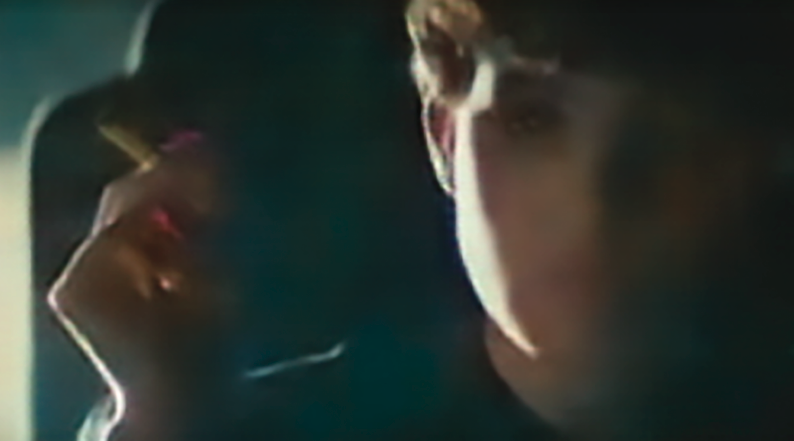
\includegraphics[width=1\textwidth]{figures/c1_intro/blade_runner_still.png}
    \caption{Still from \textit{Blade Runner --- Autoencoded}.}
    \label{fig:c1:blade-runner}
\end{figure}

The training data, of course, was not intellectual property that I had permission to use.\footnote{It should also be noted that I was not even the first person to recreate \textit{Blade Runner} with machine learning. Ben Bogart's work \textit{Watching (Blade Runner)} was also created in 2016 \citep{bogart2016watching} (and built upon earlier research \citep{bogart2008memory,bogart2013context}), which I only learnt of its existence many months after completing my own recreation of the film.}
Ironically, this project and the resulting (and later rescinded) DMCA copyright takedown notice given to the videos on the web platform Vimeo was what catapulted the work to international recognition after an account of these travails was detailed in the news website Vox \citep{romano2016bladerunner}.

\begin{figure}[!htb]
    \centering
    \captionsetup{justification=centering}
    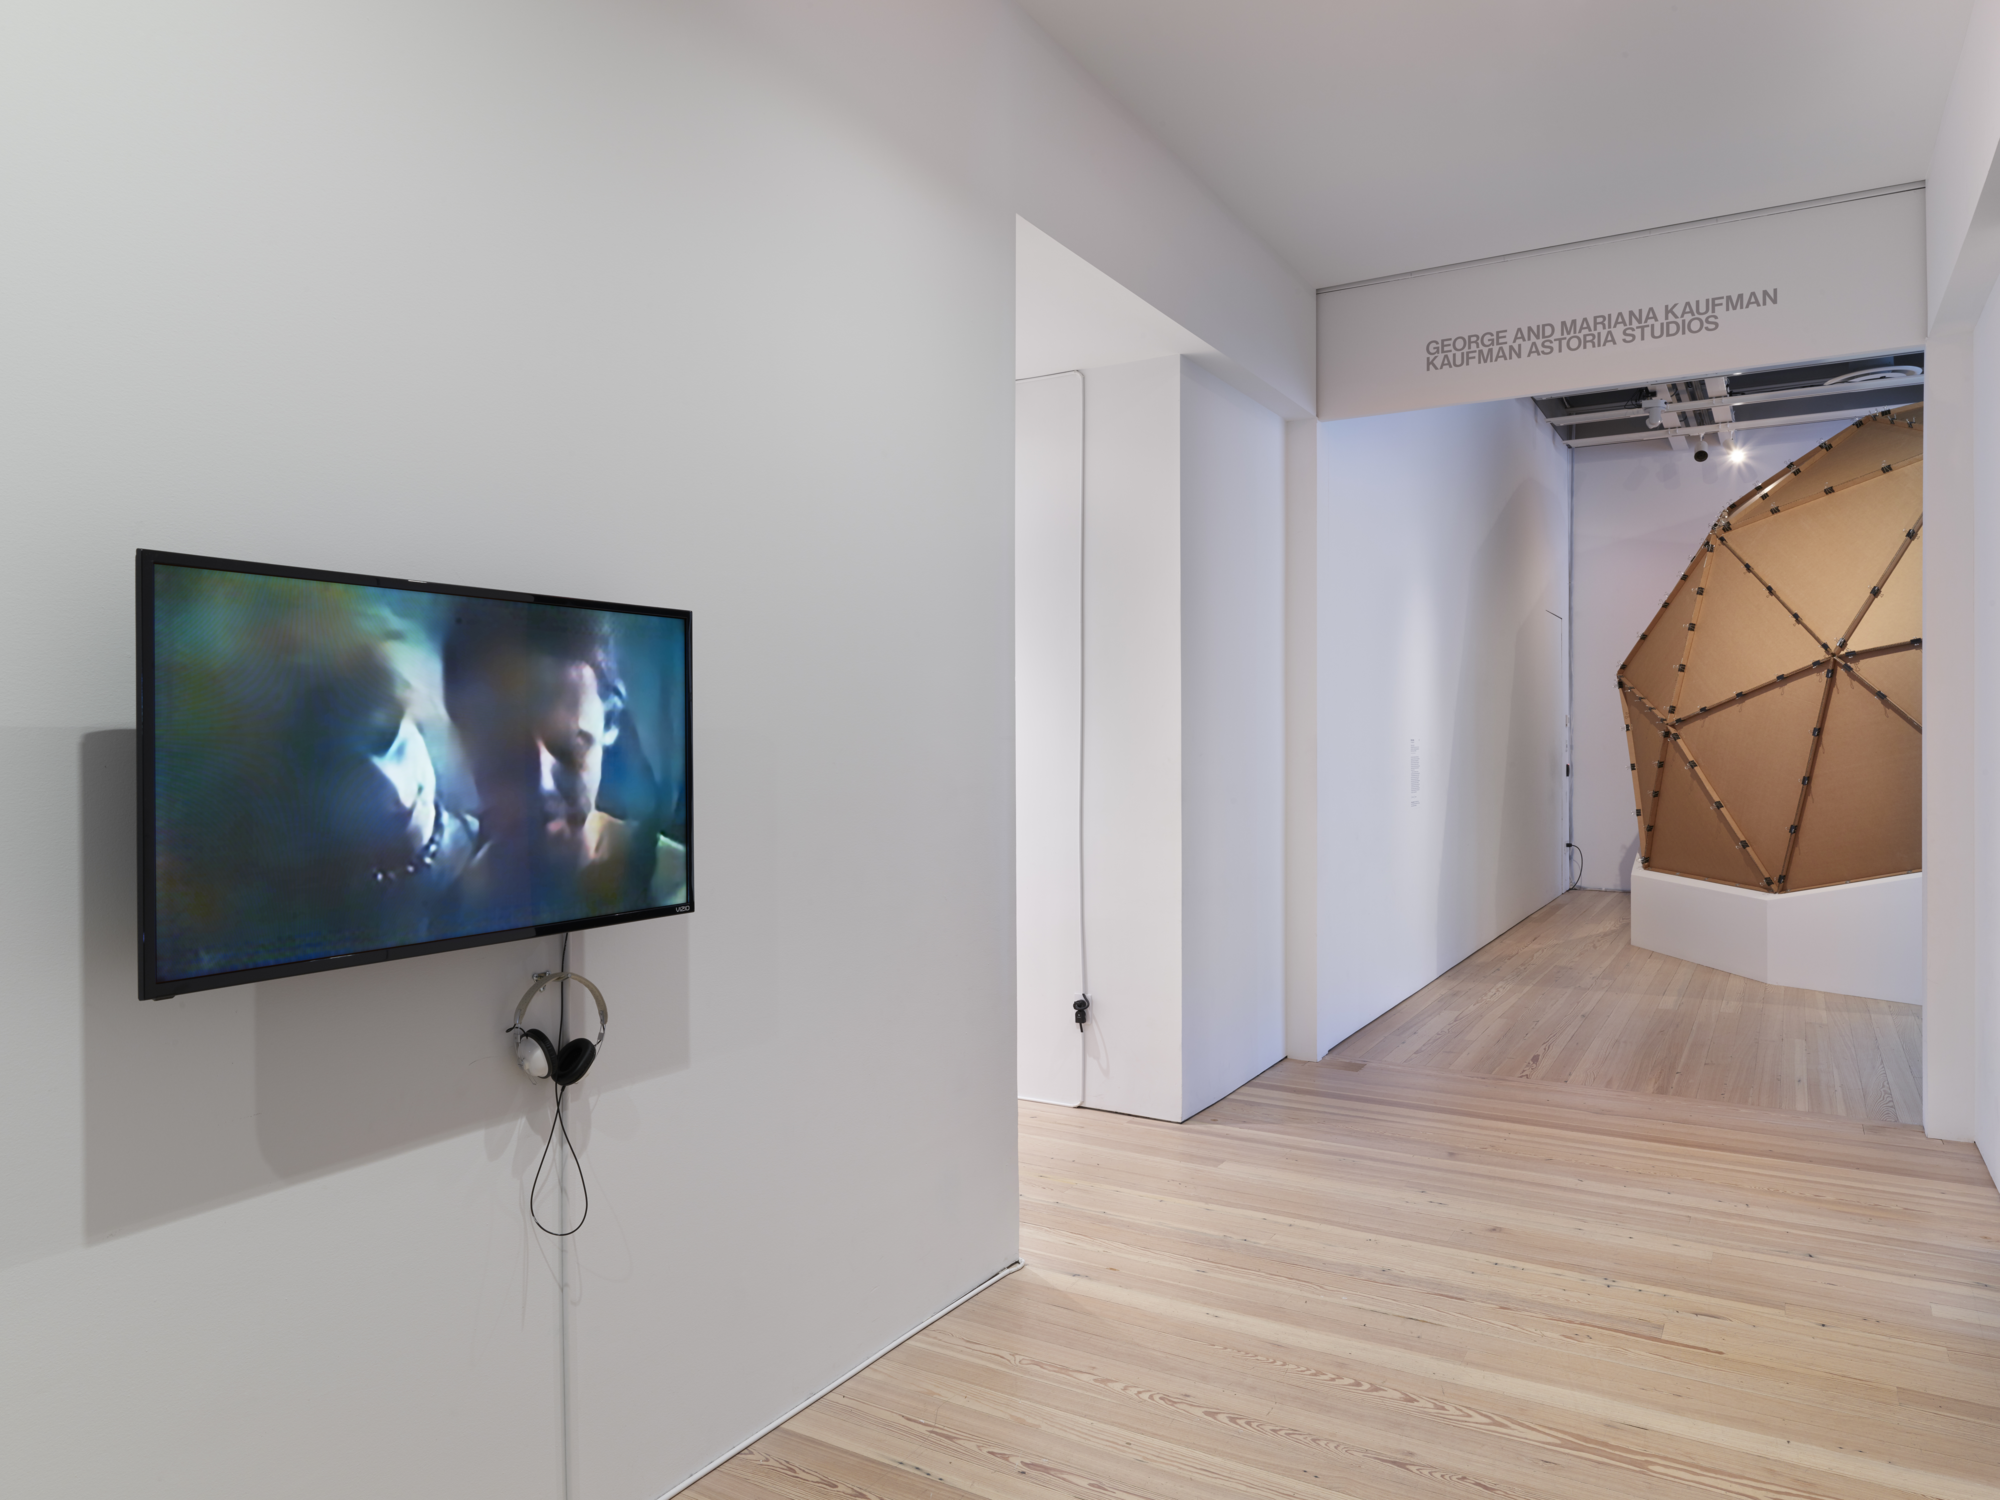
\includegraphics[width=1\textwidth]{figures/c1_intro/whitney-installation-shot.png}
    \caption[Installation view of \textit{Blade Runner --- Autoencoded} at the Whitney Museum of American Art]{Installation view of \textit{Dreamlands: Immersive Cinema and Art, 1905-2016} (Whitney Museum of American Art, New York, October 28, 2016-February 5, 2017). Left to right: Terence Broad, \textit{Blade Runner - Autoencoded}, 2016; Liam Gillick, \textit{Annlee You Proposes}, 2001. Photograph by Ron Amstutz. Image courtesy of the Whitney Museum of American Art.}
    \label{fig:c1:blade-runner-whitney}
\end{figure}

Though I did not face any further legal action from Warner Brothers for  disseminating the work, it was a major cause of personal stress, as I was very often anticipating some form of legal intervention (e.g. a cease and desist notice) from Warner Brothers prior to any exhibition where the work was going to be shown.
An opinion published in the Columbia Journal of Law and the Arts predicted that the work would probably be dealt with as copyright infringement were it tested in an American court \citep{sobel2017artificial}.\footnote{An alternative legal opinion was given by legal scholar Andres Guadamuz, who believed that this would be protected by fair-use or fair-dealing if it were to be tested in court on the basis of parody or pastiche \citep{guadamuz2024personal}.} 
I produced the work before the widespread emergence of NFTs and before there was a large market for AI-generated artworks. 
The money I made from exhibition fees and selling editions of the video work would have been relatively insignificant for a multinational media company. 
Nonetheless, this experience was instrumental in informing the subsequent research presented in this thesis. 
Finding ways of using generative AI that does not rely on data and the intellectual property of others was a key aim for the research presented in this thesis.


\section{Motivation}

My goal was to find ways of training or configuring generative AI models which did not rely on the creation of datasets to produce creative outcomes. 
From working in the AI industry, I had experienced how labour-intensive and time-consuming creating high-quality datasets could be, and it was clear this was a hugely time-consuming aspect of Generative AI research processes.
The second was to find ways of achieving novel outcomes that did not rely on access to high-end resources, for example, those available to large technology companies, including Google DeepMind, NVIDIA, or artists such as Refik Anadol (who reportedly have access to considerable computational resources  \citep{caulfield2022refik}). 
To this end, this research has focussed on exploring methods for training, configuring and customising very high-fidelity models that, when trained conventionally, require supercomputer-level resources. 
As such, this thesis presents a number of useful methods for manipulating, training and controlling these same models in much shorter time periods on consumer-level hardware.

Instead of relying on laboriously or ethically questionable datasets to try and achieve creative outcomes, the work in this thesis details data-free methods that push the possibility space of what can be generated with contemporary neural networks.
The approaches detailed are an attempt to use the intrinsic affordances of these neural networks to create original outputs that would not have been possible using any other technique or technology. 
The work detailed in this thesis is experimental image-making in its truest sense, and I have taken more inspiration from experimental photographers and filmmakers of the 20th Century (such as Harold Edgerton, Hiroshi Sugimoto, and Oskar Fischinger) than from academic researchers.

The driving force that led to each technical breakthrough in this thesis has been technical curiosity. 
When considering a new possible configuration for training an AI or some other kind of intervention, if I couldn’t imagine what the result of that experiment would look like, I would have to build it to find out, regardless of how many weeks or months of work it would take to get there. 
The results presented here are the experiments that produced the most surprising and striking results - sometimes beautiful and sometimes horrifying. 
There were a lot of failed experiments along the way that produced boring, predictable and uninspiring results. 
I’ve spared the reader details of most of these, apart from the few that led to key insights.

\section{Research Methods}

The research breakthroughs presented in this thesis have all come from a technological exploration of what is possible with these new technologies. Much of this research has been conducted in the vein of hacking, in its original meaning from the hacker culture at MIT (Massachusetts Institute of Technology) in the 60s and 70s, where hacking meant `exploring the limits of what is possible, in a spirit of playful cleverness' \citep{stallman2002hacking}. 
This hacking ethos is not an approach that many people were taking in machine learning research when I started this PhD. 
The field was, and still is, very much dominated by orthodoxies and ideology, where theoretical mathematical underpinnings, achieving state-of-the-art performance on some widely used benchmark, and generalisation are most valued by the research communities \citep{birhane2022values}.

\textit{Hacking} was the primary means by which the algorithms in this thesis were discovered, but artistic exploration has also been central to the experimental work described in this thesis. 
When I started this PhD, my plan was to conduct primarily technical research and continue with an artistic practice on the side, maybe using some of the techniques developed in my research. 
Instead, it was an artistic enquiry that led me to the technical breakthroughs in the PhD, not the other way around. 

In his paper \textit{`Art in the sciences of the artificial'}, Stanley argues that in the fields of AI research and artificial life, subjective evaluation is a key driving force of progress for many researchers and practitioners in the field. 
There is a tendency in these research fields to discourage the dissemination of these observations in academic writing and in wider public discourse, something that Stanley worries might `cut off some future discoverers from what could have been their inspirations' \citep{stanley2018art}. 
In this thesis, I have sought to share my subjective position at various times in the thesis, and how that informed the direction of the following research experiments (\S \ref{c8:sec:aesthetic} for a further reflection on this).

Being both guided by, and disseminating this kind of subjectivity is commonplace in research practices in many areas of the humanities, including research methods such as autoethnography \citep{reed1997auto}, or practice-based and practice-led research \citep{candy2006practice}. 

The goal of this research has been at its core, to advance the creative possibilities of these technologies. 
As a practising and internationally recognised visual artist, my subjective understanding of the visual potential and aesthetics of these systems has been one of the central guiding instruments in this research. 
To give any other account of how this research was conducted would be a failure of academic integrity. 

The work  I have done that is described in this dissertation and the contributions made in this thesis were the outcomes of practice-led research. 
The artistic outcomes are not presented as contributions to be assessed as outcomes of the thesis as such, but the process and practice that went into making them are described in an honest account in this thesis. 
Descriptions of artworks that have been made by myself and others using the techniques that have been described in this thesis are detailed in Chapter \ref{ch:impact}.

\section{Overview and Contributions of the Thesis}

The thesis is entitled \textit{Expanding the Generative Space}. 
The throughline of all of the research presented here has been to find ways of going beyond the imitation of training data as the sole method for training generative neural networks. 
Instead, I have been trying to expand the possibility space that generative AI can produce, and the methods described in this thesis are but a few of the ways that this is possible. 

\subsection{Background}

Chapter \ref{ch:background} provides a thorough review of relevant background literature and related research conducted prior to the work presented in this thesis.
This review encapsulated both the technical aspects of machine learning relevant to this thesis, and also its application in creative contexts, whilst also drawing on the broader history of AI methods such as evolutionary algorithms, and their applications for generative processes. 
This chapter also describes notable prior work in relation to attempts to achieve novel outcomes with generative neural networks.

\subsection{Training without Data}

Chapter \ref{ch:unstable_eq} documents the first peer-reviewed and published approach to training generative neural networks without data, one of the three categorical contributions to active divergence methods (\S \ref{survey:nodata}) presented in this thesis.
This work was first published in the paper \textit{`Searching for an (un)stable equilibrium'}: experiments in training generative models without data' at the NeurIPS 2019 Workshop on Machine Learning for Creativity and Design \citep{broad2019searching}.

\subsection{Divergent Fine-Tuning}

Chapter \ref{ch:divergent} documents the first peer-reviewed and published approach to divergent fine-tuning of generative AI models without relying on imitation-based learning.
Divergent fine-tuning is another categorical contribution to active divergence methods (\S \ref{survey:divergent}) presented in this thesis.
This work was first published in the paper \textit{`Amplifying the uncanny'} at the 8th Conference on Computation, Communication, Aesthetics \& X (xCoAx) \citep{broad2020amplifying}.


\subsection{Network Bending}

Chapter \ref{ch:net_bend}, presents the network bending framework and is the third categorical contribution to active divergence methods presented in this thesis (\S \ref{survey:bending}).
This work was first published in the paper \textit{`Network Bending: Expressive manipulation of deep generative models'} at the International Conference on Artificial Intelligence in Music, Sound, Art and Design (EvoMUSART) \citep{broad2020network}, and later extended in the paper \textit{`Network Bending: Expressive Manipulation of Generative Models in Multiple Domains'} for the journal Entropy \citep{broad2021network}.
Network bending has been widely reused and adopted by many other artists and researchers (detailed in \S \ref{c7:sec:net-bend-artworks} \& \S \ref{c7:sec:net-bend-impact}).

\subsection{Active Divergence Taxonomy}

The final contribution of this thesis is the survey and formal taxonomy. 
The large majority of experimental work in this thesis falls under the umbrella term \textit{active divergence}. 
This was first coined by a PhD colleague and friend, Sebastian Berns and his supervisor Simon Colton [\citeyear{berns2020bridging}]. 
The core experimental work in this thesis pre-dates this definition, and I am indebted to Sebastian for summarising the overarching theme of my research, which felt far more disparate when I was working on it until he was able to summarise it in a two-word definition. 
In collaboration with Sebastian and Simon, I expanded on this definition and the paper \textit{`Active Divergence with Generative Deep Learning - A Survey and Taxonomy'} at the International Conference of Computational Creativity in 2021 \citep{broad2021active}.
An updated summary of that survey is presented in Chapter \ref{ch:active_div} and details work completed concurrently by others during the time of this PhD to achieve similar goals.

\subsection{Impact and Discussion}

Chapter \ref{ch:impact} details the impact of the research presented in this thesis and the subsequent work that this thesis went on to inspire. Chapter \ref{ch:discussion} reflects on the work undertaken, how artistic approaches to hacking AI models and training can lead to new forms of understanding, and how AI itself can be used as a material for artistic exploration and expression, a topic that I discussed in the paper \textit{`Using Generative AI as an Artistic Material: A Hacker's Guide'} that I presented at the 2nd international workshop on eXplainable AI for the Arts (XAIxArts) at the ACM Creativity and Cognition Conference \citep{broad2024using}.

\subsection{Conclusion}

Chapter \ref{ch:conclusion} concludes the thesis and reflects further on its contributions.
This chapter also details the limitations of the research presented in this thesis and discusses possible future research directions to take this work further.

\section{Summary}

In the six years that I have been working on this PhD, there has been a huge amount of upheaval in the research field and its impacts on wider society. 
I have seen AI art and generative AI go from a small, quirky community of enthusiasts to a booming industry that has become pitted against the interests and livelihoods of the creative professionals that they are extracting value from.
Hopefully, the approaches to working with AI described in this thesis can help others to find ways of using and working with generative AI which does not rely on the mass stealing and exploitation of creative professionals but instead fosters new ways for creative people to use generative AI in ways that creative people will always do: to deliberately break, misuse and adapt technologies far beyond the intended purpose to forge new forms of creative expression.


\chapter{Background}
\label{ch:background}

\section{Introduction}

This chapter serves as a survey of relevant background literature predominantly available prior to me undertaking my experimental research.
The majority of the chapter outlines the technical basics of machine learning, neural networks and generative modelling.
Further, the chapter also describes relevant research conducted in areas including computation, creativity, generative systems and divergent thinking prior to the advent of deep learning circa 2011-12 \citep{krizhevsky2012imagenet}.

\section{Computation \& Creativity}

Since the advent of automated computing machines, and the idea of writing programs to give these machines instructions to follow, the idea of using computers to develop artefacts deemed creative has been long imagined. 
Ada Lovelace, the woman considered to be the first ever computer programmer, imagined that programmes for Charles Babbage's unfinished Analytical Engine could ‘compose elaborate and scientific pieces of music of any degree of complexity or extent’.
Lovelace however, did not think that computers could originate creativity themselves, declaring ‘The Analytical Engine has no pretensions whatever to originate anything. I can do [only] whatever we know how to order it to perform.' \citep{lovelace1843notes}.

Alan Turing took an opposing viewpoint to Lovelace on this question, stating that this objection would be better posed as ‘a machine can never take us by surprise’, countering that ‘Machines take me by surprise with great frequency [...] because I do not do sufficient calculation to decide what to expect them to do.’ \citep{machinery1950computing}
This reframing from originality to surprise shifts the emphasis from an action by the machine to an evaluation based on a human reaction. 
Turing develops this further, by describing a scenario called \textit{The Imitation Game}, where a computer would be evaluated through a text channel and asked questions by an evaluator who would then attempt to differentiate whether it was human or not. 
If the evaluator considered the computer output to be from a human, this would be a threshold for determining simulated intelligence.
This method for evaluating computational intelligence is commonly referred to as the Turing test. 

In his description of the imitation game, Turing took seriously the idea of a computer being able to develop creative work. 
In the paper \textit{`Computing Machinery and Intelligence'} he muses about a machine writing a sonnet, and then, through the viva voce style of examination, being able to critically defend the work against a human interrogator based on criteria of aesthetic value, originality and of potential subjective readings of proposed changes to the language used in the work \citep{machinery1950computing}.

The idea that the bar for Artificial Intelligence (AI) is to convincingly imitate human behaviours, is one that has long been an anchor for research in the field. 
Imitation is central to much of how we train machine learning, neural networks and generative models, importantly imitation alone is not broadly considered a benchmark for intelligence.
An alternative theoretical test for computational intelligence is the Lovelace test, where a computational program would pass the test a) it can generate an original artefact (poem, musical score, novel, idea) that can be reproduced and b) the creators of the program can not explain how it has found that solution \citep{bringsjord2003creativity}. 

\cite{ward2020computational} argues that Turing's characterisation of Lovelace's lack of faith in the possibility for the analytical engine to produce origination (that he equates with surprise) is a mischaracterisation and misunderstanding of the debates around mechanisation and origination that were happening during the industrial revolution. 
In the same notes where she makes her famous objection, she also goes on to say that the analytical engine has the power to offer new perspectives by combining theories in new ways \citep{lovelace1843notes}.
 Lovelace's remarks demonstrate the creative value of human-machine interaction, where she `understand[s] mechanicity not as inherently creative or uncreative but as a mode through which new kinds of creativity are possible' \citep{ward2020computational}.

\subsection{Theories of Creative Processes}

Creativity itself is broadly agreed as a well-defined concept, though there are some differences in definition. 
Narrower definitions of creativity refer to the cognitive processes involved in culturally understood creative activities, such as 'pieces of music, sculpture, painting, poems or other things that are taken or presented as art' \citep{wiggins2015evolutionary}.
Creativity though, is used much more broadly in common language. 
It can also be applied to acts, ideas or behaviours outside of the realm of art-making, such as scientific fields, sports, economic activities or even mundane, day-to-day activities.


A broader definition of creativity is that it is an act that produces something \textbf{new and original} \citep{kaufman2021overview}. This act needs to be task-appropriate, fulfilling the requirements of whatever the original task set out. 
However, theories of how creativity is achieved, what facilities it, and how it is recognised and evaluated are far more disparate and less agreed upon. 

Theories of what makes a person creative tend to focus on a summation of different elements.
The componential model of creativity proposes that three interconnected variables are key to individual creativity.
First, there are domain-relevant skills and knowledge, such as a technical skill or specific talent.
Secondly, there are skills relevant to creative processes, such as a tolerance for ambiguity and a willingness to take certain risks.
Finally, intrinsic motivation is needed to take part in an activity because it is enjoyable and meaningful \citep{amabile1983social}.

There are many other theories of creativity, pertaining to evaluating individual persons' creativity, creative collaborations, understanding traits of creative peoples and situations that best facilitate creativity and how creativity is evaluated from a historical or cultural perspective. 
The outline in the rest of this section will only cover theories or models of creative processes which have been developed in order to understand how to enhance and replicate creative acts, and in some cases, so that they can be partially or fully automated with computation.

\subsubsection{Convergent and Divergent Thinking}

The psychologist J.P. Guilford set out a series of traits and cognitive processes specific to creative activity. Those are ideation fluency, ideation novelty, synthesising ability and redefining ability, sensitivity to problems and evaluating ability \citep{guilford1950creativity}. 
The fluency with ideas generated, the novelty of said ideas and the ability to then critically evaluate those ideas and pick the best one are some of the most important traits for creative people.\footnote{Notably, Guildford motivates this early research into the psychology of creativity because of the rise of \textit{thinking machines} (aka digital computers). Imagining their eventual knock-on effect on the labour market and a future industrial revolution of intelligence being automated, Guildford muses that the only economic value left of human brains would be in the creative thinking they are capable of \citep{guilford1950creativity}. A viewpoint I am not unsympathetic to.}

Guilford later builds on this theory, expanding the thinking processes needed in creative thinking, in particular the processes that are required for the production of creative ideas.
He differentiates two kinds of productive thinking that are required for creativity; divergent and convergent thinking. 
Convergent thinking is the focusing of ideas down to a single correct answer. 
Divergent thinking is the diametric opposite, which is the ability to generate new and different ideas. 
In the context of modelling creative acts, these two types of thinking are also called idea generation and idea evaluation \citep{guilford1957creative}.

Of these two modes of productive thinking, Guilford believes divergent thinking is that which is more representative of and unique to the creative process. 
He considers factors of fluency, flexibility and original thinking as products of abilities in divergent thinking.
Guilford's ideas about divergent thinking went on to inspire many other aspects of research, such as the Torrance test for creative thinking \citep{torrance1966torrance}.

\subsubsection{Associative Creativity}

Associative creativity is the theory that creative people or creative acts are made when connections are made between remote concepts or ideas \citep{mednick1962associative}. 
Koestler coined the term \textit{bisociation} to describe a cognitive process where two or more concepts are combined to create a new concept \citep{koestler1964act}.
This model of creativity is also referred to as \textit{combinatorial creativity} \citep{boden2004creative}.

\subsubsection{Evolutionary Theory of Creativity}

Evolutionary theory states that the genetic structure of living beings is constantly changing through processes of random mutation and selection. Selection is carried out in two ways: \textbf{natural selection} is the process of fitness through living beings surviving long enough to reproduce sexually and transmit their genome. \textbf{Sexual selection} is the process by which organisms make preferential choices regarding which partners to mate with based on particular attributes.

An evolutionary approach to how ideas are generated and selected in creative acts was proposed by \cite{campbell1960blind}, where he stated that the process of blind variation and selective retention in thought achieves innovation (aka creativity).
According to Campell, this occurs through the internal emitting of thoughts, a process which lacks prescience and foresight.
Campbell justifies this as a blind process, stating that `once the process has blindly stumbled into a thought trail that ``fits'' the section criterion, accompanied by the ``something clicked'' or ``Eureka'' that usually marks the successful termination of the process' \citep{campbell1960blind}.

\subsection{Computational Creativity}

Computational creativity is a subfield of AI research which investigates developing software that exhibits creative behaviours which unbiased observers would perceive as being creative \citep{colton2012computational}.
Computational creativity research is usually preoccupied with artefact generation in domains that are culturally recognised as being creative, such as poetry, story generation, images or music.
The mechanics of the system and how they are constructed to imitate the creative faculties of humans is the central area of exploration, whereas the quality of the generative process and the outputs from them is usually a secondary concern.

Computational creativity differentiates itself from the practice of building and evaluating creativity support tools, such as those commonly researched in the field of HCI (Human-Computer Interaction) (\S \ref{c2:subsec:cst}).
Famously, the tagline at the 3rd International Conference on Computational Creativity in 2012 was ‘scoffing at mere generation for more than a decade’, though this has become an increasingly divisive phrase within the computational creativity community \citep{ventura2016mere}.

\subsubsection{Human-AI Co-Creation}
\label{c2:subsubsec:co-creativity}

Human-AI co-creation (also referred to as co-creativity) is a subfield of computational creativity research where the creative responsibility is shared between the software and the human interacting with it \citep{candy2002modeling}.
This framing positions the software as a creative collaborator, as opposed to an independent creative agent or tool only for supporting human creativity \citep{feldman2017co}.

\subsection{Metacreation}

Metacreation is the practice of developing software that demonstrates creative behaviour \citep{whitelaw2004metacreation}. 
In metacreation practice, the objective is not just to develop software, but to produce and present artistic works derived from the software, to validate their success. 

\cite{eigenfeldt2012evaluating} describe five viewpoints that should be considered when evaluating a metacreation system: (1) the designer of the system, (2) the audience for the derived artworks, (3) academic experts, (4) domain experts, (5) results from controlled experiments.
This emphasis on audience evaluation and domain expertise differentiates metacreation research from computational creativity, where the emphasis is in the inherent soundness of the processes encoded in the system architecture \citep{colton2008creativity}.

\subsection{Creative Computing}

Creative computing is an academic discipline\footnote{Creative computing is the academic discipline I am most at home with, having done my BSc and (integrated) Msci in Creative Computing at Goldsmiths, University of London, and more recently, being employed as a Senior Lecturer at the Creative Computing Insititute at University of the Arts London.}
that builds from the alternative computing scenes of the latter half of the 20th Century, which include \textit{hacking} and \textit{the demoscene}. 
Hacking and the creation of a \textit{hack}, is a specific sense of creative invention with given materials in the context of electrical engineering and the academic environments researching this in the 1960s in MIT and Stanford \citep{wark2006hackers}. 
Though not exclusively used to describe computer code or a technical system, a hack had to `be imbued with innovation, style and technical virtuosity' \citep{levy1984hackers}.

Hacking later became associated with the breaking of digital security and performing acts of digital trespassing and accessing confidential information, a practice that has retrospectively been called cracking. 
Cracking copy protection on home computer systems, for the distribution of games led to the evolution of the demoscene. 
 In the demoscene, visual and audio programs were written and freely shared, where value was determined, for example, as follows: ‘more graphical elements, more mathematical effects and more sounds made a better demo, while bugs, glitches, and irregularities made the demo worse’ \citep{carlsson2019forgotten}.

Creative computing refers to the practice of using computing technologies to create expressive artefacts rather than something that is strictly functional \citep{yang2016promoting}.
In creative computing, programming is the main tool that the creator uses to generate an artefact, and coding is the medium used to express human creativity. 

Creative coding is often carried out with creative coding frameworks, which are libraries, programming languages, or visual programming interfaces (such as node-based programming). 
Creative coding frameworks tend to focus on supporting visual rendering, audio processing and supporting human interaction with these frameworks. 


\subsection{Creativity Support Tools}
\label{c2:subsec:cst}

Creativity support tool (CST) is the term given to software programs that are designed to facilitate creative acts or enhance a user's creativity \citep{shneiderman2002creativity}. 
For CSTs, the graphical user interface (GUI) is of high importance \citep{shneiderman1999user}. 
CSTs can be used to facilitate many varieties of tasks such as searching, visualising, consulting, thinking, exploring, composing, reviewing and disseminating \citep{shneiderman2002cst_tutorial}.

With creativity support tools, the code is neither seen as acting in a creative way in its own right nor is it a medium for humans to be creative. 
Creativity support tools are independent pieces of software that can facilitate creativity but are not seen as being responsible for contributing to the creative process in their own right, as is the case with human-AI co-creativity (\S \ref{c2:subsubsec:co-creativity})

\subsection{Computational Models of Creative Processes}

There is a large existing literature on computational models that encode specific theories of creative processes, or specific attributes that are deemed essential for creative people to have.
This subsection covers a non-exhaustive selection of these methods described in the literature.

\subsubsection{Evolutionary Computation}

Evolutionary computation refers to algorithms that are inspired by the process of biological evolution to perform some form of optimisation. 
The most commonly used evolutionary algorithm is the \textit{genetic algorithm}, which is inspired by many of the processes present in biological evolution, such as random mutation, sexual selection, or (chromosomal) crossover.

Genetic algorithms require some kind of \textit{fitness function}, that determines the quality or performance of an individual solution to whatever optimisation problem is trying to be solved. 
This is analogous, and in some ways similar to the \textit{loss functions} used in machine learning algorithms (\S \ref{c2:sec:ml}). 

A genetic algorithm requires a genetic representation of the solution domain. 
This representation is usually a linear vector, and is often binary, with a fixed length representation, which allows for easy implementation of genetic operations such as crossover. 
The parameters in the genetic representation need to be carefully selected as they determine the \textit{solution space}.
Genetic algorithms are a stochastic optimisation process for exploring a \textit{fitness landscape} and converging onto a high-quality solution \citep{back1996evolutionary}.

\subsubsection{Novelty Search}

Novelty search is an algorithm developed by \cite{lehman2008exploiting}, first used to guide evolutionary algorithms, where there is no set objective or fitness function.
Instead, the search for novelty in the behavioural space of an evolutionary agent is the sole criterion. \cite{lehman2010efficiently, lehman2011abandoning,lehman2011novelty} argue that by abandoning prescriptively defined objectives, novelty search algorithms can better search the possibility space of an evolutionary landscape, and they show that this approach can lead to both unexpected and more optimal behaviours in evolutionary agents.
This approach to open-ended learning in evolutionary algorithms has inspired more recent developments in the space of open-ended reinforcement learning \citep{wang2020enhanced} (\S \ref{c2:subsec:reinforcement} for a definition of reinforcement learning).

\subsubsection{Bayesian Surprise}

Bayesian Surprise \citep{itti2005bayesian,itti2009bayesian} is an algorithm that takes inspiration from information theory and Bayesian statistics, that gives a mathematical formulation for surprise. 
This computational measure closely correlates with human attention, through the measurement of gaze shift of human participants watching television broadcasts.

\subsubsection{Intrinsic Motivation}

In agent-based AI modelling, intrinsic motivation is defined as goals or objectives for the agent that are not determined by external stimuli or reward functions (aka external motivation), but by the internal state of the agent itself. 
Intrinsic motivation can be applied in reinforcement learning agents \citep{chentanez2004intrinsically} (\S \ref{c2:subsec:reinforcement}), and is motivated by the proposition that not all objectives are universally useful \citep{barto2013intrinsic}.
Intrinsic motivation in AI is grounded in evolutionary theory \citep{singh2010intrinsically}, where an otherwise single mathematical function that defines a universal fitness function does not account for all behaviours and evolutionary strategies exhibited in real-world biological evolution.

\subsubsection{Compression Progress}

Compression progress \citep{schmidhuber2008driven} is a theoretical approach to training agents that relates to novelty search \citep{lehman2008exploiting} and intrinsic motivation in RL agents \citep{chentanez2004intrinsically}.
Schmidhuber defines compression progress as an agent that is constantly trying to efficiently represent prior actions in an environment, whilst constantly seeking out new experiences that would satisfy an `intrinsic curiosity reward', which would drive the agent toward seeking out novel and unpredictable experiences.
Schmidhuber argues that this framework could be used for mathematical discovery, as well as art-making through `subjective beauty'.

\subsubsection{Combinatorial Creativity}

Combinatorial creativity is the description of a creative process where two or more concepts are combined together to make new ones \citep{boden2004creative}. 
This concept is essentially a rehashing of the concept of bisociation first proposed by \cite{koestler1964act}. 
Combinatorial creativity has been explored extensively in the context of computational creativity research \citep{zarraonandia2017using, guzdial2018combinets, guzdial2018combinatorial} and in explaining the psychology of scientific discovery \citep{simonton2021scientific, simonton2022serendipity}.

\subsection{Enacting Creative Processes in the Computational Arts}

Many artists have explored models of creativity and creative processes through practice-based enquiry.
Artists have made substantial contributions to this field and our understanding of non-human creativity, and the interactions between people and computers in exploring new possibilities for creative autonomy and creative collaboration.
A selection of these efforts is detailed in the following.

\subsubsection{Human-AI Co-Creation}

Harold Cohen, the pioneering computational artist, developed and worked with the AARON program and robotic painter (using an XY plotter), to co-create paintings between 1972-2010 \citep{cohen2016harold}. 
The program underlying AARON was developed by Cohen himself \citep{cohen1995further}, using deterministic software that was in a constant process of development. 
AARON has been described as a form of meta-art (or metacreation) \citep{mccorduck1991aaron}, where the artwork itself is the creation of a process that creates art.

The artist Sougwen Chung extends Cohen's work to create a practice that is centred around performative works where Sougwen collaboratively and interactively \citep{benediktsson2019human}.
Sougwen uses this practice to explore themes of increasing automation and co-existence between humans, algorithms and machines \citep{voss2021conversation}.

\subsubsection{Evolutionary Arts}

Many artists have explored the biological theory of evolution and evolutionary computation for artistic experimentation.
Karl Sims seminal experiments explored evolutionary computation for the creation of computer graphics \citep{sims1991artificial} and 3D morphology and behaviours in artificial creatures \citep{sims1994evolving, sims2023evolving}.

The artist William Latham, alongside collaborator Stephen Todd, developed the FormGrow to evolve 3D computer models resembling organic life \citep{latham1992evolutionary}, with the aesthetic preference of the artist guiding the evolutionary process \citep{lambert2013emergence}.
Using aesthetic preference to guide evolutionary systems was also utilised in the work \textit{Cellular Forms}, where \cite{lomas2014cellular} built his own user interface to interactively explore the possibility space of simulations of growing cellular organisms.

\section{Machine Learning}
\label{c2:sec:ml}
Machine learning algorithms are algorithms that automatically improve from training data or experience. 
Given training data, a machine learning algorithm will build a model to make predictions or decisions without explicitly being told what decisions to make. 
Most machine learning algorithms use some form of optimisation and are optimised to minimise a loss function that is generally predetermined and task-specific. 
The process of optimising a machine learning model is referred to as \emph{training}. 
When training a machine learning model, the loss function on the training data will be minimised with the goal of maximising the accuracy for the specific task. 
The model is generally evaluated on a separate test dataset that contains data not used during the training phase \citep{murphy2012machine}.

\subsection{Supervised Learning}

Supervised learning algorithms build models based on training data that contain the desired set of output and inputs. 
This type of training data is referred to as \emph{labelled data}. 
A labelled dataset will consist of pairs of data, where every input will be given with a corresponding output. 
Labelled datasets are in most cases hand-labelled by human users who ideally have expertise in the subject domain.
Three of the most common tasks in supervised learning are \emph{classification}, \emph{regression} and \emph{metric learning}. 


\subsubsection{Classification}

In classification, each data sample $x$ will be paired with a vector $c$ that represents the class label. 
The machine learning model will take $x$ as an input and output a prediction $c'$. 
The objective during training is to maximise that the probability of the prediction $c'$ will match the value of the true label $c$ \citep{murphy2012machine}. 

\subsubsection{Regression}

In regression, each data sample $x$ will be accompanied by an output $u$, where the output values are numerical values within a given range. 
The model will learn to output predictions $p'$ for input $x$. The goal of training a regression model is to learn a model that can generalise to unseen data, where the input and output values are not necessarily present in the training data but can be inferred based on the examples given in the training data \citep{murphy2012machine}. 

\subsubsection{Metric Learning}
\label{c2:subsubsec:metric}

The goal of metric learning is to learn a distance function between given samples, that can be used to estimate how similar or dissimilar samples are. 
The model learns to provide a distance function $d(x,y)$ for input examples $x$ and $y$. In the labelled dataset, input examples are usually accompanied by a vector label $c$ donating the identity of the input example. 
When training a model, the goal is usually to minimise the distance between samples that have the same identity but maximise the distance between samples that have separate identities \citep{kulis2013metric}.

\subsection{Unsupervised Learning}

Unsupervised learning algorithms find patterns in data where there are no given labels. 
Unsupervised learning methods find patterns and structures within data without guidance, either by learning discriminative features or capturing patterns as probability densities. 
The two most common tasks in unsupervised learning are \textit{clustering}, \textit{dimensionality reduction} and \textit{generative modelling}.

\subsubsection{Clustering}

Clustering is the task of grouping data into clusters such that data grouped together in the same cluster are more similar to each other than data in another cluster. 
Examples of algorithms used for clustering are K-means, Gaussian mixture models or density-based clustering methods \citep{xu2005survey}.

\subsubsection{Dimensionality Reduction}

Dimensionality reduction is the task of transforming high-dimensional data into a lower-dimensional representation that still retains key characteristics present in the original data. 
Examples of algorithms used for dimensionality reduction are Principle Components Analysis (PCA) \citep{pearson1901liii}, t-Distributed Stochastic Neighbour Embedding (t-SNE) \citep{hinton2002stochastic} and autoencoders (\S2.2.1). 

\subsubsection{Generative Modelling}

Generative modelling is the task of learning a function that can generate a given data distribution. 
A generative model will give a joint probability distribution between the observable and target variables. 
Approaches to generative modelling include Gaussian mixture models, hidden Markov models and neural networks. 
An overview of generative model approaches using deep neural networks is given in Section \ref{c2:sec:gen-nn}.

\subsection{Reinforcement Learning}
\label{c2:subsec:reinforcement}

Reinforcement learning (RL) is a form of agent-based modelling, where the agent learns how to behave in an environment by performing actions and receiving feedback in the form of penalties or rewards \citep{sutton1999reinforcement}. 
The most commonly used algorithm in RL is Q-learning, where the agent learns the value of taking a specific action in a specific state in the environment \citep{watkins1992q}.
Over the course of learning, a Q-table matrix records values for each state-action pair and gradually improves the policy.

\section{Artificial Neural Networks}

Artificial neural networks are ensembles of connected units that are meant to loosely model the synaptic structure of biological neural networks. 
The first artificial neural network was the Mark 1 Perceptron \citep{rosenblatt1958perceptron}, initially a physical circuit that was designed to perform the binary classification of images captured from a sensor array. 
The values of the weights between connections were encoded using potentiometers with a learning rule updated with electric motors. 
Later the perceptron architecture was modelled in software rather than hardware, with weight parameters and values encoded as real-valued numbers. 
The term perceptron was later used to denote a unit (or node) within a larger network and is used to this day in larger network architectures such as Muti-Layered Perceptrons (MLP).

The term MLP usually denotes a fully connected feed-forward neural network architecture with one or more hidden layers \citep{rosenblatt1958perceptron}. 
However, MLP can also be used to refer to neural networks with more complex topological arrangements between nodes. 
MLPs can employ different non-linear activation functions, such as $\tanh$ \citep{kalman1992tanh} and the sigmoid function ($\sigma$) \citep{han1995influence}.
A significant advance in training MLP networks came with the backpropagation algorithm \citep{werbos1974beyond}, where the gradient of the loss function is calculated and backpropagated through the network graph and used to adjust the weight parameters of the networks with respect to a single input pass of the network. 
This learning algorithm is referred to as textit{gradient descent} when the learning rule is applied after performing a forward pass on every datum in the dataset, and \textit{Stochastic Gradient Descent} (SGD) when it is applied after every sample or every batch of samples. 

\subsection{Deep Learning}

Deep learning is a term used to describe artificial neural networks with many hierarchical layers that produce \textit{deep} network structures. 
Earlier attempts to make neural network architectures with many layers were hampered by computational resources and limited availability and storage of data. 
The first major breakthrough in the efficacy of training deep generative models was to train a hierarchy of restricted Boltzmann machines \citep{ackley1985learning} as pretraining for a deep autoencoder network \citep{hinton2006reducing}. 
The first major breakthrough in efficacy and efficiency of training deep neural networks on Graphics Processing Units (GPU) was with AlexNet \citep{krizhevsky2012imagenet} which won the 2011 ImageNet Large-Scale Vision Recognition Challenge (LSVRC) for image classification \citep{russakovsky2015imagenet}. 
Additional breakthroughs in novel activation functions such as the Rectified Linear Unit (RELU) \citep{nair2010rectified}, and optimisation algorithms with improved performance and stability over SGD, such as \textit{RMSProp} \citep{tieleman2012lecture} and \textit{Adam} \citep{kingma2015adam} were key to improving the reliability of fundamental training methods for large scale deep neural networks.


\subsection{Neural Network Architectures}

Traditionally the most commonly used architecture for neural networks was the fully connected MLP, where every node in the layer of the network (perceptron) is connected to every other node in the previous and following layers. 
In more complex architectures, techniques like \textit{skip connections} \citep{raiko2012deep,graves2013generating,hermans2013training} are used to connect nodes from layers that have intermediate layers in between them. 

There is a range of other neural network architectures that have been found to have good performance for specific domains. 
What follows is a discussion of some of the most common.

\subsubsection{Convolutional Neural Networks}

A convolutional neural network (CNN) \citep{fukushima1982neocognitron} is a network that uses a structure of shared weights based on convolutional kernel filter functions, where the parameters of the convolutional kernel are learned. 
The kernel functions are repeated across the breadth of the input (in a sliding window fashion where the gap between each instance of the filter being applied is known as the \textit{stride}), ensuring that the learned features are equivariant to translation. 
CNN architectures are most commonly used in a 2-dimensional (2D) form for image processing, but 1D and 3D convolutional architectures are sometimes used for processing audio and 3D voxel data. 
In the architectures of generative models, transposed convolutions are commonly used to iteratively upsample learned features into a high-dimensional output.

\subsubsection{Recurrent Neural Networks}
\label{c2:subsubsec:rnn}

Recurrent neural networks (RNN) are neural network architectures that have connections between nodes along a temporal sequence. 
Connections from a previous temporal state into an existing state allow RNNs to exhibit dynamic temporal behaviour. RNNs are trained on sequential data, with activations from the previous state of the network feeding into the current state, and are able to process temporal data of variable lengths. 
Traditional RNNs suffer from the exploding and vanishing gradient problem, where the error signal backpropagated through the temporal state of the network has a tendency to vanish completely and prevent the network from learning or to explode and catastrophically lose information that had been acquired in training \citep{hochreiter1998vanishing}. 
RNN architectures such as the Long-Short Term Memory network (LSTM) \citep{hochreiter1997long} or the Gated Recurrent Unit (GRU) \citep{cho2014properties} are specifically designed to avoid this problem by using gates that can retain information within the network for long periods of time and allow the network mix information from high frequency and low-frequency components. 

First introduced in the context of machine translation, the attention mechanism was introduced to improve the ability of RNNs to attend to different parts of the input and output sequences when predicting the next token \citep{bahdanau2014neural}. 
This attention mechanism has become widely used in many other domains and is now central to the functioning of large language models using the transformer architecture (\S \ref{c2:subsubsec:autoregressive}).

 
\section{Generative Neural Networks}
\label{c2:sec:gen-nn}

Generative models are neural networks that learn a set of neural network parameters that approximately model a target data distribution. 
This was generally seen as a difficult problem, especially for images and audio, until advances were made in core techniques (listed below) and architectures were combined. 
Since 2015 there has been a lot of interest in generative models from varying research areas (computer graphics, audio Digital-Signal Processing (DSP), Human-Computer Interaction (HCI)) and creative communities, artists, musicians etc, because of their ability to produce artefacts of high cultural value. 

When training a generative model, a network architecture will be defined and the parameters of the network will be randomly initialised.
The network will generate a sample $p'$ given an input vector $x$. 
Over the course of training using some learning rule, generated samples are optimised to resemble samples drawn from the target distribution $P$, eventually leading to a set of parameters that produces the approximate distribution $P'$.

All deep generative models, and in particular, ones that generate high dimensional data domains like images, audio and natural language, will have some level of divergence $D(P||P') \geq 0$ between the target distribution $P$ and the approximate distribution $P'$, because of the complexity and stochasticity inherent in high dimensional data. 
The goal of all generative models is to minimise that level of divergence, by maximising the likelihood of generating the given data domain.

\subsection{Approaches to Modelling Data}

Approaches to modelling data distributions can be separated into three categories: explicitly - where modelling the likelihood of the data distribution is learned explicitly in the objective function, such as with autoencoders, autoregressive models; approximately - where an approximation of the target distribution is learned, as is the case with variational autoencoders and reverse diffusion models; or implicitly - where the target data distribution is not modelled directly but is learned implicitly through an indirect training process as is the case with generative adversarial networks.
In the following subsection, more detail of the varying approaches to modelling data distributions is given. 

\subsubsection{Autoencoders}

An autoencoder is a symmetrical neural network that learns to reduce the dimensionality of a data domain.
The first part of the network, the \textit{encoder}, takes data $x$ from the input domain and compresses it into a latent representation $z \in Z \in \mathbb{R}$. 
The other half of the network is the \textit{decoder}, which takes the latent encoding that reconstructs the input \citep{kramer1991nonlinear}. 
An autoencoder is trained to minimise a reconstruction loss which is usually the mean-squared error.
The encoder can be thought of as a learned algorithm for dimensionality reduction, and the decoder as the inverse function. 
Autoencoders are used for the tasks of dimensionality reduction, representation learning and generative modelling.

The Variational AutoEncoder (VAE) \citep{kingma2013auto, rezende2014stochastic} advances the traditional autoencoder.
It forces a distribution on the latent variable and uses Kullback-Liebler divergence (KLD) in the loss term to penalise the encoder if the posterior distribution $q_{\phi}(z|x)$ deviates too far from the prior distribution $p_{\theta}(z)$. 
Noise is injected into the latent space of the VAE during training.
This means a VAE models a data distribution approximately, in contrast with a traditional autoencoder which models a distribution explicitly and can only therefore model the lower bound of the log-likelihood of the data. 
Equation \ref{eq:vae} shows the two terms that make up the VAE loss, the KLD and reconstruction losses:

\begin{equation}
\label{eq:vae}
L(x) = -D_{KL}(q_{\phi}(z|x)||p_{\theta}(z)) + E_{q_\phi}(z|x)(log_{p_{\theta}}(x|z))
\end{equation}

\subsubsection{Generative Adversarial Networks}

The Generative Adversarial Networks (GAN) training framework \citep{goodfellow2014generative} is a method of training generative models without directly approximating the target data distribution. 
Two networks, the generator $G$ and discriminator $D$ are set against each other in a zero-sum mini-max training regime. 
The discriminator is optimised to correctly classify real samples from a training set and fake samples from the generator, where the generator is optimised to fool the discriminator into predicting its samples are real, using the value function defined in Equation \ref{eq:gan}: 

\begin{equation}
\label{eq:gan}
\min_{G}\max_{D}\mathbb{E}_{x\sim p_{\text{data}}(x)}[\log{D(x)}] + \mathbb{E}_{z\sim p_{\text{z}}(z)}[1 - \log{D(G(z))}]
\end{equation}

\subsubsection{Auto-Regressive Modelling}
\label{c2:subsubsec:autoregressive}

An autoregressive generative model learns a conditional probability of a single output element based on the preceding elements. 
Like RNNs, autoregressive models can be used to model sequential data of variable length, however, unlike RNNs the internal state of the network from previous time steps is not fed back into the state of the present time step. 
When generating from a trained autoregressive model, generated samples can be fed back into the model to generate novel continuous sequences.

The transformer architecture used foremostly in large language models (LLMs) \citep{vaswani2017attention}, makes use of the attention mechanism first introduced in RNNs \citep{bahdanau2014neural} (\S \ref{c2:subsubsec:rnn}), but removes the recurrent part of the model architecture.
In transformers, a fixed window of tokens (aka context length) is both given as input and output to the model.
In the generative context, the output to the model is offset from the input by a single token, and the model is trained to autoregressively predict the next token in the output based on the input, an approach most famously used in the GPT (Generative Pre-trained Transformer) class of models \citep{radford2018improving, radford2019language,brown2020language}.

Autoregressive modelling has also been applied to image generation.
PixelCNN uses convolutional neural networks to generate images pixel-by-pixel using neighbouring pixels to determine what the next pixel should be \citep{van2016conditional}.
This can be used for both image in-painting, completion and unconditional image generation.
VQ-VAE (Vector-Quantised Variational Autoencoder) adapts the autoencoder approach so that the encoder produces discrete represenetations, and the decoder uses an autoregressive approach to sampling from these discrete codes, to improve the fidelity of generated images \citep{van2017neural}. 

\subsubsection{Reverse Diffusion Generative Models}
\label{c2:subsubsec:diffusion}

Reverse diffusion generative models (aka denoising diffusion) take inspiration from thermodynamics, where they learn to reverse the process of diffusion applied to a particular data domain \citep{sohl2015deep} (such as images, audio or video). 
During training, noise is progressively added to data, to slowly destroy the structure in the data.
A neural network model is trained to invert this diffusion process. This is usually some adaption of a U-Net architecture \citep{ronneberger2015u} which are akin to autoencoders, but with skip connections between the paired layers of the encoder and decoder.
After training the model is able to unconditionally generate images from noise, by iteratively denoising them, as well as perform tasks like noise reduction and in-painting. 
The iterative approach to diffusion greatly enhances the fidelity and flexibility of generative models to model very diverse datasets.

\section{Analysis of Neural Networks} 

Developing methods for understanding the purpose of the internal features (aka hidden units) of deep neural networks has been an ongoing area of research. 
In computer vision and image processing applications, there have been a number of approaches, such as through visualisation, either by sampling patches that maximise the activation of hidden units \cite{zeiler2014visualizing, zhou2014object}, or by using variations of backpropagation to generate salient image features \cite{zeiler2014visualizing, simonyan2013deep}. 
The \textit{deepdream} algorithm \citep{mordvintsev2015inceptionism} extends this approach but uses gradient-based optimisation to progressively alter images to maximise activations of certain hidden units, which gives the resemblance of psychedelic experiences \citep{suzuki2017deep}.
The artist Tom White uses gradient-based optimisation to generate abstract images that resemble visual objects using image classifier networks in the series of artworks \textit{Perception Engines} \citep{white2018perception}.
By optimising towards an ensemble of classifier networks, \cite{white2019shared} is able to show that there are shared visual representations between neural networks for image recognition and human visual representations.

\subsection{Analysis of Generative Neural Networks}

Understanding and manipulating the \emph{latent space} of generative models has subsequently been a growing area of research. 
Semantic latent manipulation consists of making informed alterations to the latent code that corresponds to the manipulation of different semantic properties present in the data. 
This can be done by operating directly on the latent codes \citep{brock2016neural, shen2020interpreting} or by analysing the activation space of latent codes to discover interpretable directions of manipulation in latent space \citep{harkonen2020ganspace}. 
Evolutionary methods have been applied to the problem of searching and mapping the latent space \citep{bontrager2018deepmasterprints, fernandes2020evolutionary} and interactive evolutionary interfaces have also been built to operate on the latent codes \citep{Simon-ganbreeder} for human users to explore and generate samples from generative models. 

GAN dissection \citep{Bau2018-td} is an algorithm where individual convolutional features in a GANs generator are ablated one at a time.
The generated outputs are processed by a bounding box detector trained on the ADE20K Scene dataset \citep{zhou2017scene}, which led to the identification of a number of units associated with the generating of certain aspects of the scene. 
This approach has since been adapted for music generation \citep{Brink2019-gc}. 

\section{Creative Practice with Generative Neural Networks}

Generative neural networks have become widely adopted in creative practice through individual artistic practices and in interactive applications and installation artworks. 
These are detailed in the following subsections.

\subsection{AI-Art} 

Artists have been experimenting with and creating artistic practices with AI in its various incarnations since the 1970s, with artists such as Harold Cohen, Peter Beyls, and Naoko Tosa making art with classical forms of AI techniques \citep{grba2022deep}. 
Since the advent of modern generative AI characterised by the use of deep learning approaches to building and training neural networks, there have been many artists adopting these technologies in their creative practice from 2015 onwards (myself included). 

Artists such as Helena Sarin, Anna Ridler, Gene Kogan, Mario Klingemann, Derrick Schultz, Tom White, Jake Elwes, Scott Eaton, and Sofia Crespo have all developed artistic practices centred around generative AI, often using these methods to create art around a particular social or environmental theme \citep{grba2022deep}. 
In many of these artistic practices, artists use generative models as artistic tools or as artistic materials (\S \ref{c8:sec:material} for a further discussion on this approach), which are playfully experimented with in order to craft unique forms of expression and artistic styles.
Often, artists will create their own custom datasets that they use to train individual models or sets of models that are chained together in order to produce unique artistic styles (\S \ref{c2:subsec:divergent-practice}; \S \ref{survey:chaining}).

Many of these artists have created work under the `CreativeAI' banner, a subcommunity of creative practitioners using early deep learning technologies like generative AI, as well as related techniques like \textit{deepdream} and style transfer \citep{gatys2016neural} to make artworks. 
Lots of this work was disseminated on social media channels such as Twitter and Instagram, as well as in online digital art galleries such as the NeurIPS Creativity Workshop AI-Art Gallery\footnote{\url{https://www.aiartonline.com/}} and Computer Vision Art Galleries\footnote{\url{https://computervisionart.com/}}, primarily curated and organised by the curator Luba Elliot. 
Many of these artists also disseminated and sold artworks on blockchain-based NFT (non-fungible token) art platforms like \textit{hic et nunc}\footnote{\url{https://hicetnunc.art/}}, \textit{SuperRare}\footnote{\url{https://superrare.com/}}, \textit{Foundation}\footnote{\url{https://foundation.app/}}, and \textit{Feral File}\footnote{\url{https://feralfile.com/}}. 
It is now common for mainstream AI conferences to have their own art galleries showcasing AI-art or CreativeAI tracks, such as the CVPR AI art gallery\footnote{\url{https://thecvf-art.com/}}, the SIGGRAPH\footnote{\url{https://s2024.siggraph.org/program/art-gallery/}} and SIGGRAPH Asia Art Galleries\footnote{\url{https://asia.siggraph.org/2024/submissions/art-gallery/}} or the NeurIPS CreativeAI track\footnote{\url{https://neurips.cc/Conferences/2023/CallForCreativeAI}}.

\subsection{Interacting with Generative Neural Networks} 

This section details a number of projects (interactive installations and creativity support tools) that allow for users to directly interact with generative neural networks.

\subsubsection{GAN Paint}

An~interactive interface built upon the GAN Dissection approach \citep{Bau2018-td} was presented with the GANPaint framework in 2019 \citep{bau2019semantic}. 
This allows users to `paint' onto an input image in order to edit and control the spatial formation of hand-picked features generated by the GAN. 

\subsubsection{GANBreeder}

GANBreeder (now rebranded as ArtBreeder) \citep{simon2020artbreeder} is a platform that allows users to collaboratively explore the latent space of a GAN.
GANBreeder was directly inspired by the PicBreeder experiment \citep{secretan2008picbreeder,secretan2011picbreeder} which was an online platform that allowed users to collaboratively explore the generative space of an early form of generative neural network, Composition Pattern-Producing Networks (CPPNs) \citep{stanley2007compositional}.
Both of these approaches provide a collaborative, interactive evolutionary approach to explore the generative space of neural networks. 
In PicBreeder this generative space is determined by the architecture of CPPNs, whereas in GANBreeder it was determined by the latent space of GANs.
In GANBreeder, users could interactively mutate, and cross-breed latent codes, creating new generative samples that are published on a shared collaborative platform.
The whole network of prior generations from the user and other users can be seen and interacted with.

\subsubsection{Learning to See}

\textit{Learning to see} is a series of artworks by the artist and researcher Memo Akten \citep{akten2019learning, celis2021memo}.
The artworks are presented as interactive installations.
In \textit{Learning to See: Hello, World!} the process of learning is performed in real time, using the live camera feed of the user as the training dataset, training a VAE \citep{akten2017hello}.
In \textit{Learning to See: Interactive}, pretrained image-to-image translation model (presumable CycleGAN, though the exact approach is not specified in \citep{akten2019learning}) are used in conjunction with a live webcam feed pointed at mundane objects (such cloth, cables, and car keys).
The image translation model takes the live feed of mundane objects and outputs a scene from whatever domain the image translation model was trained to output (such as oceans, flowers, and outer space) \citep{akten2017interactive}.

\subsubsection{Interactive Text Generation with RNN Ensembles}

\cite{akten2016real} present a framework for real-time interactive text generation using an ensemble of recurrent neural networks. 
Here the outputs of many different models trained on different datasets (the Bible, the collected works of Aristotle, Jane Austen and Charles Baudelaire) are then interactively and fused together in a generative ensemble.
Here the probability of outputs for the next character are interpolated based on the specified mix by the user (this project is also detailed in \S \ref{survey:blending}).

\subsubsection{Text-to-Image Generation}

Text-to-image generation using generative neural networks was first presented by \cite{mansimov2015generating}.
They utilised the Deep Recurrent Autogressive Writer (DRAW) \citep{gregor2015draw}, which is a recurrent neural network that utilises attention layers for generating images in an autoregressive fashion.
\cite{mansimov2015generating} train this model on the MSCOCO dataset (Microsoft Common Objects in Context) \citep{lin2014microsoft}, which provides pairs of images with text captions, to condition a DRAW network on the captions.
After training, it is then possible to generate new images on image captions.

Conditioning the generation of an autoregressive generative model with an auxiliary network that can give a distance metric function for images and text was developed as part of the DALL-E model \citep{ramesh2021zero}.
Here they condition the training and generation of a VQ-VAE \citep{razavi2019generating} with CLIP (Contrastive Language-Image Pretraining) \citep{radford2021learning}.
Later approaches of text-to-image generation utilise CLIP conditioning for training and generation of diffusion and latent diffusion models (\S \ref{c2:subsubsec:diffusion}) for high fidelity text-to-image generation \citep{rombach2022high}.\footnote{Many of these developments happened after the majority of the experimental work in this thesis was conducted.}


\section{Data Divergent Generation with Generative Neural Networks}
\label{c2:sec:data-divergent}

This section details data-divergent generation with generative neural networks. 
This section is limited to methods that predate the research conducted in this thesis.
A full account of data-divergent generation with generative neural networks (aka active divergence) is given in Chapter \ref{ch:active_div}.

\subsection{Novelty Generation with Imitation Based Generative Modelling}

\citet{kazakcci2016digits} present an algorithm that performs novelty search over the learned generated samples of a sparse autoencoder trained on the MNIST (Modified National Institute of Standards and Technology) dataset of handwritten digits \citep{lecun1998gradient}.
After training the autoencoder, they generate and map out the entire generative space, then use clustering algorithms to cluster the latent space into discrete clusters based on visual similarity, and then disregard clusters that map to existing labelled classes in the training dataset, leaving only clusters that map to new modalities of generation not present in the original training set (this approach is covered in more detail in the active divergence survey \S \ref{survey:noveltysearch}). 
\citep{cherti2017out} extend this approach to training a class-conditional generative model. 
They utilise hold-out classes, which automatically capture these modalities not present in the training set. 
This allows for these novel modalities to be generated without the need for searching the latent space (this approach is covered in more detail in the active divergence survey \S \ref{survey:noveltygeneration}).

\subsection{Creative Adversarial Networks}

In the Creative Adversarial Networks (CAN) framework, \cite{elgammal2017can} train a class-conditional generative model (using GAN-based adversarial training \citep{goodfellow2014generative}) on the wikiArt dataset \citep{saleh2016large}. 
The generator network is optimised to diverge from existing art styles and generate samples that sit within these existing art styles to generate new `artworks' that have their own distinct styles that sit outside the art-historical framework.
This approach is inspired by Martinale's theory of artistic change \citep{martindale1990clockwork} where artists push against the habituation of existing artistic styles, yet still aim to minimise negative reactions from observers. 
The CAN framework is discussed further \S \ref{survey:noveltygeneration} in the discussion of its context in other approaches of active divergence. 

\subsection{CombiNets}

The CombiNets framework \citep{guzdial2018combinets} is inspired by combinatorial creativity \citep{boden2004creative} where the learned parameters of multiple neural networks are combined together in order to create a new network with parameters from multiple networks.
This is done in a directed fashion with new samples outside of the training datasets of either of the existing models; for instance, a mythical creature like a pegasus, which combines characteristics of two real animals (horse and bird).

\subsection{Data Divergent Generation in Creative Practice}
\label{c2:subsec:divergent-practice}

One approach that many artists take to diverge from existing training data, and create bespoke artistic styles is to chain multiple models together. 
This is commonly done by combining unconditional generative models (such as GANs or VAEs) with image-to-image translation models (such as Pix2Pix \citep{isola2017image} or CycleGAN \citep{zhu2017unpaired}) and other deep learning approaches such as style-transfer.
Artists like Helena Sarin use this to great effect to create unique artistic styles by combining many custom-trained generative models on their own hand-crafted datasets \citep{sarin2018playing}, deliberately utilising the imperfections of generative models to enhance their unique artistic style. 
This approach is detailed further in the active divergence survey as the `chaining models' approach (\S \ref{survey:chaining}).

Another approach to data divergent generation comes from Mario Kinglemann in the project \textit{Neural glitch} \citep{klingemann2018neural}. 
Here Klingemann deliberately corrupts the learned weights of a generative model, by randomly deleting (zero-ing out) or swapping the learned parameters of different filters and layers within trained GAN models (this is further detailed in \S \ref{survey:rewriting}). 


\section{Summary}

This chapter has surveyed the relevant background literature which was predominantly available prior to me undertaking my experimental research, in order to provide sufficient background for the investigation.
The next three chapters will document the experimental work that I have undertaken for this thesis.



\chapter{Searching for an \textit{(un)stable equilibrium}:
experiments in training generative neural networks without data}
\label{ch:unstable_eq}

\section{Introduction}

This chapter details the first successful attempt in my PhD research in finding a way of training a generative neural network in a data divergent (or data agnostic) way. 
This work is one of the first recorded endeavours of training a generative neural network without training data, alongside Joel Simon’s excellent work Dimensions of dialogue [\citeyear{simon2019dimensions}]. 
These works were done concurrently and independently of each other, and were disseminated at around the same time \footnote{Joel Simons Blog does not contain a date, so I cannot determine an exact chronology here}. 

This work was published as a short paper at the NerIPS 2019 Workshop on Machine Learning for Creativity and Design, in Vancouver, Canada \citep{broad2019searching}. 
Chapter \ref{ch:impact} details the reception of the series of artworks \textit{(un)stable equilibrium} that resulted from these experiments. 

\section{Motivation}

This work came out of a deep frustration early on in my PhD journey, where I was trying to find ways of training generative models without modelling data.
It took me far longer than it should have to come to the realisation that this is an oxymoron. 
That a generative model is a model of a data distribution, and nothing more. 
Any attempt to move past this notion needed a completely different approach, and the first approach I developed which was fruitful is what is presented in this chapter. 

This work came out of a simple proposition: if it was possible to find a way of training a generative neural network without any training data, then by default, any outcome must be novel and could not resemble an existing training data distribution. 
There was little mathematical grounding to this approach. 
Through dogged trial and error, some playful reconfiguring of the most common (at the time) way of training generative models, GANs, I was able to find a way to train generative networks without data, in ways that produced at the very least, aesthetically interesting outcomes. 

This chapter tells the story of that process. 
Through the early experiments with configurations of models and loss functions that led to unremarkable results, through to the final configuration of models and training runs that resulted in the artworks \textit{(un)stable equilibrium}.
This chapter is named as such, because the journey I went on in producing those works was one of searching -- through intuition and aesthetic exploration -- for an (un)stable equilibrium. 
A balancing act of finding a system just chaotic enough to produce enough randomness in the resulting training run that enough unpredictable dynamics would lead to configuration of the weight parameters of the model such that unpredictable (and aesthetically compelling) results would come from the generator networks. 
But not enough for the loss functions to explode during training. 
The visual results of training were monitored, both visually by me as I inspected the generated output as each training increment progressed, along with a close monitoring of the fluctuations of the various loss functions throughout training. 
Over the course of a couple of intensive weeks of working in this unorthodox way, the configuration that produced these results was discovered. 
The following sections in this chapter tell a narrative of that process and my reflections on it. 

\section{Early Experiments with Suprise-Based Adversarial Learning}

In my first experimental design, to train a generative neural network without data, I took inspiration from the Compression progress algorithm \citep{schmidhuber2008driven}.
In this paper, a theoretical agent based simulation would learn through compressing, seeking out novelty and surprise through some form of intrinsic motivation. 
While implementing a fully fledged compression progress system was not what my aim was in this experiment, taking inspiration from this idea, in particular, the idea of a network being optimised towards surprise as part of training in order to achieve novelty. 
Combing the ideas of compression progress, along with ideas of bayesian surprise \citep{itti2005bayesian,itti2009bayesian}, and the adversarial learning used in GANs \citep{goodfellow2014generative}, I came up with a configuration that fused these ideas together into an adversarial system, where a generator is optimised to `surprise' the pairing of an embedding and prediction networks, that are trying to predict where the embeddings of the generations batch are going to be.

\textbf{Figure 1: training digram}

The prector network was an LSTM with x layers, x hidden units etc. The generator and embedding network were taken from the generator and discriminator of StyleGAN1, where the last layer was removed from the discriminator so that the output was a latent embedding of dimensionality 512(?). 
The predictor network input and output is the same dimensionality as the embeddings.

The generator network takes uniform random noise as input Z, and generates images. 
An embedder network takes those images and creates embeddings for them in an embedding space E (epsilon). 
Between training steps, the predictor tries to predict where the embeddings will be on the current batch based on previous batch data, alongside the information in memory from the recurrent process. 
The embedder and predictor and optimised to make the embeddings as close as possible to the predicted embeddings, using the cosine distance. 
The generator in turn is trying to maximise the cosine distance.

The results from this training configuration did not lead to particularly interesting results. 
The learning got stuck quite quickly, with no noticeable progression in training after the first X training steps. 
On reflection this is probably not that surprising, optimising the embedder and the predictor with the same loss function leads quickly to a state where they fulfil the criteria of the embeddings from the prediction being close the the embeddings from the current time step if they both converge on the same values regardless of the input.
Regardless of the stochastic process of sampling the latent variables from the uniform distribution that is being fed as input to the generator, if the embedder is static regardless of the values, then there is no tractable information for the generator to use in training.

\textbf{Figure 2: static latents of training over time }

There are other issues with this first approach. 
As the sample batch Z is from a uniform distribution, and each batch is a random sample being fed into the generator, there is no real coherent temporal pattern for the LSTM predictor to pick up on. 
The LSTM is not fed the random batch, nor conditioned on it in any way. Therefore predicting the embeddings is a random guess really, and there is no nuanced correspondence in the batch to compare each sample against. 
Squaring these ideas of temporality and surprise with GAN adversarial learning was something I struggled with at the beginning. 
On reflection there could be ways to address these temporal issues. Z could be sampled from a temporal prior, with predictable patterns from one mini-batch to the next that the LSTM could possibly pick up on. 
Training could be done in temporal runs that are limited to 100 steps. 
Allowing the LSTM to learn about different temporalities in parallel,instead of learning solely through one thread of the whole training run. 

\textbf{Figure 3: Mode Collapse After Training}

Even if I had addressed these, however, I still think that the issue regarding the failure mode of the convergence of the predictions and embeddings to be the same would not be overcome by these proposed fixes.
Instead, I shifted to a different approach. 
Using the GAN framework for inspiration again, but taking the temporal surprise out of the equation. 
Though these preliminary results were not what I was hoping for, it did lead to an instructive insight: that for a system training without data, converging on a defined goal is going to quickly lead to uninspiring results and lose any kind of interesting training dynamics. 
In the experiments conducted next, having dynamics that evolve over time was the driving goal. 
I wanted a system where the configuration itself produced unpredictable dynamics, in a way where the equilibrium or convergence between networks was not pre-defined, but evolved over time. 
% This experimentation would not be inspired by any neatly defined theory from game theory or cognitive science, rather I would work intuitively with configuring the arrangement and training of these networks, until I converged on an arrangement on an arrangement of networks, loss functions and hyperparameters that had the dynamics that I was looking for. 

\section{Converging on an \textit{(un)stable equilibrium}}

In this following approach, I took to the idea of again riffing on the GAN framework, but in this instance, replacing the data component of the framework with another generator. 
The generators are both being optimised to have their outputs has been passed off as the other network, while the discriminator is acting in the standard adversarial fashion as a binary classifier trying to correctly classify the images from each network (See Fig 4). 

\textbf{Figure 4: 2 Generator framework}

Both generators in this framework are still using an adversarial loss, being optimised to trick the discriminator into making the wrong classification, while the discriminator is being optimised to make a correct classification. 
It was clear this arrangement was an immediate improvement from the previous one, in the sense that there is no obvious failure condition where learning will instantly stop, and in this sense it more closely resembles what observes of GANs show as being one of the few learning algorithms in ML that has no defined point it is optimising towards \citep{nagarajan2017gradient}. 
Rather, GANs exist as a dynamical system with no defined end, making it the perfect starting point for these experiments. 
It was clear from the previous experiment that I needed some kind of dynamics between models that would produce some kind of stochastic process, in lieu of data, to generate ‘learning’ dynamics sufficient that the networks significantly diverge from the original state of random initialisation for a styleGAN model. 

\textbf{Figure 5: Random initialised styleGAN}

The first set of training runs produced nothing special. 
There were definitely dynamics between the models leading to interesting changes to the model weights, clearly evident by observing the outputs at each time step (see Fig 6). 
But ultimately, the models converged into a form of mode collapse where the network solely generated one mode of output. 

\textbf{Figure 6: Batch after training (and over time?)}

To deal with this issue, I started thinking of possible ways to overcome the mode collapse state of the model. 
Though the dynamics of training were visually interesting, the goal of training a generative neural networks is to model a distribution, not a single image \footnote{with some notable exceptions, i.e. CPPNs, other ways of modelling individual images with one network}. 
Therefore I need to find a way of pushing this system to have some kind of diversity in the outputs it was creating. In keeping with the ideas of adversarial learning where the networks play off against each other, I decided I could get the generators to compete to produce more colours than the other network in their mini-batch. 
That way, the training dynamics are still from within the arrangements of the networks themselves, and not relying on any external input of what colours are ‘good’.

The additional loss term added to force increased colours to be used was to measure the batch-wide variance of values for each pixel, in each channel of the tensor. 
This term calculates the variance across the sampled batch B for the respective channel c of the tensor for the samples drawn from both generators g1 and g2, which are then subtracted from each other (depending on which loss is being calculated for which generator) to enforce a relative variance that is higher than the other model across the different channels of the sample tensor.

\begin{equation}
    \label{eq:variance-gan}
    Vdiff = Var(B_{g^{1}}^{c}) - Var(B_{g^{2}}^{c})
    \end{equation}

This is calculated for the 4 channels of the tensor present in the sample batch. 
The first channel is the overall batch bt, the following channels are the colour channels of the output images: red r, green g and blue b.

\begin{equation}
    \label{eq:total-gan}
        Vdiff(B_{g^{1}}^{bt} , B_{g^{2}}^{bt}) + Vdiff(B_{g^{1}}^{r} , B_{g^{2}}^{r}) + Vdiff(B_{g^{1}}^{g} , B_{g^{2}}^{g}) + + Vdiff(B_{g^{1}}^{b} , B_{g^{2}}^{b}) 
    \end{equation}

The loss penalty was calculated for each generator with respect to the other. 
Therefore each generator was optimised to have more mini-batch variance than the other. 
Adding this term made a significant impact to the training. 
The networks showed the similar behaviour of having blobs changing over time, but this time maintaining the diversity in the mini-batches (See figure 7). 

\textbf{Figure 7: Training over time}

When sampling the results from the final model, it is clear to see that diversity in the generator output for both models is much greater. 
The spatial structure remains largely consistent throughout, but there is a seemingly endless variation in the colours and combinations of colours generated by the models (see next fig).

\textbf{Figure 8: Latent interp of first model}

The results from this experiment were surprising, to say the least. 
My immediate reaction was to think something along the lines of “wow, that really looks like a Mark Rothko painting”. 
This was not the goal of this work, I had no idea how the images would turn out and I had no real predefined idea in my head of what I wanted. 
Perhaps my aesthetic judgement guided me towards developing a training system that optimises towards this in some way, but I wouldn't particularly call myself a Rothko fan. 

Besides the resemblance to Rothko’s work, what was most striking for me was the seeming use of complementary colours in the images generated by the models \footnote{I recall a conversation I had with Professor Matthew Fuller where I showed him these images and he lamented the fact that a computer could generate something that was so tasteful.} 
There were no mathematical theories used for determining complementary and contracting colours that the model was using, this the simple constraint of pixel-wide variance for each channel across a mini-batch. 
One of the indirect compliments I got from this was a woman at NeurIPS who was convinced that I must have used some kind of data derived from the American colour field painting artistic movement when training the models.

\section{Following Experiments}

After finding a configuration that produced aesthetically interesting results I wanted to explore this framework further. 
In the following experiments, I took to using variations on the original configuration that I set up. 
One element of that was to take variations of distances and similarity measurements, in lieu of simply using the binary classification loss from the original discriminator binary cross entropy loss. 
This included using the cosine similarity/distance (as used in the first experiment detailed in the chapter), as well as the MSE loss (check this?). 
The first and second training runs used the same original setup, while the 3rd-6th training runs used different combinations of these functions for measuring distance and difference. 
The configurations for all training are listed in the table below:

\textbf{Table 1: overview of experiments}

\textit{Following paragraph to fully explain the table.}

The variation in results from these training was quite surprising (See figure 9). 
Even with the first and second training run using the same loss functions, the outcome results are quite distinct for each. 
For 1:3 and 1:4 that use X, the colours are very different, much darker, and the shapes are less band-like and more blob-like. 
1:5 and 1:6 are closer to the original runs, but this time losing their orthogonality. 

\textbf{Figure 9: All of the experimental results}

\section{Discussion}

The results from the experiments presented here show that it is in fact possible to train a generative neural network, without data, such that it produces both surprising and aesthetically interesting outcomes. 
The process described here of iterative development, observing loss functions and iteratively observing the samples generated at each time step, I was primarily looking to arrange a network configuration that had the right kind of dynamics to invoke interesting changes to the weights of the model, and in turn the generated outputs over time. 
As it is a generative system, closely observing what is being generated, and how that changes over training, seemed like the obvious way to monitor progress. 
It didn’t matter what the system was optimising towards, as long as training gradients stayed in the `sweet spot’, neither vanishing nor exploding, and the dynamics of training were in turn leading to interesting developments in the process of training. 

Maintaining gradients to be in this ‘sweet spot’ came with its challenges. 
Normally, stochasticity is present in the data, which is randomly sampled in mini-batches and optimised on using stochastic gradient descent. 
Here SGD and mini-batches were used for training, but there was no data to induce stochasticity into training. 
One of the challenges I set myself in training was to not rely on external information in training or inject any external stochastic process into training either. 
All of the stochasticity had to come the random initialisation of the network models, and from the dynamics between models in training. 
Too high a batch size was detrimental to ensuring there was enough stochasticity in training \footnote{This is not normally the case with training generative models, where the received wisdom is that the higher the batch size, the better}. 
With a very large batch size measurements would get too averaged out, and the dynamics in training would be flattened out. 

Using measurements that were constrained to within a batch, and measuring the difference between models and variation from within a single models batch became an important way of inducing dynamics in training that would lead to interesting results. 
By using slight variations of measuring distance and difference between batches, that also was able to induce some of the stochasticity needed to induce transformative dynamics in the system. 
Again, finding the right batch size was important for this and there was definitely a sweet spot of around 5 where the dynamics were just random enough to induce dynamics that quickly changed the weights of the model. 
\textbf{Expain on the impact of batch size changing over training}.

\section{Conclusion}

The work in this chapter was significant for a number of reasons, the artistic value and its impact in the artwork has already been mentioned. 
From the perspective of the narrative of this thesis though it was important for other reasons. 
This was the first breakthrough in the aim of developing a data-divergent, or more appropriately a data-agnostic way of training generative neural networks, such that they create something completely novel. 
The way this was achieved, leaning on my (relatively) significant experience of coding and training machine learning system, which I had grown to be quite comfortable with, to the degree that I could playfully experiment with the code, without anxiety, and with the ability of quickly building neural networks frameworks where gradient based learning was able to perform successfully.

A number of orthodoxies of machine learning are deliberately challenged in this work. 
The first, that data is needed to ‘learn’ or happen upon culturally relevant representations. That optimisation must be convex, that the goal of optimization must be clearly defined in a formula derived from a theory taken from statistics, physics or some branch of mathematics. 
That regularisation of training comes from the stochastic nature of data, and not from the dynamics of the models themselves. 
That high batch sizes and training for long periods is needed to produce high fidelity results. 
That the loss function needs to go down, and this needs to be observed over long periods of time.

The following chapter builds on this work, though instead of focusing on training models from scratch, I took my next experiments into fine-tuning models that had already been trained.

\chapter{Amplifying The Uncanny, and other experiments in divergent fine-tuning of generative neural networks}
\label{ch:uncanny}

This chapter details several experiments in the divergent fine-tuning of pretrained models, away from the likelihood of modelling data towards generating novel, unseen data distributions. 
These experiments were the first documented attempts at doing this, to the best of my knowledge. 
The experiments were written up separately into two publications. 
The first, a short paper pre-print titled `Transforming the output of GANs by fine-tuning them with features from different datasets’ published on arXiv\footnote{
    This paper was rejected from the NeurIPS creativity workshop in favour of the paper that discussed the work done in the previous chapter \citep{broad2019searching} and was never followed up for subsequent resubmission.} \citep{broad2019transforming}. 
The second, titled `Amplifying The Uncanny’, was published at the 8th Conference on Computation, Communication, Aesthetics \& X (xCoAx) \citep{broad2020amplifying}. 
The experiments of these two works have been combined into one chapter, as the first experiment directly inspired the second.

The focus of this chapter is primarily the work presented in the `Amplifying The Uncanny’ publication, and the visual outcomes that were presented as the series of works \textit{Being Foiled}. 
The experimental works presented prior to these results are there to tell the narrative around the decision making leading up to that work, and to present the chronological thought process that occurred between each of the experiments. 

\section{Motivation}

Following the work presented in Chapter 4, I was motivated to explore further the possibility of training generative neural networks without data. 
However, given the rather idiosyncratic nature of the arrangements of neural networks and loss functions presented in the last chapter, I wanted to pursue more reasoned, deliberate, and repeatable experiments in the work described in this chapter. 

Instead of training neural networks completely from random initialisation, with no training data, nor using models that had been trained on data previously, I wanted to novel configurations of model training and non-likelihood based loss functions with pre-trained models. 
The reasoning for this was that it was clear, particularly with CNN-based computer vision models, that these networks had powerful representational capacities baked into them, which could be exploited for ways of training that were data-divergent, with some small adjustments to the commonly used loss functions. 

Given the prohibitive amount of computational resources needed to train SOTA models such as BigGAN and StyleGAN from scratch at the time, and the increasingly common practice of fine-tuning and transfer learning being used by creative people who wanted to work with high fidelity models. 
Instead of training from scratch, using pre-trained models to be fine-tuned in divergent ways was something that I could experiment much more rapidly. 
It also allowed for the alteration of existing learned features in a generator, which as is shown later, \textbf{can be used to produce imagery that ...}

\section{Divergent Fine-Tuning with Auxillary Data-Domain Classifiers}
\label{c4:sec:first-exp}

A generative model that is trained on a dataset contains within the weights information about the features that are present in the dataset domain. 
The weights and features then reflect the patterns present in the data domain. 
In order to diverge from that data domain, features or information from another dataset could in some way be combined with the learned features from the existing domain, in order to make a new data distribution that combines features from multiple domains.

In this first experimental design, I attempted to perform some-kind of learned feature infusing into the weights of a pre-trained generative model, using an auxiliary classifier. 
The classifier was trained to discriminate between the original data domain, which in the case of these experiments was the ImageNet dataset, and a new custom domain that had a specific aesthetic quality. 
The goal was to use this auxiliary classifier to infuse some of the learned features from the new domain into the generative model trained on the original domain by fine-tuning the generator to optimise towards generating these learned features. 

\subsection{Training the Data-Domain Classifiers}

Two data-domain classifiers were trained, both on custom datasets collected from the website Pinterest. Pinterest allows users to create and share image boards, collections of images that are based on a particular theme. 
Once an image is uploaded to Pinterest, it can be reused by any user and put into any board. 
As Pinterest is, in effect, a platform where people have put a lot of effort into grouping and categorising images into themes of all sorts of topics. 
Often the themes may be of a particular mood, aesthetic quality, or some other kind of esoteric theme. 
Making many of the image boards quite distinct in terms of their style and quality in comparison to what is normally collated and categorised into image datasets for computer vision, which tend to be intentionally banal and `neutral’.

\textbf{Figure 1: Samples from ImageNet}

Specific, recognisable aesthetic qualities, which were as distinct from the qualities of ImageNet images as I could find, were the goal for the domains that I wanted to try and infuse features from. 
I made two dataset by collating pinterest boards which had specific key-words in their titles. 
The first dataset was compiled from Pinterest board with ‘a e s t h e t i c’ in the title -- a phenomenon of 2010s internet culture of images with a particular aesthetic value, that is closely related to the instagram aesthetic (CITE?). 

\textbf{Figure 2: Samples from a e s t h e t i c dataset}

The second dataset was compiled from Pinterest board with ‘bleak’ in the title. 
These images are darker, higher contrast, and moodier. These images are again, in contrast with the ImageNet images. 
As well as that, they contrast the a e s t h e t i c images, also, something that I wanted to have for reference when comparing the results visually. 

\textbf{Figure 3: Samples from bleak dataset}

Both classifier models were trained using transfer learning from a pre-trained ResNet \citep{he2016deep} model that had been trained to classify ImageNet-ILSVRC-2012 1000 classes (Check this). 
Each classifier was trained for 450k iterations with a batch size of 30, half of each batch contained images from the respective Pinterest dataset and the other half images from the ImageNet dataset. 
The ‘a e s t h e t i c’ dataset was iterated through for approximately 500 epochs and the ‘bleak’ dataset for approximately 800 epochs. 
The training procedure for both models iterated through the ImageNet dataset for approximately 5 epochs. 
The training for both models was performed with the Adam optimiser [Kingma and Ba, 2014] with a learning rate of 0.0002 and with $\beta 1 = 0.5$ and $\beta 2 = 0.999$. 
These were used as the standard default training parameters for the ResNet implementation I had used (REF).

\subsection{Fine-Tuning Procedure}

The generator is fine-tuned towards maximising the probability of the class prediction for the auxiliary domain, which is either the aesthetic or bleak class. We fine-tuned the BigGAN model trained on ImageNet. The first initial experiment was done just maximising this on it’s own. Explain the maths behind this? What was the loss function? Etc.  WILL NEED TO REPEAT THESE EXPERIMENTS 

\textbf{Fig 4: Maximising just the classifier output}

In the second round of experiments the generator was optimised towards a weighted sum of both the auxiliary classifier and the frozen weights of the discriminator. The motivation behind this was that the discriminator should hold some kind of information about what is and isn’t a valid generated output from the original domain. Optimising towards a weighted sum of these two models should allow the generator to optimise to an intersection of sorts, between the original domain and the auxiliary domain. 

\textbf{Fig 5: Maximising weighted sum}

All of the experiments were performed for 500 training iterations, using the Adam optimiser \citep{kingma2015adam} with a learning rate of 0.00005 and with $\beta1 = 0$ and $\beta2 = 0.999$. 
Parameters which were left as the default training parameters from the BigGAN implementation I was using. 

% The results from training were somewhat unexpected. Training towards just maximising the classifier lead to ….. (RUN THESE experiments).

\textbf{Fig 6: Results just auxiliary classifier}

The results from training with both the classifier and the discriminator were definitely improved. 
The fine-tuned model retained more of the structural information from the original domain and the results generally are more intriguing. 
The results from the two domains differ from each other, but do not visibly resemble any of the information from their specific domains. 
Rather they are both quite similar in terms of visual appearance.

\textbf{Fig 7: Results classifier + discriminator}

The work from this original experiment shows that using frozen auxiliary models, it is very fast to adapt the weights of the model of a pre-trained generative model to something completely different. 
500 iterations on a 1080ti took about 5 minutes to achieve, which is dramatically faster than training a model from scratch, or even to perform traditional transfer learning with GANs which can still take many hours (even days) on consumer hardware. 

The original goal of this work was to see if you could transfer recognisable characteristics from one domain to another, which I was not able to achieve with this technique. 
Later work performing similar divergent fine-tuning with the frozen weights of a CLIP model has been able to achieve something similar. 
I feel this fact shows I was along the right lines, but the models with the representative capacity to achieve my original intention were not available at the time these experiments were performed.

Why these experiments are significant are for what it led to next. Using the frozen weights of the discriminator in training was a bit of a hack, in order to stop training from immediately collapsing. 
The idea stuck with me though, and got me thinking that the discriminator, such an important part of GAN training, is under explored, and probably has powerful and unseen representational capacities that could potentially be uncovered with this fine-tuning approach. 
The next section details follow up experiments, exploring these aspects of the discriminator's.

\section{Divergent Fine-Tuning away from Likelihood}

The premise for this experiment was simple. In traditional GAN training and in the previous experiment using the frozen discriminator for divergent fine-tuning, the generator is optimised towards generating what the discriminator predicts is real data. 
But what if, instead, we optimised it towards generating images as being fake. What would happen?

\textbf{Figure 8a: GAN diagram 
Figure 8b: Fine-tuning towards fake diagram}

Akin to the previous experiment, the weights of the discriminator are kept frozen. 
There is a clear objective for what the discriminator would be learning in this case, and keeping the weights frozen allows us to interrogate a particular snapshot of the discriminator in training. 
Fine-tuning an existing generative model allows us to visually explore these representations directly.

The experiments were performed with the pretrained weights of the original StyleGAN trained on the FFHQ dataset. 
The FFHQ dataset was created by researchers at NVIDIA in an attempt to create a dataset of faces that was more diverse and less biassed towards white celebrities, in comparison to the other major dataset at the time for GAN training, which was the Celeb-A dataset. 
All training runs were performed with the Adam optimiser, with a learning rate of X, betas of X, and a batch size of X.

The first training run was performed on the snapshot of the model trained at 512x512. 
The fine-tuning process, just like the previous experiments, happened very quickly. 
Within 500 iterations the model had diverged significantly from the training data, and by 2000 iterations, the model had completely collapsed into one mode of generation. 

\textbf{Figure 9: Fine-tuning procedure}

By inspecting the loss function in training, it is clear that the fine-tuning process creates a feedback loop. 
The better the generator gets at generating images that the discriminator predicts as being fake, the higher the predicting for fake becomes. 
The gradients end up exploding, which then makes drastic changes to the weights of the generator and the network quickly collapses into a single abstraction for the whole data distribution. 

\textbf{Figure 9: Loss function from training
Figure 10: Batch of outputs at end of training}

\section{Further Experiments}

I followed this with two further experiments, repeating the same procedure, but this time with the available weights for the StyleGAN model pre-trained at 256x256 and at 1024x1024. 
These experiments were repeated with the same optimiser and learning parameters, with learning rate of X, betas of X. 
For the 256x256 model I used a batch size of X, and for the 1024x1024 model I used a batch size of X. 

\textbf{Figure 11a: Fine-tuning training run for 256x256
Figure 11b: Fine-tuning training run for 1024x1024}

Visually, the results from these experiments look quite distinct from the results of the model trained at 512x512. 
The 256x model progresses towards a paler, more washed out appearance. Whereas the 1024x model progresses towards harder, more rigid features. 
Seeing these experiments together reinforces the widely agreed understanding that the relationship between the generator and discriminator networks are in constant flux (CITE), and that the characteristics of what gives away an image as being fake that the discriminator is looking out for is constantly changing over the process of training.  

Both of these training runs follow the same feedback loop as before. 
Maximising the generation of outputs the discriminator perceives as being fakes quickly reinforces this and the loss function and gradients explode.

These experiments show that each one of these fine-tuning procedures is quite idiosyncratic. 
While there is an agreed way of measuring how closely aligned a model is to a data distribution, that can be measured with log-likelihood, or an inception score. 
There isn’t an agreed way of measuring how closely a model has diverged from data. 
The experiments in this section are as close as you can get to directly maximising the unlikelihood of a data distribution, but that in itself has no universal metric or meaning. 
The various experiments show that the ‘unlikelihood’, as determined by the discriminator, is constantly evolving and relates closely to whatever state the generator and discriminator were in at the current time the checkpoint of the models is saved. 

These experiments are significant as it shows how quickly you can adapt the generated outcome of a model, just by inverting the loss function. 
Revealing aspects of the training procedure of GANs that are otherwise hidden from normal view. 
They are also significant for what they reveal about the nature of the uncanny, and how this training process can be used to directly interrogate the theory of the uncanny valley, which is detailed in the next section. 

\section{Relationship to The Uncanny}

If we revisit the results from the training run for inversing the likelihood of the 512x512 model, and in particular focus on outputs from the model snapshot at 500 iterations, we can see that these images have some particularly striking qualities to them:

\textit{Figure 13: Batch output 500 itr}

The results are in all truthfulness quite horrifying. 
The first couple of people I showed these results two were horrified\footnote{
    The first person I showed them to was my partner at the time, whose response was to the effect of: ``Well that is horrifying, please never show me those pictures again''. I later showed the results to a PhD colleague of mine, Shringi Kumari, in the Goldsmiths iGGi office, who had an equally negative reaction.}
, and their repulsion to the images was so extreme that I did not show them to anyone else, including my supervisor, for another 6 months. 
It was only when I later revisited these images that I realised the significance of these responses and how that related to notions of the uncanny. 

The uncanny is a psychological or aesthetic experience that can be characterised as observing something familiar that is encountered in an unsettling way. 
Jentsch defined the uncanny as an experience that stems from uncertainty, giving an example of it as being most pronounced when there is “doubt as to whether an apparently living being is animate and, conversely, doubt as to whether a lifeless object may not in fact be animate” (Jentsch 1906, 1997). 
This definition was later refined to argue that the uncanny occurs when something familiar is alienated, when the familiar is viewed in an unexpected or unfamiliar form (Freud 1919).

The uncanny valley is a concept first introduced in 1970 by Masahiro Mori, a professor of robotics. 
It describes how in the field of robotics, increasing human likeness increases feelings of familiarity up to a point (see Figure below), before suddenly decreasing. 
As representations of human or animal likeness approach a close resemblance to human or animal form, it provokes an unsettling feeling. 
Responses in likeness and familiarity rapidly become more negative than at any prior point. 
It is only when the robotic form is close to imperceptible with respect to human or animal likeness that the familiarity response becomes positive again (Mori, MacDorman, and Kageki 2012). 
As well as robotics, this phenomena has been observed in video games (CITE), visual effects (CITE), and …

\textit{Figure 14: Uncanny Valley diagram}

The original StyleGAN model trained on FFHQ, was probably the first generative models to be able to generate images that were completely indistinguishable from real people to the untrained eye (CITE). 
The website thispersondoesnotexist.com (CITE) and many examples of images from these models used to make fake social media accounts (CITE), demonstrate this model's ability to cross the threshold of the uncanny valley towards producing completely plausible and convincing images of people.

One of the novel aspects of these experiments is that we are able to observe a controllable and detailed crossing of this uncanny valley. 
Starting from realism, and training towards abstraction, the process crosses the uncanny valley in reverse. 
As the generator start to diverge from realism the images quickly become increasingly unsettling, before starting to plateau back to abstraction and returning to a more favourable likeness.

\textit{Figure 15: Training checkpoints + uncanny valley diagram?}

\section{Discussion}

The two main experimental designs in this chapter showed that it is possible to fine-tune neural networks in a divergent fashion without any training data. 
Simply by freezing other models and using them for fine-tuning instead, it is possible to get very striking changes to the weights and outputs of the models very quickly. 
\cite{berns2020bridging} referred to this technique as loss hacking and on reflection that seems like an apt term. 
This work was very much experimental, using what pre-trained models were available to me at the time, which were unofficial implementations of BigGAN and StyleGAN. 
What is interesting about these models were that the weights of the discriminator were shared along with the generator. 
Something that was not done with the official model weights, or subsequent models. 
Training these models from scratch takes a huge amount of computational power, and would have been outside the realms of possibility given my resources. 
If I had needed to have trained these models myself to get access to the discriminator networks for experimentation, then these experiments would probably have never happened. 

Just like the work in the previous chapter, the training process for these experiments was extremely fast. 
Usually within 500 iterations, the most interesting changes had happened to the models, which took less than 5 minutes on modest hardware (one NVIDIA GTX 1080ti). 
This method, like the one previous, does not rely on large training datasets and large amounts of energy and computing resources to achieve notable outcomes. 


\section{Conclusion}

The results from all of the training runs described here are extremely idiosyncratic. 
They are completely contingent on the state the auxiliary models are left in at the end of training. 
Which, in the case of the discriminator, is completely unpredictable. 
While this can make for surprising outcomes, it also means that the experiments described here are almost impossible to control. 

How then to control these kinds of techniques better? 
This became a question that was playing on my mind after doing these experiments. 
The techniques described here use gradient descent to manipulate the weights of the model to produce novel outcomes. 
The process of gradient descent however, is not something that we as humans can clearly understand, never mind control. 
I became preoccupied with finding a way of manipulating these models, such that it was more easily accessible and understandable to people than gradient descent. 
The next chapter describes the work that was done directly in response to these concerns.



\chapter{Network Bending: Direct and Expressive Manipulation of Generative Nediscussedural Networks}
\label{ch:net_bend}

\section{Introduction}

This chapter details the development of the \textit{network bending} framework. 
Which is a way to directly manipulate the internal features of generative neural networks during inference (Fig. \ref{fig:c5:overview_diagram} gives an overview of this process). 
This work was first published online as a pre-print on arxiv \citep{broad2020network} along with the source code on github\footnote{The source for the original StyleGAN2 network bending experiments is available at this URL: \url{https://github.com/terrybroad/network-bending}} then later a revised manuscript was accepted as a conference paper at EvoMUSART \citep{broad2021network}, and then as an extended journal paper in Entropy \citep{broad2022network}.
The experiments in the original paper were applied to the task of image generation with StyleGAN2 on models that were pre-trained on the Flickr-Faces High-Quality (FFHQ) \citep{karras2019analyzing} and  Large-scale Scene UNderstanding (LSUN) churches dataset \citep{yu2015lsun}. 
A follow-up study applying the same techniques to audio using a custom VAE trained on a dataset of varied musical genres (\S \ref{c5:sec:net-bend-audio}) was later completed for the extended Entropy paper. 
In this chapter, these experiments are documented chronologically.


\begin{figure}[!htb]
    \centering
    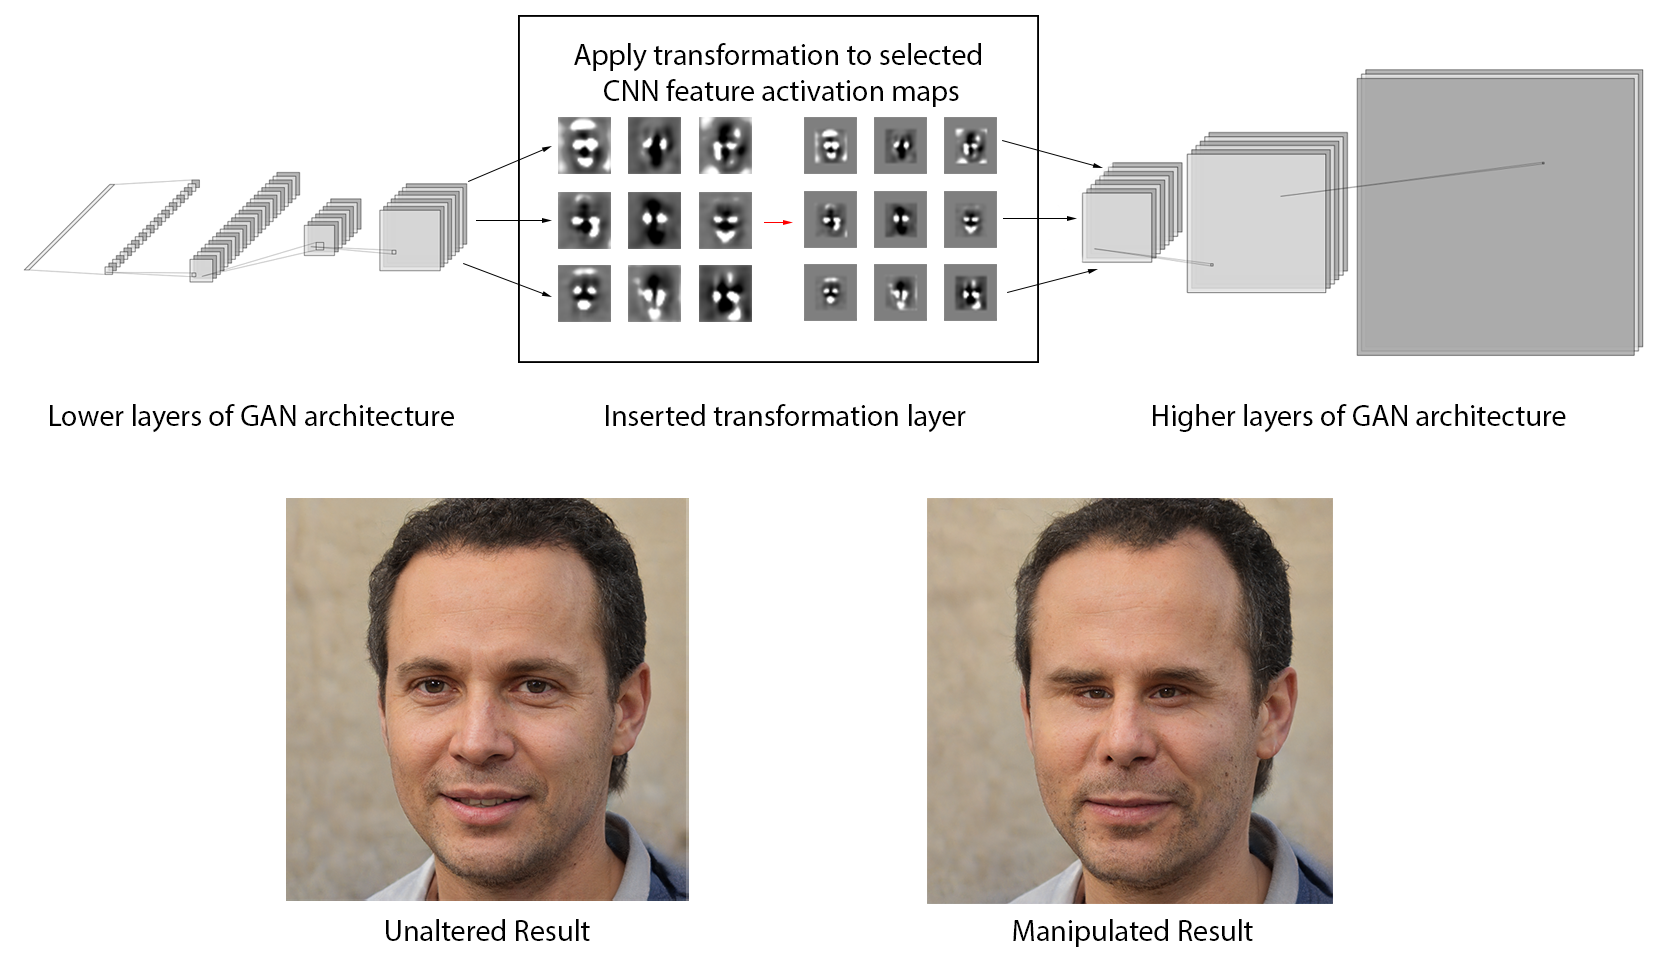
\includegraphics[width=1\textwidth]{figures/c5_netbend/misc/network-bending-diagram.png}
    \caption[Visual overview of the \textit{network bending} framework]{Visual overview of the \textit{network bending} framework, where deterministically controlled transformation layers can be inserted into a pre-trained network. As an example, a transformation layer that scales the activation maps by a factor of $k_x=k_y=0.6$ is applied (\S \ref{sec:affine}) to a set of features in layer 5 responsible for the generation of eyes, which has been discovered in an unsupervised fashion using the clustering algorithm to cluster features based on the spatial similarity of their activation maps (\S \ref{c5:sec:clustering}). Bottom left shows the sample generated by StyleGAN2 \citep{karras2019analyzing} trained on the FFHQ dataset without modification, while the image on the right shows the same sample generated with the scaling transform applied to the selected features. NB: the GAN network architecture diagram shown on the top row is for illustrative purposes only.}
    \label{fig:c5:overview_diagram}
\end{figure}

\section{Motivation}

Following the experiments detailed in Chapters \ref{ch:unstable_eq} \& \ref{ch:divergent}, I wanted to find an approach for actively diverging from data with generative neural networks, that was easier to control than methods that required the direct training or fine-tuning of the network itself.
In addition, whilst producing novel outputs, the previous approaches did not necessarily expand the possibility space of what could be generated in a way that was arguably superior to traditional generative modelling.
Both previous approaches focus on learning a set of weights that lead to reduced diversity in the generated outputs when compared with the successful training of a standard generative model such as a GAN or VAE.
The goal of the work described in this chapter was to find an approach that would expand the generative space, not shrink it. 


The inspiration for \textit{network bending} came from a conversation with my supervisor Mick Grierson.
After showing him the results detailed in the previous chapters, he said that though he liked the results, he was interested in methods that were more interactive and controllable, saying something along the lines of `I just want to stick my hand in the model and squeeze it, and see what pops out the other side' \citep{grierson2019personal}\footnote{According to Mick Grierson, the idea for network bending was also being discussed in MIMIC (Musically Intelligent Machines Interacting Creatively) research team meetings around the same time. I was not in those meetings so I cannot give an exactly chronology. However, many people clearly had similar ideas around this time as the idea of applying transformations to the activation maps of GANs was developed independently and concurrently developed by two others \citep{pinkney2020matlab,pouliot2020gan}.}. 
This statement stuck with me and eventually led to the development of the framework described here.

In some of the early experiments that led to this work, I hard-coded simple transformations into StyleGAN1 \citep{karras2019style} models during inference.
These early experiments (which later went on to become the series of artworks \textit{Teratome} \S \ref{c7:subsubsec:teratome}) sparked the intuition that eventually led to the implementation of many kinds of transformation layers (\S \ref{c5:sec:transforms}) and the clustering approach for grouping features together (\S \ref{c5:sec:clustering}).
The motivation for developing the clustering algorithm was the observation that when transformations were applied to random subsets of convolutional filters in a layer, then in some instances, manipulation of groups of filters had apparently powerful semantic effects, that could not be captured by only manipulating individual filters, as was done in the approach presented by \citep{bau2019semantic}.

In creating this framework, I wanted to give as much control and agency to people to manipulate generative neural networks as possible. 
The flexibility of this framework was key in order to achieve this, allowing for the expansion of the generative space of generative neural networks in a data-divergent fashion.

\section{Transformation Layers}

\label{c5:sec:transforms}

A key goal in this framework was to give as much direct control and agency to artists and creative practitioners as possible.
To maximise the amount of control people could have, I implemented a broad variety of deterministically controlled transformation layers that can be dynamically inserted into the computational graph of the generative model. 
The transformation layers are implemented natively in PyTorch \citep{paszke2019pytorch} for speed and efficiency. I
 treated the activation maps of each feature of the generative model as 1-channel images in the range -1 to 1. 
 Each transformation is applied to the activation maps individually before they are passed to the next layer of the network. 

 The transformation layers can be applied to all the features in a layer, or a random selection, or by using pre-defined groups automatically determined based on spatial similarity of the activation maps (\S \ref{c5:sec:clustering}). 
 Figure \ref{fig:c5:layerwide_comparison} shows a comparison of a selection of these transformations applied to all the features layer-wide in various layers of StyleGAN2.

\begin{figure}[htbp]
    \centering
    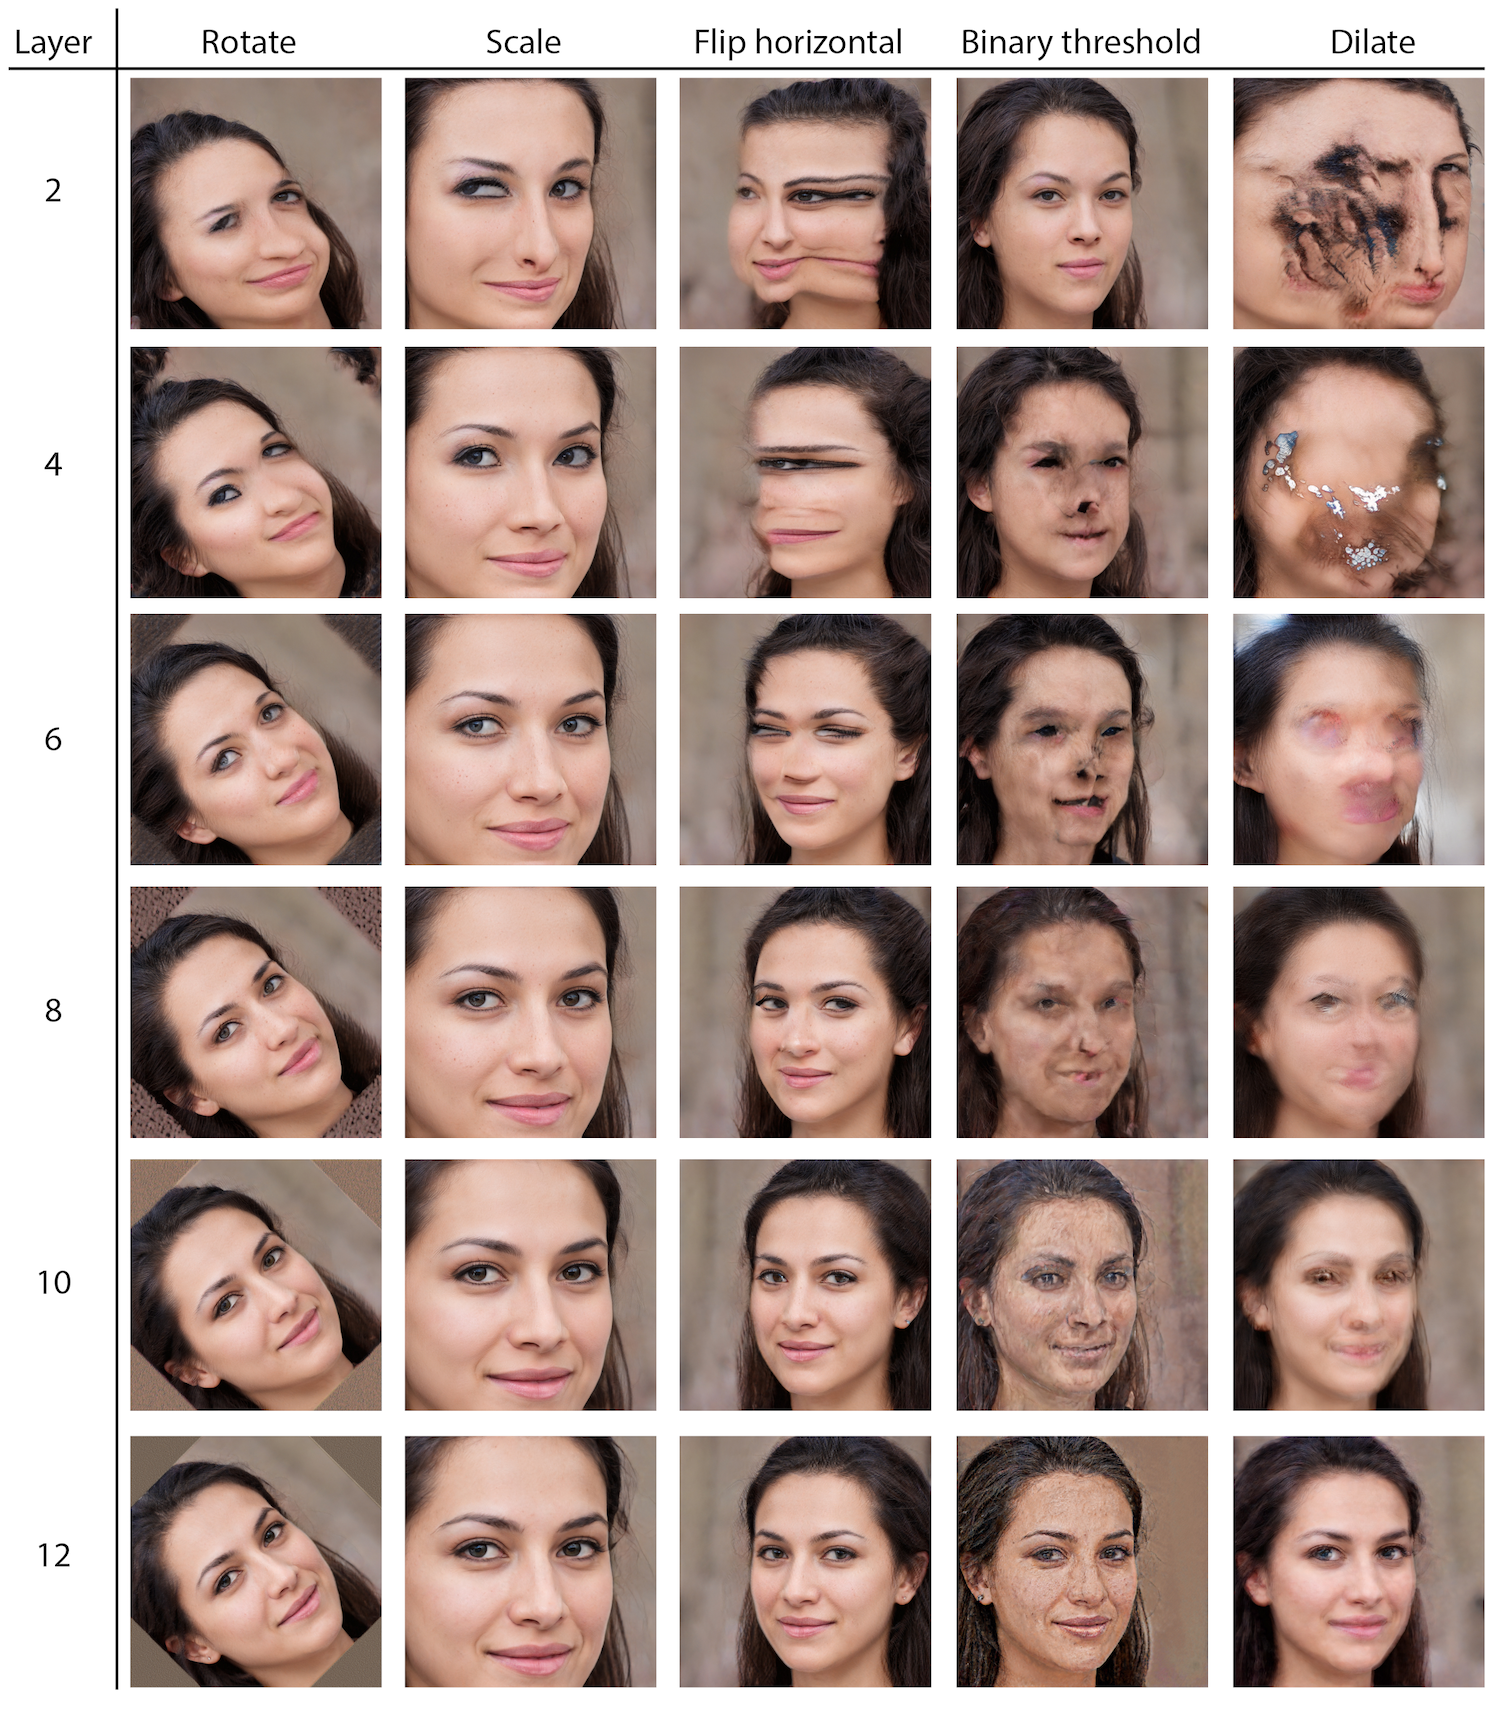
\includegraphics[width=1\textwidth]{figures/c5_netbend/misc/transform-comparison.png}
    \caption[Comparsion of various transformation layers applied in different layers of StyleGAN2]{A comparison of various transformation layers inserted and applied to all of the features in different layers in the StyleGAN2 network trained on the FFHQ dataset, showing how applying the same filters in different layers can make wide-ranging changes the generated output. The rotation transformation is applied by an angle $\theta=45$. The scale transformation is applied by a factor of $k_{x}=k_{y}=0.6$. The binary threshold transformation is applied with a threshold of $t=0.5$. The dilation transformation is applied with a structuring element with radius $r=2$ pixels.}
    \label{fig:c5:layerwide_comparison}
\end{figure}


\subsection{Pointwise Transformations}

I began with simple pointwise numerical transformations $f(x)$ that are applied to individual activation units $x$. 
I implemented four distinct numerical transformations: the first is \emph{ablation}, which can be interpreted as $f(x) = x \cdot 0$. 
The second is \emph{inversion}, which is implemented as $f(x) = 1 - x$. 
The third is \emph{multiplication by a scalar} $p$ implemented as $f(x) = x \cdot p$. 
The final transformation is \emph{binary thresholding} (often referred to  as posterisation) with threshold $t$, such that:
\begin{equation}
f(x) = \begin{cases}
    1,& \text{if  } x\geq t\\
    0,              & \text{otherwise}
\end{cases}
\end{equation}

\subsection{Affine Transformations}
\label{sec:affine}
For this set of transformations, each activation map $X$ for feature $f$ is treated as an individual matrix that simple affine transformations can be applied to. 
The first two are horizontal and vertical \emph{reflections} that are defined as:
\begin{equation}
X \begin{bmatrix}
-1 & 0 & 0\\
\ 0 & 1 & 0\\
\ 0 & 0 & 1
\end{bmatrix}\quad , \quad X \begin{bmatrix}
1 & \ 0 & 0\\
0 & -1 & 0\\
0 & \ 0 & 1
\end{bmatrix}
\end{equation}

\noindent The second is \emph{translations} by parameters $p_x$ and $p_y$ such that:
\begin{equation}
X \begin{bmatrix}
1 & 0 & p_x\\
0 & 1 & p_y\\
0 & 0 & 1
\end{bmatrix}
\end{equation}

\noindent The third is \emph{scaling} by parameters $k_x$ and $k_y$ such that:
\begin{equation}
X \begin{bmatrix}
k_x & 0 & 0\\
0 & k_y & 0\\
0 & 0 & 1
\end{bmatrix}
\end{equation}
Note that in this chapter, I only report on using uniform scalings, such that $k_x = k_y$. Finally, fourth is \emph{rotation} by an angle $\theta$ such that:
\begin{equation}
X \begin{bmatrix}
cos(\theta) & -sin(\theta) & 0\\
sin(\theta) & cos(\theta) & 0\\
0 & 0 & 1
\end{bmatrix}
\end{equation}

\subsection{Morphological Transformations}

I implemented two of the possible basic mathematical morphological transformation layers, performing \emph{erosion} and \emph{dilation} \citep{soille1999erosion} when applied to the activation maps, which can be interpreted as 1-channel images  (Fig. \ref{fig:c5:morphological transforms}). 
These can be configured with the parameter $r$ which is the radius for a circular kernel (aka structural element) used in the morphological transformations.

\begin{figure}[!htb]
    \centering
    \subfloat[]{\label{subfig:morph-a}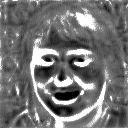
\includegraphics[width=.32\textwidth]{figures/c5_netbend/morphology_activations/original_007.png}}
    \hfill
    \subfloat[]{\label{subfig:morph-a-erode}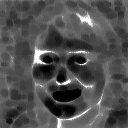
\includegraphics[width=.32\textwidth]{figures/c5_netbend/morphology_activations/erode_007.png}}
    \hfill
    \subfloat[]{\label{subfig:morph-a-dilate}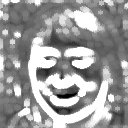
\includegraphics[width=.32\textwidth]{figures/c5_netbend/morphology_activations/dilate_007.png}}
    \caption[Examples of morphological transformations being applied to an individual activation map in Layer 10 of StyleGAN2]{Examples of morphological transformations being applied to an individual activation map in Layer 10 of StyleGAN2. (a) Unmodified activation maps. (b) Activation map after erosion was applied ($r=2$ pixels). (c) Activation maps after dilation were applied ($r=2$ pixels).}
    \label{fig:c5:morphological transforms}
 \end{figure}

\section{Clustering Features}
\label{c5:section:clustering}

As most of the layers in the current state-of-the-art generative models, such as StyleGAN2, have very large numbers of convolutional features, controlling each one individually would be far too complicated to build a user interface around and control these in a meaningful way. 
In addition, because of the redundancy existing in these models, manipulating individual features does not normally produce any kind of meaningful outcome.\footnote{I discovered this through my early hard-coded experiments with network bending that are discussed in Section \ref{c7:subsubsec:teratome}.} 
Therefore, it is necessary to find some way of grouping them into more manageable ensembles of sets of features. 
Ideally, such sets of features would correspond to the generation of distinct, semantically meaningful aspects of the image, and manipulating each set would correspond to the manipulation of specific semantic properties in the resulting generated sample. 
To achieve this, I developed a novel approach that combines metric learning and a clustering algorithm to group sets of features in each layer based on the spatial similarity of their activation maps. 
I trained a separate convolutional neural network (CNN) for each layer of StyleGAN2 to analyse the appearance of the activation maps. 
The CNN has a bottleneck architecture (first introduced by Gr{\'e}zl et al.~\citep{grezl2007probabilistic}) to learn a highly compressed feature representation; the latter is then used in a metric learning approach in combination with the $k$-means clustering algorithm \citep{lloyd1982least, celebi2013comparative} to group sets of features in an unsupervised fashion. 

\subsection{Architecture}

For each layer of StyleGAN2, I trained a separate CNN on the activation maps of all the convolutional features. 
The resolution of the activation maps and the number of convolutional features varies for the different layers of the model (a breakdown of which can be seen in Table \ref{tab:classifier-table}).
I employed an architecture that can dynamically be changed, by increasing the number of convolutional blocks, depending on what depth is required. 

\begin{table}[]
\centering
\begin{tabular}{|c|c|c|c|c|c|}%{llllll}
\hline
Layer & Resolution & \#features &  CNN depth & \#clusters & Batch size\\
\hline
1     & 8x8        & 512          & 1                & 5                & 500        \\
2     & 8x8        & 512          & 1                & 5                & 500        \\
3     & 16x16      & 512          & 2                & 5                & 500        \\
4     & 16x16      & 512          & 2                & 5                & 500        \\
5     & 32x32      & 512          & 3                & 5                & 500        \\
6     & 32x32      & 512          & 3                & 5                & 500        \\
7     & 64x64      & 512          & 4                & 5                & 200        \\
8     & 64x64      & 512          & 4                & 5                & 200         \\
9     & 128x128    & 256          & 5                & 4                & 80         \\
10    & 128x128    & 256          & 5                & 4                & 80         \\
11    & 256x256    & 128          & 6                & 4                & 50         \\
12    & 256x256    & 128          & 6                & 4                & 50         \\
13    & 512x512    & 64           & 7                & 3                & 20         \\
14    & 512x512    & 64           & 7                & 3                & 20         \\
15    & 1024x1024  & 32           & 8                & 3                & 10         \\
16    & 1024x1024  & 32           & 8                & 3                & 10       \\
\hline
\end{tabular}
\medskip
\caption[Table detailing model architecture for the ShuffleNet models used for clustering in StyleGAN2.]{
    \label{tab:classifier-table}Table showing resolution, number of features of each layer, the number of ShuffleNet \citep{zhang2018shufflenet} convolutional blocks for each CNN model used for metric learning, the number of clusters calculated for each layer using $k$-means and the batch size used for training the CNN classifiers for the StyleGAN2 models. Note: LSUN church and cat models have only 12 layers.
%\citep{lloyd1982least, celebi2013comparative}.
}
\end{table}

I employed the ShuffleNet architecture \citep{zhang2018shufflenet} for the convolutional blocks in the network. 
For each convolutional block, I utilised a feature depth of 50 and had one residual block per layer. 
The motivating factor in many of the decisions made for the architecture design was not focused on achieving the best accuracy per se. 
Instead, I wanted a network that could learn a sufficiently good metric while also being reasonably quick to train (with 12-16 separate classifiers required to be trained per the StyleGAN2 model). 
I also wanted a lightweight enough network, such that it could be used in a real-time setting where clusters can quickly be calculated for an individual latent encoding, or when processing large batches of samples.

After the convolutional blocks, I flattened the final layer and used this to learn a mapping into a narrow bottleneck $\vec{v} \in \mathbb{R}^{10}$, before re-expanding the dimensionality of the final layer to the number of convolutional features present in the layer of the respective generative model. 
The goal of this bottleneck is to force the network to learn a highly compressed representation of the different convolutional features in the generative model. 
While this invariably loses some information, most likely negatively affecting classification performance during training, this is in fact the desired result. 
I wanted to force the CNN to combine features of the activation maps with similar spatial characteristics so that they can easily be grouped by the clustering algorithm. 
Another motivating factor is that the chosen clustering algorithm ($k$-means) does not scale well for feature spaces with high dimensionality.

\subsection{Training}

I generated a training set of the activations of every feature for every layer of 1000 randomly sampled images and a test set of 100 samples for the models trained on all of the datasets used in these experiments. 
I trained each CNN using the softmax feature learning approach \citep{dosovitskiy2014discriminative}, a reliable method for distance metric learning. This method employs the standard softmax training regime \citep{bridle1990probabilistic} for CNN classifiers. 
Each classifier has been initialised with random weights and then trained for 100 epochs using the Adam optimiser \citep{kingma2015adam} with a learning rate of 0.0001 and with $\beta_1 = 0.9$ and $\beta_2 = 0.999$. 
All experiments were carried out on a single NVIDIA GTX 1080ti. The batch size used for training the classifiers for the various layers of StyleGAN2 can be seen in Table \ref{tab:classifier-table}. 
% The classifiers for the VAE were all trained with a batch size of 100.

After training, the softmax layer is discarded and the embedding of the bottleneck layer is used as the discriminative feature vector where the distances between points in feature space permit gauging the degree of similarity of two samples. 
This approach differs from standard softmax feature learning as it uses the feature vector from the bottleneck, rather than the last layer prior to softmax classification, giving a more compressed feature representation than the standard softmax feature learning approach.

\subsection{Clustering Algorithm}

\label{c5:sec:clustering}

Once each of the CNNs for every layer has been trained, they can then be used to extract feature representations of the activation maps of the different convolutional features corresponding to each layer of the generative model.
The approach is to perform clustering based on an average of features' embeddings drawn from many random samples, which can be used to find a general-purpose set of clusters for a trained model.

The activation map $X_{df}$ for each layer $d$ and feature $f$ is fed into the CNN metric learning model for that layer $C_d$ to get the feature vector $\vec{v}_{df}$. 
This process is repeated N times (1000 in these experiments) to find the mean feature vector $\vec{\bar{v}}_{df}$ for each convolutional filter.
The mean feature vectors for each filter in each layer are then aggregated and fed to the $k$-means clustering algorithm --- using Lloyd's method \citep{lloyd1982least} with Forgy initialization \citep{forgy1965cluster, celebi2013comparative}. 

The predetermined number of clusters for each layer in StyleGAN2 can be seen in Table \ref{tab:classifier-table}. 
Examples from the clustering algorithm applied to the FFHQ StyleGAN2 model can be seen in Figure \ref{fig:c5:cluster_layer_comp_image}.

\begin{figure}[!htbp]
    \centering
        \subfloat[]{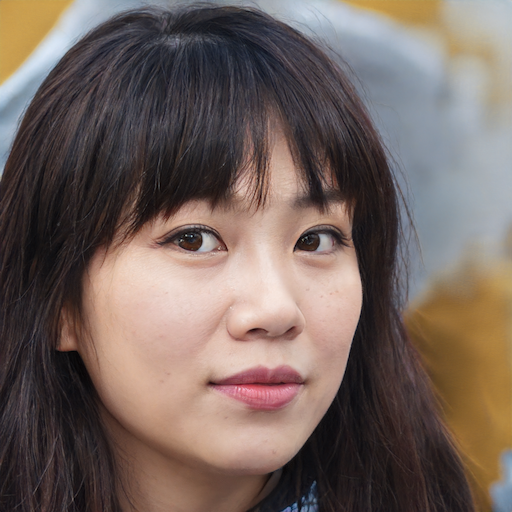
\includegraphics[width=.24\textwidth]{figures/c5_netbend/cluster_comparison/not_manipulated.png}}
        \hfill
        \subfloat[]{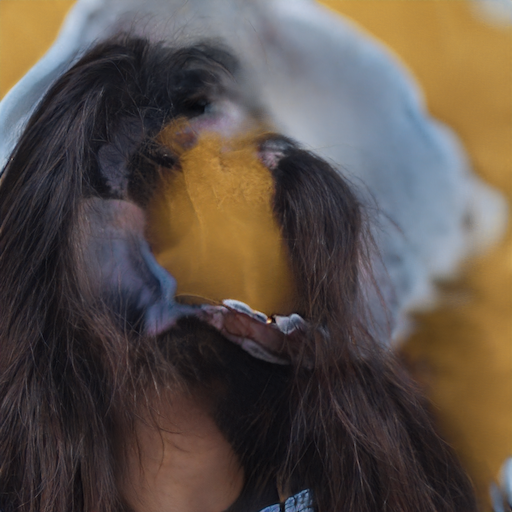
\includegraphics[width=.24\textwidth]{figures/c5_netbend/cluster_comparison/layer_1_cluster0_mult-1.png}}
        \hfill
        \subfloat[]{
\includegraphics[width=.24\textwidth]{figures/c5_netbend/cluster_comparison/layer_3_cluster2_mult5.png}}
        \hfill
        \subfloat[]{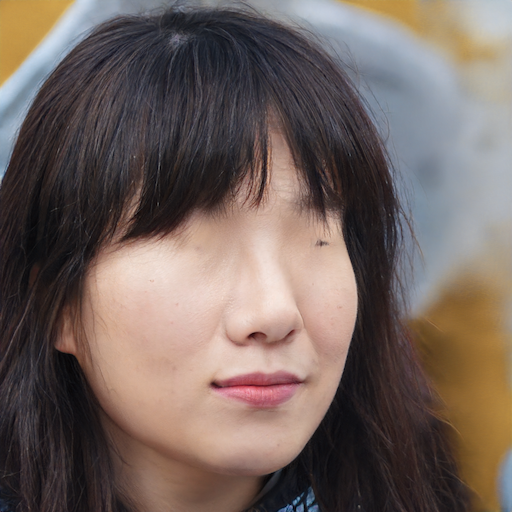
\includegraphics[width=.24\textwidth]{figures/c5_netbend/cluster_comparison/layer_5_cluster2_ablate.png}}
        \hfill
        \subfloat[]{ 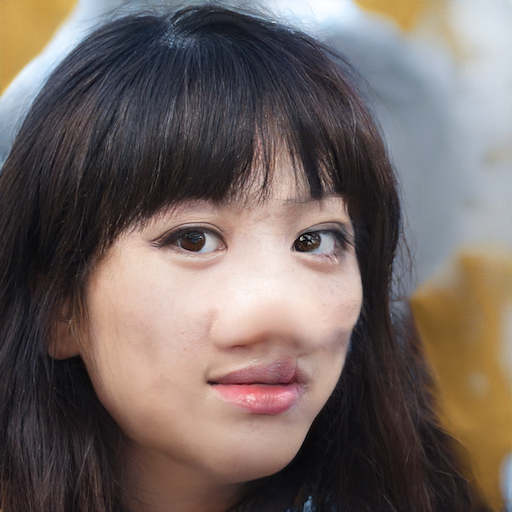
\includegraphics[width=.24\textwidth]{figures/c5_netbend/cluster_comparison/layer_6_cluster4_dilate.png}}
        \hfill
        \subfloat[]{ 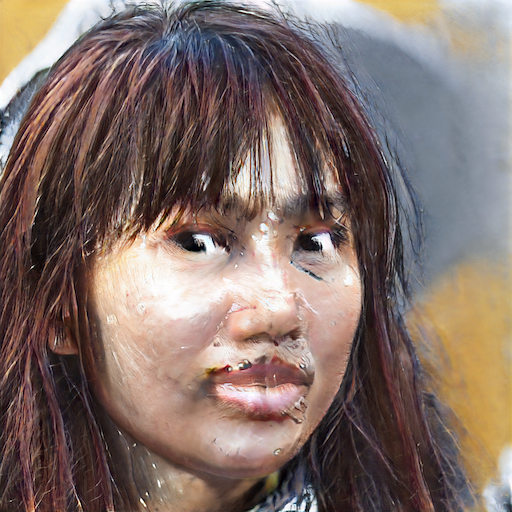
\includegraphics[width=.24\textwidth]{figures/c5_netbend/cluster_comparison/layer_9_cluster3_mult5.png}}
        \hfill
        \subfloat[]{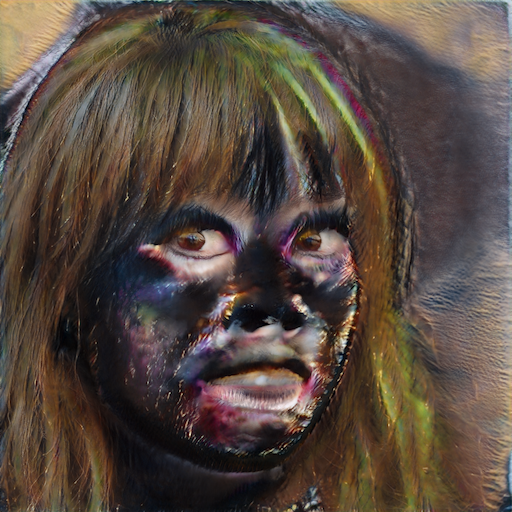
\includegraphics[width=.24\textwidth]{figures/c5_netbend/cluster_comparison/layer_10_cluster0_mult-1.png}}
        \hfill
        \subfloat[]{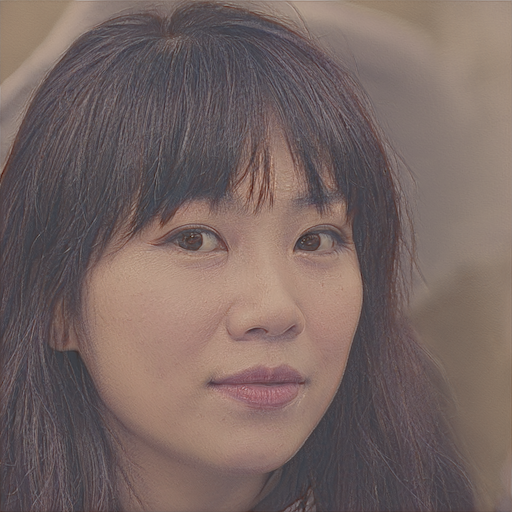
\includegraphics[width=.24\textwidth]{figures/c5_netbend/cluster_comparison/layer_15_cluster0_mult0.1.png}}
       \caption[A comparison of different transforms being applied to different clusters in various layers of StyleGAN2]{Examples from the clustering algorithm in the image domain. Clusters of features in different layers of the model are responsible for the formation of different image attributes. (a) The unmanipulated result. (b) A cluster in layer 1 has been multiplied by a factor of -1 to completely remove the facial features. (c) A cluster in layer 3 has been multiplied by a factor of 5 to deform the spatial formation of the face. (d) A cluster in layer 6 has been ablated to remove the eyes. (e) A cluster in layer 6 has been dilated with a structuring element with radius $r=2$ pixels to enlarge the nose. (f) A cluster in layer 9 has been multiplied by a factor of 5 to distort the formation of textures and edges. (g) A cluster of features in layer 10 has been multiplied by a factor of -1 to invert the highlights on facial regions. (h) A cluster of features in layer 15 has been multiplied by a factor of 0.1 to desaturate the image. All transformations have been applied to sets of features discovered using the feature clustering algorithm (\S \ref{c5:section:clustering}) in the StyleGAN2 model trained on the FFHQ dataset.}
       \label{fig:c5:cluster_layer_comp_image}
    \end{figure}

The main motivation of the clustering algorithm presented in this paper was to simplify the parameter space in a way that allows for more meaningful and controllable manipulations whilst also enhancing the expressive possibilities afforded by interacting with the system. 
These results show that the clustering algorithm is capable of discovering groups of features that correspond to the generation of different semantic aspects of the results, which can then be manipulated in tandem. 
These semantic properties are discovered in an unsupervised fashion and across the entire hierarchy of features present in the generative model.
Figure \ref{fig:c5:cluster_layer_comp_image} shows the manipulation of groups of features across a broad range of layers that control the generation of the entire face, the spatial formation of facial features, the eyes, the nose, textures, facial highlights and overall image contrast.

\section{Manipulation Pipeline}

Transforms are specified in YAML (YAML Ain't Markup Language) configuration files \citep{ben2009yaml} (Fig. \ref{fig:c5:yaml-transform-config} for an example of one of these configs), such that each transform is specified with 5 items: (i) the layer, (ii) the transform itself, (iii) the transform parameters, (iv) the layer type (i.e. how the features are selected in the layer: across all features in a layer, to pre-defined clusters, or to a random selection of features), and (v) the parameter associated with the layer type (either the cluster index, or the percentage of features the filter will randomly be applied to). 
Visual examples of how different layer types can be seen in Figure \ref{fig:c5:layer-transform-types}.
There can be any number of transforms defined in such a configuration file and transforms can be chained together to produce more complex filtering effects in the generated output  (Fig. \ref{subfig:chaining-transformations}).

After loading the configuration, the software either looks up which features are in the cluster index or randomly applies indices based on the random threshold parameter. 
Then the latent is loaded, which can either be randomly generated, or be predefined in latent space $z$, or be calculated using a projection in latent space $w$ \citep{abdal2019image2stylegan,karras2019analyzing} (in the case of StyleGAN2). The latent code is provided to the generator network and inference is performed. 
As this implementation uses PyTorch \citep{paszke2019pytorch}, a dynamic neural network library, these transformation layers can therefore be inserted dynamically during inference as and when they are required and applied only to the specified features as defined by the configuration. 
Once inference is unrolled, the generated output is returned. Figure \ref{fig:c5:overview_diagram} provides a visual overview of the pipeline, as well as a comparison between a modified and unmodified generated sample.

\begin{figure}[!htb]
    \centering
    \subfloat[]{\label{subfig:layer-wide}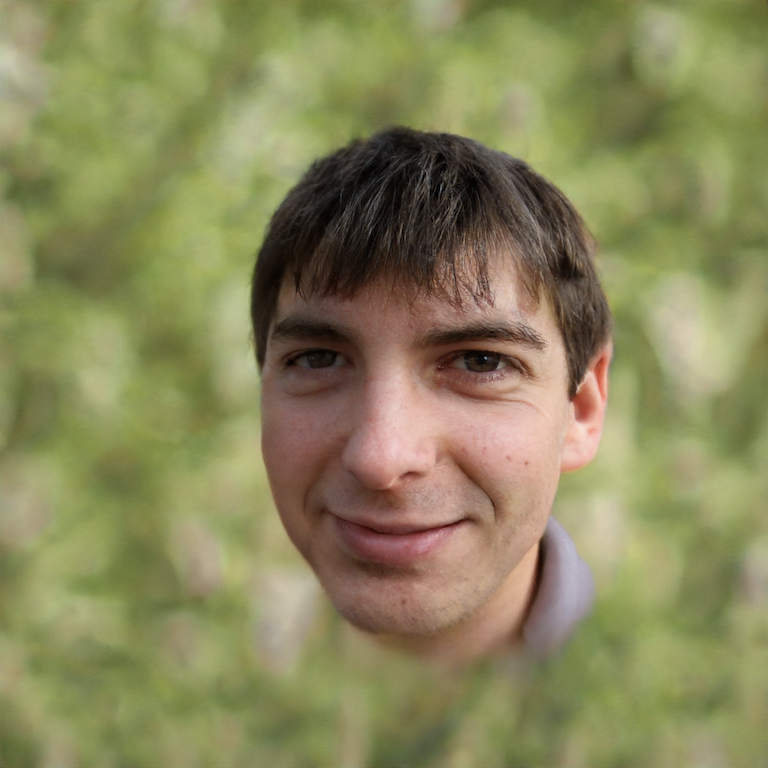
\includegraphics[width=.24\textwidth]{figures/c5_netbend/layer-transform-types/layer-wide.png}}
    \hfill
    \subfloat[]{\label{subfig:random-layer}
\includegraphics[width=.24\textwidth]{figures/c5_netbend/layer-transform-types/stochastic.png}}
    \hfill
    \subfloat[]{\label{subfig:cluster-layer}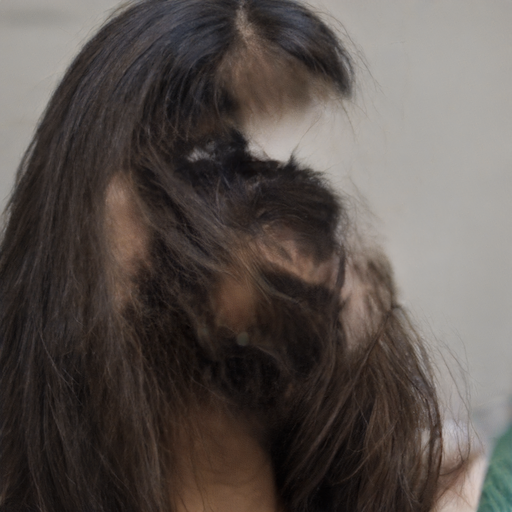
\includegraphics[width=.24\textwidth]{figures/c5_netbend/layer-transform-types/cluster.png}}
    \hfill
    \subfloat[]{\label{subfig:chaining-transformations}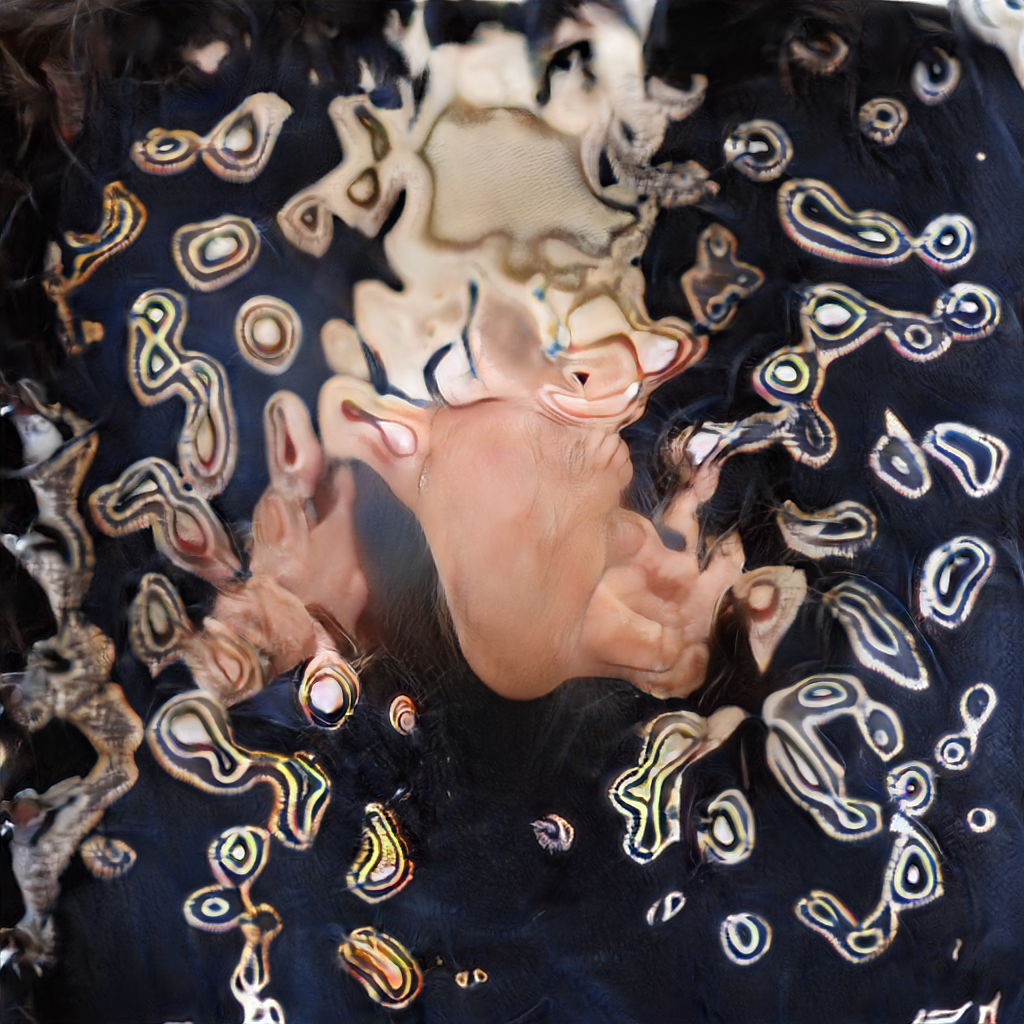
\includegraphics[width=.24\textwidth]{figures/c5_netbend/layer-transform-types/chaining-transforms.png}}
    \caption[Examples of transformation layers being applied to different configurations of features]{Examples of transformation layers being applied to different configurations of features in StyleGAN2. (a) Transformation applied layer-wide. (b) Transformation is applied to a random selection of filters in one layer. (c) Transformation applied to a cluster in layer 2. (d) A combination of transformation layers applied across a network, the configuration of transformations used to generate this image can be seen in Figure \ref{fig:c5:yaml-transform-config}.}
    \label{fig:c5:layer-transform-types}
 \end{figure}

 \begin{figure}[!htb]
 \begin{lstlisting}[language=yaml]
    ---
    transforms:
    - layer: 2
      transform: "invert"
      params: []
      features: "all"
      feature-param: 
    - layer: 6
      transform: "binary-thresh"
      params: [0.5]
      features: "random"
      feature-param: 0.5
    - layer: 6
      transform: "scalar-multiply"
      params: [5]
      features: "cluster"
      feature-param: 2
    ---
    \end{lstlisting}
    \caption[Example YAML transformation config]{Example of a YAML transformation config that is used in the network bending framework. This config combines randomly applied layers and layer-wide transformations. This config was used to generate the image Figure \ref{subfig:chaining-transformations}.}
    \label{fig:c5:yaml-transform-config}
 \end{figure}

\section{Network Bending in the Audio Domain}
\label{c5:sec:net-bend-audio}

As a follow-up study to the original network bending approach on images, I applied the same approach to the audio domain as an extension to the work for the journal paper in Entropy \citep{broad2022network}. 
The motivation for this was to demonstrate that network bending was applicable to different types of media and to demonstrate the general-purpose nature of this framework. 

For this study, I trained a custom VAE model on spectrograms of music and applied the exact same algorithm for clustering and applying the same transformation layers as was applied in network bending for image generation. 
Network bending has also been applied to audio by other researchers and practitioners, this efforts are detailed in Sections \ref{c7:subsubsec:naotokui} \& \ref{c7:subsubsec:ddsp}.

\subsection{Custom Audio Model}

For this experiment, I trained a variational autoencoder (VAE) \citep{kingma2013auto,rezende2014stochastic} on spectrograms extracted from a custom dataset of varied musical genres, totalling 3461 audio tracks. This approach is based on previous methods for learning generative models of spectrograms \citep{akten2018granma} and Mel spectrograms \citep{valenzuela2021melspecvae} with VAEs. The tracks are randomly split up into short sequences and the Fourier transform is performed with a hop size of 256 and a window size of 1024 to produce spectrograms that have a bin size of 513. The spectrograms are then cut into shorter sequences of a window length of 128. These shortened spectrograms are then converted to decibels and then normalised for training with the VAE.  

The VAE was built using a convolutional architecture with a latent vector with dimension $\vec{v} \in \mathbb{R}^{512}$. The encoder has 5 layers that use standard convolutions with a kernel size of 5x5, a stride of 2x2 and no padding for all of the layers. The decoder uses transposed convolutions, and Table \ref{tab:c5:decoder-architecture} lists the output resolution, kernel size, stride, and padding parameters for each of the 5 convolutional layers. A fully connected layer is used in both the encoder and decoder to interface between the convolutional layers and the latent vector. The model was trained for 50 epochs on the dataset with batch normalisation using a batch size of 64. The model was trained using the Adam optimiser \citep{kingma2014adam} with a learning rate of 0.0003 and with $\beta_1 = 0$ and $\beta_2 = 0.99$.

After training it is possible to sample randomly in the latent space and then sample directly from the decoder. It is also possible to input audio sequences, both from the training set and outside of it, and produce reconstructions of the audio track mediated through the VAE model, in a method that I have previously referred to as \textit{autoencoding} \citep{broad2017autoencoding}. Performing this autoencoding procedure in combination with network bending, provides a new way of transforming and filtering audio.

\begin{table*}[]
    \centering
    \begin{tabular}{|c|c|c|c|c|c|c|c|}
    \hline
    Layer & Resolution & \#features & kernel size & stride & padding \\
    \hline
    1     & 8x33       & 512        & 5x5         & 1x2     & 0x2  \\
    2     & 17x65      & 256        & 3x5         & 2x2     & 2x2 \\
    3     & 32x129     & 128        & 4x5         & 2x2     & 2x2 \\
    4     & 64x257     & 64         & 4x5         & 2x2     & 2x2  \\
    5     & 128x513    & 1          & 4x5         & 2x2     & 2x2  \\
    \hline
    \end{tabular}
    \medskip
    \caption{\label{tab:c5:decoder-architecture}Table showing resolution, number of features of each layer, convolutional kernel size, strides, and padding parameters for the decoder network in the spectrogram VAE.}
    
    \end{table*}

\subsection{Clustering}

the approach to clustering for this audio model was identical to what was demonstrated in Section \ref{c5:section:clustering}.
As the VAE model did not have as many layers as StyleGAN2, clusters were only calculated for four layers, the details of which can be seen in Table \ref{tab:c5:audio-clustering}.

\begin{table*}[]
    \centering
    \begin{tabular}{|c|c|c|c|c|c|c|c|}
    \hline
    Layer & CNN Depth & \#clusters \\
    \hline
    1     & 1 &   5 \\
    2     & 2 &   5 \\
    3     & 3 &   4 \\
    4     & 4 &  4 \\
    \hline
    \end{tabular}
    \medskip
    \caption{\label{tab:c5:audio-clustering}Table showing the number of ShuffleNet \citep{zhang2018shufflenet} convolutional blocks for each CNN model used for metric learning and the number of clusters calculated for each layer using $k$-means.}
    
    \end{table*}

\subsection{Results}

The clustering approach applied to the audio model appears to work well when visualising the spectrograms, and it is clear that this approach can capture and manipulate some semantically meaningful components in the audio signal\footnote{Unfortunately there was a bug in the decoding of the spectrograms back into audio which meant that the audio quality in the generated samples was very noisy -- something that I have not been able to fix.}  (Fig. \ref{fig:c5:cluster_audio_comp}). 
Not all of the transformations that can be applied to images work as well in audio, such as scaling and rotation.
This is not a surprise given that the location of each pixel is essential information used to represent frequency and time information in the audio signal, and can completely transform the information represented when manipulated.
However, the morphological transformations do at least preserve locality in the signal, and using these filters in generative models of spectrograms offers a completely new way to transform audio signals.

\begin{figure}[tp!]
\vspace{-80pt}
\centering
    \subfloat[]{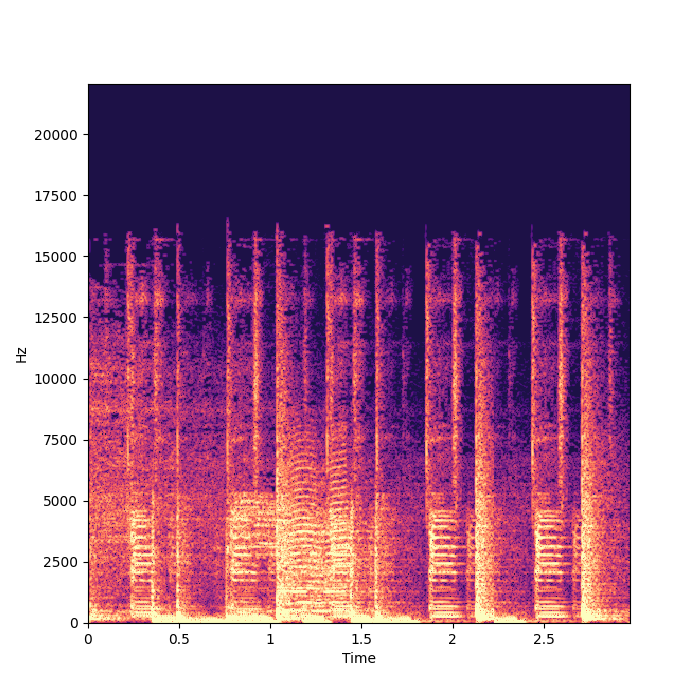
\includegraphics[width=.4\textwidth]{figures/c5_netbend/audio_clusters/soul_short_original.png}}
    \hfill
    \subfloat[]{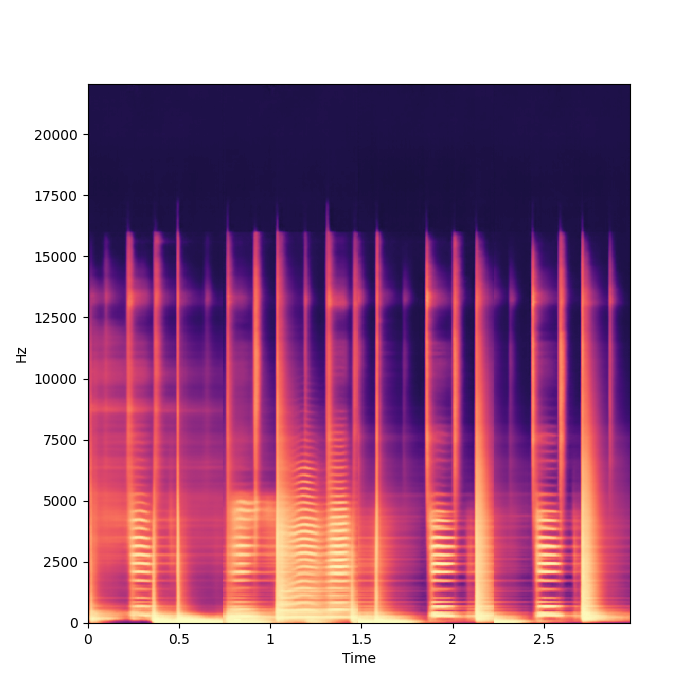
\includegraphics[width=.4\textwidth]{figures/c5_netbend/audio_clusters/soul_short_reconstruction.png}}
   \hfill
    \subfloat[]{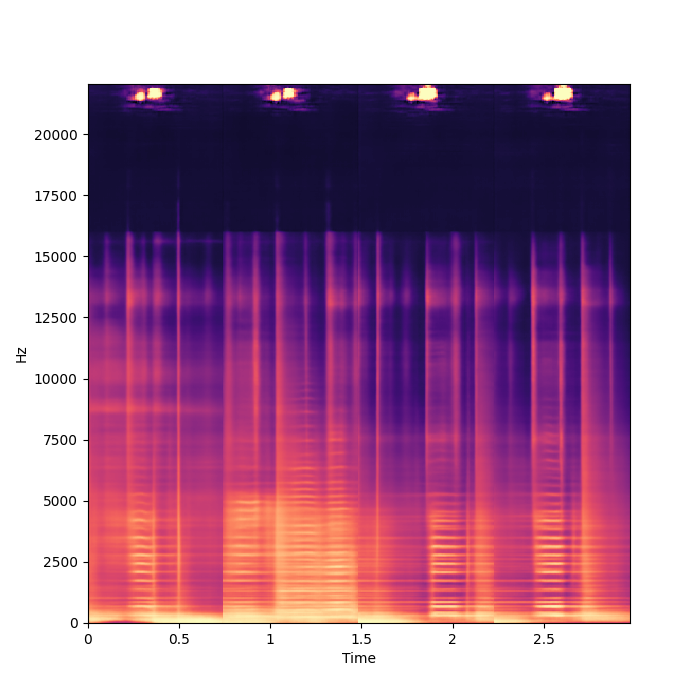
\includegraphics[width=.4\textwidth]{figures/c5_netbend/audio_clusters/layer_1_cluster3_ablate.png}}
    \hfill
    \subfloat[]{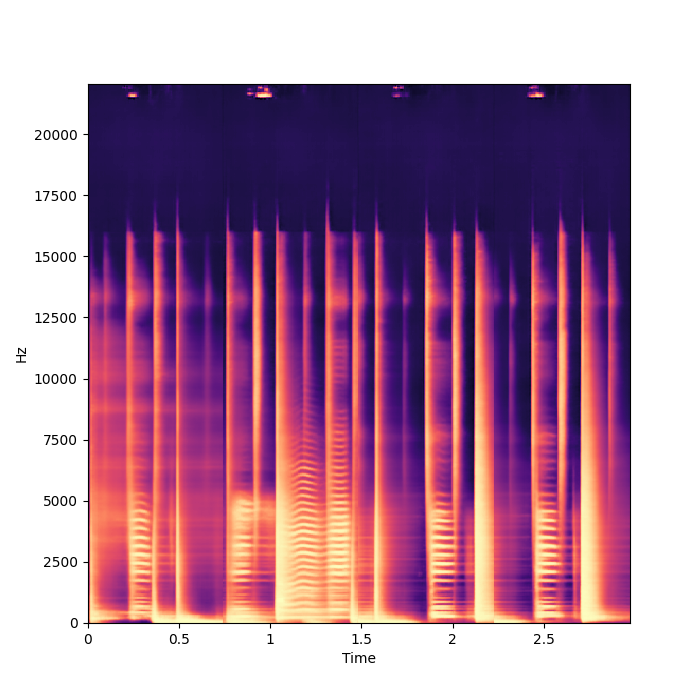
\includegraphics[width=.4\textwidth]{figures/c5_netbend/audio_clusters/layer_1_cluster3_mult_2.png}}
   \hfill
    \subfloat[]{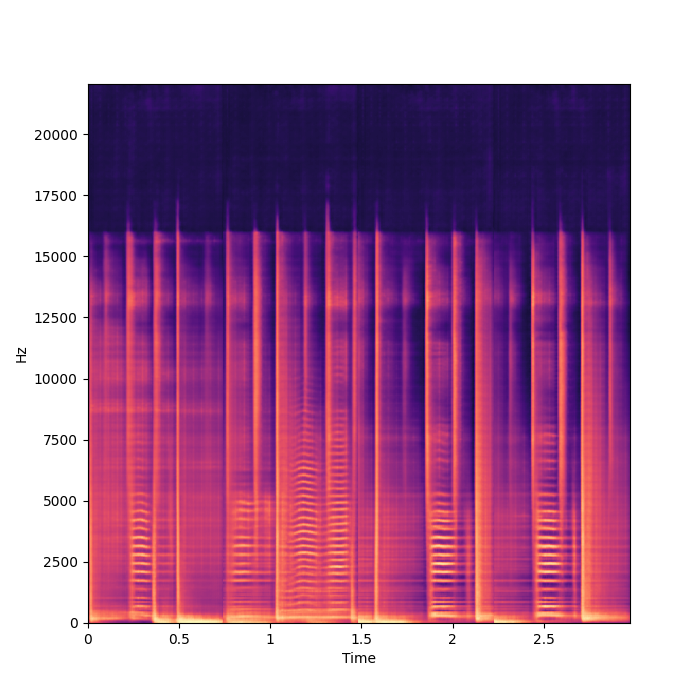
\includegraphics[width=.4\textwidth]{figures/c5_netbend/audio_clusters/layer_3_cluster2_erode.png}}
    \hfill
    \subfloat[]{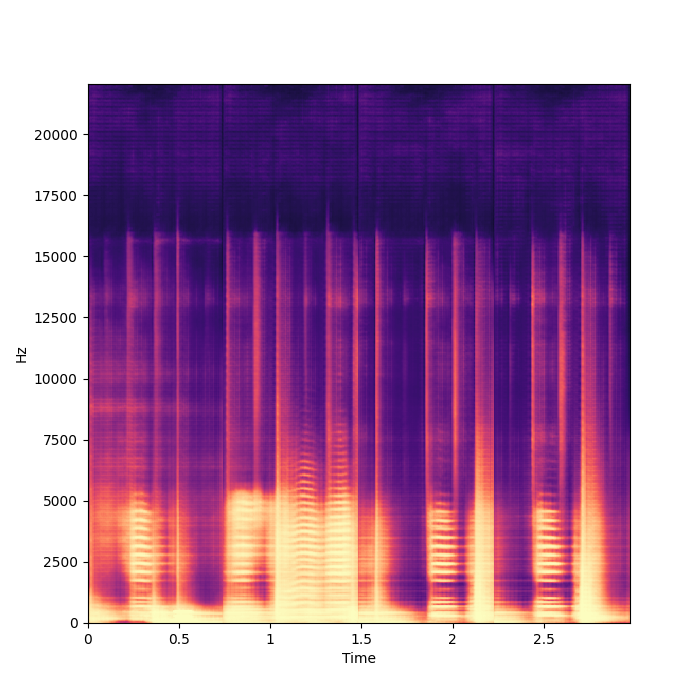
\includegraphics[width=.4\textwidth]{figures/c5_netbend/audio_clusters/layer_3_cluster2_dilate.png}}
   \caption[A comparison of different transforms being applied to different clusters in various layers of the SpectrogramVAE]{Examples from the clustering approach in the audio domain. (a) Spectrogram of an original source track not in the training set. (b) Reconstruction of source track using VAE without manipulation. (c) Reconstruction of the same signal where a cluster in layer 1 responsible for the generation of the transients of the signal has been ablated. (d) Reconstruction of the same signal where the same cluster in layer 1 responsible for the transients has been multiplied by a factor of 2, increasing the intensity of the transients in the resulting signal. (e) Reconstruction of the signal where a cluster in layer 3 responsible for the low and mid-range frequencies has been eroded with a structuring element with radius $r=2$ pixels, diminishing the intensity of these frequency components. (f) Reconstruction of the signal where the same cluster in layer 3 responsible for the low and mid-range frequencies has been dilated with a structuring element with radius $r=2$ pixels, increasing the intensity of these frequency components. The audio sample used is a clip from \textit{Saulsalita Soul} by Mr.RuiZ, reproduced and transformed with permission granted under the CC BY-NC 4.0 licence.}
   \label{fig:c5:cluster_audio_comp}
\end{figure}

\section{Discussion}

In this section, I discuss several different perspectives on the outcomes presented here: expressive manipulation, active divergence, comparisons of the results between the image and audio domains, and comparisons with other methods.

\subsection{Expressive Manipulation}

The main motivation of the clustering algorithm presented in this chapter was to simplify the parameter space in a way that allows for more meaningful and controllable manipulations whilst also enhancing the expressive possibilities afforded by interacting with the system. 
These results show that the clustering algorithm is capable of discovering groups of features that correspond to the generation of different semantic aspects of the results, which can then be manipulated in tandem. 
These semantic properties are discovered in an unsupervised fashion and across the entire hierarchy of features present in the generative model.
For example, Figure \ref{fig:c5:cluster_layer_comp_image} shows the manipulation of groups of features across a broad range of layers that control the generation of the entire face, the spatial formation of facial features, the eyes, the nose, textures, facial highlights and overall image contrast. Figure \ref{fig:c5:cluster_audio_comp} shows the clustering algorithm performed in the audio domain, to demonstrate how aspects of the audio signal such as the transients and frequency components can be manipulated with various kinds of transformations.

Grouping and manipulating features in a semantically meaningful fashion is an important component of allowing expressive manipulation. 
However, artists are often also ready to consider surprising, unexpected results, to allow for the creation of new aesthetic styles, which can become uniquely associated with an individual or group of creators. 
Therefore the tool needs to allow for unpredictable as well as predictable possibilities, which can be used in an exploratory fashion and can be mastered through dedicated and prolonged use \citep{dobrian2006nime}. 
There is usually a balance between the utility and expressiveness of a system \citep{jacobs2017supporting}. 

Section \ref{c7:sec:net-bend-artworks} shows the various different ways this framework has been used to make artworks.
Whilst I did not make a user interface for network bending myself, many other researchers have gone on to do so.
Their efforts are detailed in Section \ref{c7:subsec:net-bend-interfaces}.

\subsection{Comparison Between Audio and Image Domains}

In this chapter, I have described the network bending framework in both the image and audio domains. 
For the image domain, I have used StyleGAN2 \citep{karras2019analyzing}, the state of the art generative model for unconditional image generation. In the audio domain, I have built a custom generative model to demonstrate how the same principles of clustering features and applying transformations to clustered features can be applied indirectly to another domain. 
The generative model for audio I have presented is building on a much smaller body of research and has more room for improvement in terms of the fidelity of the generated outputs, however, it is still adequate and demonstrates that the clustering algorithm is capable of discovering semantically meaningful components of the signal  (Fig. \ref{fig:c5:cluster_audio_comp}). 
Some of the transformation layers that were designed for image-based models such as rotation and scaling do not transfer meaningfully into the audio domain. 
However, numerical and morphological transformations do work effectively in the audio domain, representing a completely new approach for manipulating audio signals. 
In addition to my efforts, other researchers have also gone on to successfully implement network bending in audio models (\S \ref{c7:subsubsec:naotokui} \& \S \ref{c7:subsubsec:ddsp}).

\subsection{Comparison with Other Methods}

With respect to the semantic analysis and manipulation of a generative model, this approach of clustering features and using a broad array of transformation layers is a significant advance over previous works \citep{Bau2017-vg,Bau2018-td,bau2019semantic, Brink2019-gc}. 
This recent thread of techniques only interrogates the function of individual features, and as such is unlikely to be capable of capturing a full account of how a deep network generates results since such networks tend to be robust to the transformation of individual features. 

The results in this chapter show that sets of features, which may not be particularly responsive to certain transformations, are very responsive to others. 
Figure \ref{fig:c5:ablation_comp} shows that in the model trained on the LSUN church dataset, a cluster of features, when ablated, have little noticeable effect on the result.
However, significant changes are visible when using the pointwise scalar multiplication transformation on the same cluster, here removing the trees and revealing the church building that was obscured by the foliage in the original result. 
The clustering approach described in this paper suggests that the functionality of features, or sets of features, cannot be understood only through ablation, because of the high levels of redundancy present in the learned network parameters. 
In addition, the research here shows that their functionality can be better understood by applying a wide range of deterministic transformations, of which different transformations, some of which are better suited to revealing the utility of different sets of features (Figs. \ref{fig:c5:cluster_layer_comp_image} \& \ref{fig:c5:ablation_comp}). 
An approach that has since been developed further by \cite{oldfield2022panda,oldfield2024bilinear}.

\begin{figure}[!htbp]
   \centering
   \subfloat[]{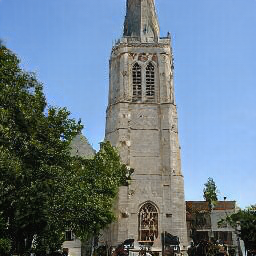
\includegraphics[width=.32\textwidth]{figures/c5_netbend/church_ablation_comparison/not_manipulated.png}}
   \hfill
   \subfloat[]{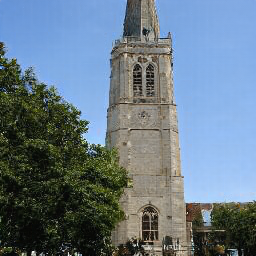
\includegraphics[width=.32\textwidth]{figures/c5_netbend/church_ablation_comparison/layer_3_cluster1_ablate.png}}
   \hfill
   \subfloat[]{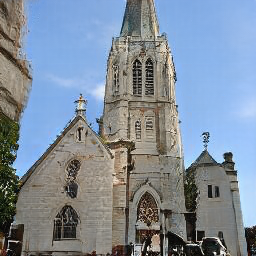
\includegraphics[width=.32\textwidth]{figures/c5_netbend/church_ablation_comparison/layer_3_cluster1_mult5.png}}
   \caption[A comparison of one cluster in StyleGAN2 having two different transforms applied to it]{Groups of features that are not particularly sensitive to ablation may be more sensitive to other kinds of transformation. (a) Original unmodified input. (b) A cluster of features in layer 3 that has been ablated. (c) The same cluster of features that has been multiplied by a scalar of 5. As can be seen, ablation had a negligible effect, only removing a small roof structure that was behind the foliage. On the other hand, multiplying by a factor of 5 removes the trees whilst altering the building structure to have gable roof sections on both the left and right sides of the church - which are now more prominent and take precedence in the generative process. Samples are taken from the StyleGAN2 model trained on the LSUN church dataset.}
   \label{fig:c5:ablation_comp}
\end{figure}

This method of analysis is completely \emph{unsupervised} and does not rely on auxiliary models trained on large labelled datasets (such as in \citep{Bau2018-td, isola2017image, park2019semantic}) or other kinds of domain-specific knowledge. 
This approach therefore can be applied to any CNN-based generative model architecture which has been trained on any dataset, as I have demonstrated by using the exact same clustering method for both image and audio domains. 
This is of particular relevance to artists who create their own datasets and would want to apply these techniques to models they have trained on their own data. 
Labelled datasets are prohibitively time-consuming (and expensive) to produce for all but a few individuals or organisations. 
Having a method of analysis that is completely unsupervised and can be applied to unconditional generative models is important in opening up the possibility for such techniques to become adopted more broadly.
Section \ref{c7:sec:net-bend-artworks} details a number of artworks made by myself and others, applied to a range of datasets, both preexisting and custom.
The limitation of this approach is the time and computational resources needed to train a separate model for each layer of the network.
This limitation is discussed further in Section \ref{c9:sec:limitations}, and ways to improve upon this are further presented in Section \ref{c9:sec:future}.


\section{Conclusion}

In this chapter, I have introduced a novel approach for the interaction with and manipulation of generative neural networks, which has been demonstrated in both the image and audio domains. 
By inserting deterministic filters inside pre-trained neural networks, this framework allows for manipulation to be performed inside the networks' `black-box', generating samples that have no resemblance to the training data, or anything that could be created easily using conventional media editing software. 
This chapter also presents a novel clustering algorithm that can group sets of features in an unsupervised fashion, based on the spatial similarity of their activation maps. 
I have demonstrated that this method is capable of finding sets of features that correspond to the generation of a broad array of semantically significant aspects of the generated results in both image and audio domains. 

The goal of the work in this thesis was to find a way to expand the possibility space of what can be generated with neural networks.
\textit{Network bending} is an approach that expands the generative space of existing pre-trained models in a way that gives direct control and agency to artists and creative practitioners, and in a way that \textit{actively diverges} from data.
This now concludes the documentation of new algorithms and approaches to \textit{active divergence} presented in this thesis. 
The next chapter will a broader perspective, contextualising the work in this thesis with other related efforts that occurred during its development.
Chapter \ref{ch:active_div} gives a detailed survey and taxonomy of active divergence methods, placing the work presented in this thesis into a larger context and delineating and outlining the landscape of active divergence methods to date. 


\chapter*{Interlude}
\addcontentsline{toc}{chapter}{Interlude}
\label{ch:interlude}



\chapter{Impact}
\label{ch:impact}

\section{Introduction}

This chapter details the impact the work described in this thesis has had, including outcomes like artworks that were made by myself and others; recognition, such as exhibitions and awards. 
This also includes an overview of work and research that follows and has been influenced by this research, applications of the research into other domains, and examples of ideas from this thesis being used and put into technologies and practical interfaces. 

\section{\textit{(un)stable equilibrium}}

As a direct outcome of the experiments detailed in Chapter 3, a series of six video artworks titled (un)stable equilibrium 1:1, 1:2, … 1:6 were made by sampling from the paired generative models, in-parallel, using the same latent code. 
A looping spherical interpolation \citep{white2016sampling} of the two videos was produced, which lasted approximately one hour. 
The interpolations were deliberately designed to be slow to provide a meditative loop seamlessly so that it could be played in a gallery setting without any interruption.

\textbf{Figure: Show a sample of the work here}

The works were first shown in the exhibitions for the respective conferences ICCV and NeurIPS in 2019. 
At NeurIPS the works were shown in the AI Art Gallery, alongside where the work was presented as a workshop presentation at the NeurIPS Workshop for Creativity and Design. 
At ICCV the work was shown in the Computer Vision Art Gallery, where it won the Grand Prize in Computer Vision Art (CITE), an honour that is only shared between myself, Anna Ridler (CITE) and Nouf Aljourwasir (CITE). 

\textbf{Figure: Show the grand prize screencap}

The work was shown in a gallery setting in march 2020 in Geneva, Switzerland at One Gee in Fog, though unfortunately that exhibition had to be cut short after 2 days because of the imposition of the covid lockdown in Switzerland. 
In lockdown, I began producing prints of the works onto metal aluminium plates, which were extremely glossy and saturated. 
Initially I was selling these online through my own website. These works were later exhibited in the commercial London gallery the Depot, in their deput show titled the Depot\_ digs (CITE), where I was also invited to give an artists talk (CITE).

\textbf{Figure: The Depot\_ installation shot}

Following the covid pandemic, the work was later shown at FILE festival in Sao Paolo. 
The premier digital arts festival in South America. 
The work was installed in the Fiesp cultural centre. 
Here, the work was presented as it’s originally intended incarnation as a lopping video piece.

\textbf{Figure: Show FILE installation }

\section{Divergent fine-tuning}


Directly from the latter set of experiments described in Chapter 4, inverting the objective function, the series of artworks \textit{Being Foiled}, were produced using the model checkpoints after 500 iterations from the 512x512 StyleGAN FFHQ model. 

 \textbf{Figure:BEING FOILED}

The paper Amplifying the uncanny, that described the second set of experiments in Chapter \ref{ch:uncanny}, after being published in xCoAx was cited by \cite{berns2020bridging} in their paper ‘Bridging generative deep learning and computational creativity’. 
It was in this paper that they coined the term active divergence, in an original taxonomy with four categories: latent space search, cross-domain training, early stopping and rollbacks and loss hacking. 
Where the last category, loss hacking was describing the work described in chapter 4. 
I later went on the write an expanded survey and taxonomy of active divergence methods, in collaboration with Sebastian Berns and Simon Colton, which is covered in the next chapter.

Freezing the weights of the discriminator and using them for fine-tuning, as was used in both experiments in Chapter \ref{ch:uncanny}, was adopted in the Freezing the discriminator (CITE) work, where only the lower layers of the discriminator model were frozen, and used to aide and assist in the fine-tuning step.
Investigating the representations of the frozen discriminator network after training was performed by Porres (CITE) in his paper, discriminator synthesis, using the gradient methods (CHECK THIS) popularised in the deep dream algorithm to visualise internal feature activations of the discriminator network.

The experiments described in chapter 4 were the first published descriptions of methods for performing divergent fine-tuning, which has since had many developments. 
The most notable being StyleGAN-NADA, which uses the CLIP network to fine-tune with auxiliary characteristics of another network, in much the same fashion as the first experiment in chapter 4 was trying to describe. 
The most notable development in divergent fine-tuning is human-guided reinforcement learning (RL-HF), which is used to considerable success in ChatGPT (CITE). 
These techniques along with other methods for performing divergent fine-tuning are described in more detail in Section [REF] of the following chapter.  

\section{Artworks made with network bending}

A number of artworks have been made with the network bending framework, by myself, and by others. 
This section will detail them in a (mostly) chronological order.

\subsection{\textit{Teratome}}

Early on in the experimental development of the network bending framework, I was hand-coding modifications to the neural network code and seeing the respective changes. 
These were simple mathematical formulations, like ablation $x*0$ and inversion $x-1$ of the feature maps. 
The most significant effect of these manipulations occurred in the first few layers of the generator. 
At first, I was doing these layer-wide, and later on, I was performing these to a random selection of the feature maps in a single layer. 

One of the things that struck me when examining the randomly selected manipulations of feature maps within a layer, was that 1 in 50 or 100 images, recognisable characteristics would be preserved in ways not seen in the other samples. 
For instance, eyes, mouth, would be in-tact in the generated results. This exploratory stage of work is what led to the intuition that groups of features, rather than the approach of examining individual features taken by the GAN Dissection work, would be important to allow for my semantically meaningful control and manipulation of the generated results. 

These early experimental images were first kept to myself. 
But In the autumn of 2020, some months after publishing the original network bending preprint on arxiv, I revisited them and hand-picked some of the most striking results as a series of artworks named \textit{Teratome} \citep{broad2020teratome}. 

The works from the series \textit{Teratome} were one of the jurors selected works in the NeurIPS AI Art Gallery in 2020 (CITE) and the HCI-Art gallery at the CHI conference in 2022 (CITE). 
Later being included in the publication \textit{The State of the (CHI)Art} (CITE). 

\subsection{\textit{Disembodied gaze}}

Another artwork that was made during the development of the network bending framework was the work disembodied gaze. 
This was made shortly after I completed the work on the clustering algorithm and investigating the results. 
One of the clusters from the algorithm that had the clearest effect was the cluster in layer 5 that determined eyes. 
When ablated the cluster, the eyes disappear and the model fills in the gaps with skin. 
This alone was quite a surprising result. But when all the features but the eyes are ablated, things get a lot more surprising. 

\textbf{FIGURE: SAMPLE (EYES NO EYES COMPARISON)}

I was struck by the bizarre textural regions that were filled in the background. 
The ghostly smile. 
I experimented with making a latent interpolation video with this model. StyleGAN latent space interpolations were very popular back in 2019-2020 time, and I personally was not that keen on them. 
They were quite a cheap trick to do with any newly trained styleGAN model and I found them quite nauseating. 
However with this intervention, I did not get the nauseating morphing in the same way. 
Though the identities were changing, so much of the recognisable characteristics were gone, leaving only the eyes as a fixed point in the video, contrasted with the stochastic nature of the textural background. 

\textbf{Figure: INTERP FIG}

After making an initial video at the standard square aspect ratio (1024x1024), ubiquitous for latent space interpolation videos at the time, I set about making a work that was bigger and at a more cinematic aspect ratio. 
I developed a network bending transformation layer that mirrored that extended the width of the activation maps by padding the sides of them with zeros. 
As all of these regions were already ablated in the network, these appear seamless in the generated result. 
This was not a feature that I shared publicly on the network bending git. It would probably not have the desired effect in all cases. 
It could use a lot of memory, and it was easy to break the code without entering the right input parameters.

\textbf{Figre: Wide FIG}

After some cropping and formatting of the video into a commonly used aspect ratio, and creating a seamlessly looping video 13 minutes in length, I created the video work Disembodied gaze \citep{broad2020disembodied}. 
This work was never exhibited as such, but I revisit it alot in artist talks. 
It is a good illustration of what is possible with network bending, and is a good demonstration of something that is unique to the approach, and would be near impossible to make any other way. 
The widening layer was also something I used later on in the \textit{Fragments of Self} work detailed in \S \ref{c6:subsubsec:fragments}.

\subsection{EP Artworks for \textit{0171}}

In the spring of 2020, I was approached by musicians from the band 0171, who were releasing a series of EPs that autumn. 
They had seen my work Being Foiled, and had been interested in using images from those series of some of the EP covers. 
They were keen to have images of themselves distorted in that way, though because the implementation of StyleGAN1 I had used for that model didn’t have an available projection model, it was not going to be straightforward to do that for them as I was occupied with finishing the network bending development. 
I did, however, inform them I was working on something new, which because I was using stylegan2 that had a projection implementation available, meant I could work with images from the band as a starting point, before projecting them into stylegan2 latent space and doing manipulation with them. 

They provided me with one of their press shots that was to be used for their forthcoming PR-push. 
I cropped the respective faces of the two band members, and projected them into StyleGAN2 latent space, using the gradient method (CITE).

\textbf{Figure: 0171 images}

I took an exploratory approach to finding combinations of stochastic and layer wide transformations to the models, using this as an exercise to understand how transformations could be combined to produce more divergent and original images. 
I would keep the latent the same, alternating between the latents for the two respective band members, testing out different configurations of transformations parameters. 
I would generate 20 images using one setting, and there would always be variation in the images because of the stochastic layer transformations used. 
There would be more significant variation if these were used in the earlier layers of the GAN, or the percentage of random features distorted with a transformation was increased.

\textbf{Figure: BATCH OF 20 images}

I would experiment intuitively with different configurations of transformations. 
If the set of results did not have much interesting variation I would boost the random threshold for features applied, and if it had too much I would tone these down. 
If one configuration produced a particularly fruitful set of results, I would generate more using the same parameters -- i.e. 100 or 1000. 
After experimenting like this for several days I selected my favourite samples and shared those with the band.

\textbf{Figure: Favourite samples for both band members}

I shared these original works with the band, and while they were very impressed with the result, they were not quite in-line with the desired aesthetic for a synth-pop band. 
The original images were sourced from a dark, black and white film photograph, which had been deliberately distorted with scratches and other physical interventions made to the film. 
As the latents were conditioned on this image, the dark, gothic look was persistent in the results, and accentuated by the facial distortions present. 
I advised them that if they wanted something more colourful and pop friendly, then using a different more colourful image of themselves as the starting point would work better.
They provided me with headshots taken in front of a colourful painting, which we then used for the project. 


\textbf{Figure: Samples of headshots}

I began repeating the process described earlier with the previous latent vectors of the band members. 
Trying out the same latents that produced interesting results with the previous latents, and adapting them to work better with these latents. 
Not all transform configuration settings that worked with the previous latents worked well with these, without some tweaking. 
Showing that there was a clear contingency between how well different latents and transform parameter configurations would work well.
In addition, based on feedback from the band members that the distorted but recognisable faces were also not aligned with the appearance the band were trying to give off, I amped up the level of distortion so that the distortion was so great that they appeared more abstract than before. 
This time, the band members themselves were more involved in the process. I would experiment with transformation parameters, select some of my personal favourites, show these to the band who would tell me what they liked and disliked and that would inform further experimentation. 
We ended up with 10 pictures (?), 5 for each band member, and they selected their favourite 10 of these for the 5 EP single releases. 

\textbf{Figure: FINAL EP SAMPLES}

Working on this series of artworks as the network bending framework was in development was fortunate in its timing (this all happened prior to me getting long-covid), as it served as a useful case study early on in the development of this framework in a real world application, and later being detailed in the original EvoMUSART paper (CITE). 
The EP artworks can be seen on any streaming service or digital music platform, and the earlier images were later used to produce the NFT artworks Haunted Variations (CITE). 

\subsection{\textit{Fragments of self}}
\label{c6:subsubsec:fragments}

After producing some striking visuals with the transformations of the band members, I would have been remiss if I were not to have performed the same transformations to myself. 
I took a self portrait photograph of myself from a holiday in Croatia and projected that into StyleGAN2 latent space. 

\textbf{Figure:Selfie + crop + video}

I took some of the random transformation configurations that were used for the final 0171 EP artworks and tried them on myself. But these were rendered largely unrecognisable. 
I therefore tuned down some of the random parameters and made some other minor adjustments until the results were more clearly recognisable as bearing some similarities in likeness to myself.

\textbf{Figure:Samples}

None of these images, by themselves, were starkly close to my own recognition. 
The level of distortion was still quite high.
Individually the images were quite amusing, and provided quite a lot of entertainment value looking through them. 
As I was navigating through them on the ubuntu image viewer, by pressing the right and left keys, if I held these keys and scroll quickly through the images, as if they were in motion, the resemblance to myself was much stronger. I ended up stitching together 1000 of these randomly generated images into a looping video approx 10 seconds long, and making a short video piece that was shared on social media. 
Like the work disembodied gaze, this was not exhibited anywhere, but is something I share regularly in artist talks as it is a good, and amusing illustration of the possibilities offered by the framework I have generated. 
It was not until I was invited to participate in the exhibition Reflections in the water curated by Luba Elliot on the digital art gallery platform Feral File, that this line of enquiry had any major impact. 

I was unsure of what I was going to exhibit in this show, but I was given the curators notes from Luba several months in advance for the exhibition opening: 

\begin{quote}
``Working with AI art sometimes feels like gazing into a pond of water — we are not sure what we will get as a reflection. [...] Looking into a still pond, we see a clear, gently blurred version of ourselves staring back at us, while turbulent waters return mere rippled echoes of our shape. These changing reflections of ourselves are similar to images generated from data, which can be hyper realistic depictions of the original, or images that are surreal and barely recognizable, as flaws and errors creep in. [...]

GAN technologies have improved much over the years [...] present[ing] a surprising challenge to AI art practitioners—what to do now that perfect realism is within reach? [... W]orking with AI has the potential to change too, as the technology becomes more predictable and controllable, rendering blurry reflections, distorted forms and uncertain outcomes a thing of the past.'' \citep{elliot2021reflections}.
\end{quote}

I was very inspired by some of the passages in these exhibition notes, and wanted to make an artwork that best fit with the theme. 
The description of seeing a distorted representation of ourselves reflected in the results of AI generated images rang particularly true, reflecting on the experiment with the selfies that I detailed here.

I took some headshot photographs and started projecting them into the StyleGAN latent space and experimenting with network bending. 
One headshot in particular, taken against an overcast skyline on a sunny day, had quite an interesting effect when projected. 
The background became oversaturated off white, and was quite uniform. Network bending transformations like ablation and inversion made the face disappear into the uniform background. 
Applying these transformations to this particular latent gave a resemblance to the description of gazing at a reflection of the self in distorted waters, and I set about creating an animated sequence that was as closely aligned to that visual metaphor as I could.

Sequencing frames where transformations are applied at random between each made for very chaotic viewing, which I wanted to dampen somewhat. 
I wanted to manipulations to more closely follow the description of a reflection in a turbulent body of water, so I set about creating a more coherent temporal way of interpolating between random selections of features in a layer to manipulate. 
Here I opted to use perlin noise. If each filter in a layer of 512 could be thought of as one pixel in a row of pixels, and the value between 0 and 1 could be used as the parameter to determine if a feature gets ablated, using a threshold that could be tweaked by hand. 
If we had a row that would be one set of transformations to be ran. 
If we generated a 2D image, that could be interpreted as a sequence of transformation parameters, where each row represented one time step.
% CHECK DESKTOP MACHINE TO SEE THE PROPER DETAILS ON THIS.

In the end, I renderd a 4/5d tensor of perlin noise, ( CHECK details on this). T
his gave me the sequence of transformations that would smoothly change from one frame to the next. 
After tweaking with the parameters, I ended up with the right ratio of features ablated in each time step. 
I wanted at each image, most of my face to be missing from the rendering. 
A fragment of my face, which could be recognisable overall but any individual frame it would be unrecognisable. 

\textbf{FIGURE: Fragments of Self final}

The final work was titled \textit{Fragments of Self}. 
At the time I could not explain why I was so drawn to these images of fragmented versions of myself. 
This was the first major artwork I had made during my recovery from long-covid, and on reflection, during this period of chronic illness, I did not feel like a whole person. 
The constant barrage of new symptoms, constantly changing ailments left me with the feeling of being a fragment of oneself for a long time.

\subsection{Jen Sykes' \textit{Field of View} and \textit{The Offing}}

Jennifer Sykes is an artist, designer and lecturer based in Glasgow, Scotland. 
She has used network bending in the production of several artworks. Building on a prior work, Places You’ve Never Been (cite), which used an archive of digitised film slides, that were captured from her family's migration from Canada to England, and used that to train a generative model. 

In Fields of View (CITE), Sykes uses the clustering algorithm of network bending to “change our interpretation to isolate ‘semantic groupings’ that include only the sky or only the mountains of a specific narrative?”. 
Exploring the personal archive of family images of migration, network bending is used to produce a selective generation of aspects of those archival images. 
Sykes likens this process to “historic in-camera editing techniques of cameraless film-making” as the manipulation is happening to the features present within a dataset, with no new footage being needed.

In The Offing (CITE), Sykes uses the same dataset and network bending transformations to manipulate landscape images. 
Here, clusters have been isolated that relate to the sky and the land, and these images are rotated in an animated sequence. 
The work produces “ a narrative stitched together through layers of the horizon; where land meets sea”. 
A region of space colloquially referred to as the offing. 

\subsection{Derrick Schultz's \textit{You Are Here}}

Derrick Schultz is an artist, designer and educator based in Brooklyn, New York. Scultz teaches on the Interactive Telecommunications Program at the The New York University Tisch School of the Arts, and online under his own range of popular online courses for making AI art called Artificial Images. 
Schultz has used Network Bending in a number of his own artworks, and has even produced tutorials showing others how to use it (CITE). 

To create the video work You Are Here (CITE), Schultz combined network bending with other machine based forms of image manipulation and processing to produce original results divergent from any original training data (a process I describe as Chaining models in more detail in the following chapter). 
Scultz uses a custom StyleGAN model trained on illustrations of flowers and renders from latents interpolation. 
While rendering Schultz applied network bending transformations to add rotation to the image and have that processing in real-time. 
That image is then fed into an image translation model (BigBiGAN) to get a different, further divergent image. 
The final machine learning step schultz uses is SuperSlowMo (CITE) to stretch to duration for the sequence to 1000x the original length,

\textbf{FIGURE: STORY BOARD COMPARISON}

For Schutlz, using this esoteric and complex chain of computational models was a way to separate himself from other AI artists who were training styleGAN models on similar datasets, and the create results that you couldnt produce with one single GAN model designed to imitate a specific dataset. 
Scultz likens this process of switching outputs between ml models to Sloans theory of flip-flopping (CITE), which is a practice in design where works are created from switching from digital to physical space.

\subsection{Hans Brouwer's \textit{Ouroboromorphism}}

Ouroboromorphism (CITE) is an audiovisual work made by Hans Brouwer, an artist and researcher working towards his Masters degree at the Delft University of Technology. 
This work was created with and part of a broader investigation into developing audio-reactive StyleGAN latent interpolations (CITE). 

Using a custom StyleGAN model, trained on abstract imagery (presumably to minimise recognisable representations so more visual bandwidth can be used for communicating audio feature information).
 Brouwer uses audio features to manipulate the latent vector codes for real time generation. 
 In addition he uses network bending transformations to add an additional level of control of manipulating the visuals in response to audio, that would be possible with latent vector manipulation alone, which allows for “increasing the musical information that can be conveyed in a given period of time.”. 

Network bending was used in response to two sets of audio features that are recognised.
If Kicks (sound resembling a kick-drum) are found to be in the audio sequence, a zooming effect will be made to correspond to that sequence in time. If a snare (sound resembling a snare-drum) is made, then a horizontal translation is made of the visuals. 
Brouwer also achieves a larger resolution and 2:1 aspect ratio by mirroring the activation maps in the earlier layer of the gan so that all of the generations are doubled with then onwards, in a similar manner to how I achieved the wider aspect ratio with Disembodied gaze and fragments of self. 

In addition to network bending, Brouwer adopted model rewriting (Cite) as another active divergence method that can be used to manipulate the visual representations. 
I discuss these method in more detail in the following chapter which surveys active divergence methods.

\section{Technical impact of Network Bending}

The network bending paper has gone on to have influenced further technical development of direct manipulation techniques, generative model architecture design and be integrated into many user interface designs, all detailed in this section.

\subsection{Network Bending DDSP}

The first extension of network bending was undertaken by Yee-king and McCallum (2020, 2021). 
In this work, they took the Differential Digital Signal Processing model (DDSP from Google Magenta, which is a neural network for audio synthesis and manipulation for tasks such as timbre transfer. 
he DDSP model takes frequency and amplitude values and it outputs 101 control values for an oscillator and noise filter parameters. 
In the network bending DDSP framework, network bending transformations are applied to the three layers in the neural network where all of the features are combined. 
There are four different types of transformation in this work: ablate, invert and binary threshold have been kept from the work described in the last chapter.
 In addition Yee-king and McCallum implemented an oscillate transformation that performs a sin wave transformation based on the frequency and the depth of the layer in the network. 

 \subsection{Alias-Free GAN (aka StyleGAN3)}

 Alias-free GAN (later renamed StyleGAN3) by Kerras et al. (2021) was NVIDIA corporations successor to their flagship StyleGAN1 and 2 neural networks. 
 The alias-free GAN approach, was designed from the ground up to be fully equivariant to transformations of their internal representations (aka network bending). 
 This architecture can produce internal features that are equivariant to either two kinds of transformation, translation or rotation. 
 Having a network architecture that was better suited to manipulation of the internal representations of the model has, in their words, “pave[d] the way for generative models better suited for video and animation.” \citep{karras2021alias}.

 One of the artefacts revealed when network bending was performed on StyleGAN2 models was the ‘texture sticking’ effect, that can be seen when animating a transformation, such as a translation or rotation, where the fine-details are stuck to specific pixel coordinates. 
 The authors attributed the texture sticking to “unintentional positional references made to intermediate layers from the borders of the image, per-pixel noise inputs and aliasing between layers”. 
 The traditional network architecture “ha[ve] the means and motivation to amplify even the smallest amounts of aliasing and combine it over multiple scales to build a basis for texture motifs that are fixed in screen coordinate space” \citep{karras2021alias}.
 Reflecting on this, they make a major overhaul to the convolutional framework used in the generative model and replace the convolutional layers in the generator with pointwise convolutional layers.

 \textbf{FIGURE: SG3 rotation video screenshot}

 The alias-free GAN paper cites our original network bending paper from EvoMUSART, and it is clear, from the direction of the research and it’s evaluation in technical and public facing demo’s that network bending has informed and the direction of research in this advancement of the technical development work of the architecture and the evaluation of those improvements and how that is communicated publicly. 

StyleGAN3 was and largely still is the state-of-the-art in fidelity and controllability of GAN architectures. 
While this went on to be superseded in terms of fidelity and flexibility of image generation by diffusion based models, particularly, latent diffusion, at the time of writing StyleGAN3 is still one of the SOTA models for feed-forward image generation, with network bending was core to its inspiration and development. 

\subsection{Interfaces Developed for Network Bending}

Building an interface was something that I had originally planned as follow on work from the original network bending paper in 2020. 
Now while this was derailed by the pandemic. In-person user studies were not possible (and building one that worked online would have required a complete re-architecture of the codebase), and because of suffering from long-covid, my ability to complete work on that scale, or even learn new skills and coding frameworks was severely hampered. 
In-line with the UKRIs guidance to PhD students to “adapt their research plan in response to restrictions to the pandemic to finish their work in a timely manner” I gave up on that idea and found an alternate focus for my PhD that did not require me to build, test and evaluate a user interface. 

Whilst I did not make a user interface for network bending myself. 
In the intervening period, between completing the experimental work and writing up the thesis many others have done exactly that. 
This subsection will detail all of the efforts to date for interfaces for network bending.

\subsubsection{StyleGAN3 Visualiser}

In the release of the StyleGAN3 codebase on github, NVIDIA corporation built and provided a user interface for interactively generating samples, visualising internal feature representations, and applying the x-y translation and rotation transformations. 

\textbf{FIGURE: SG3 visualiser screncap}


These translations are only applied layer wide, but the code is configured such that animations of these transformations being applied with linearly changing parameters can be applied. 

\subsubsection{Autolume}

In the AutoLume-live system (Kraasch \& Pasquier 2022) network bending is one several features integrated into a real-time GAN-based VJing system. 
The latent vectors are determined by musical features amplitude, pitch and onset strength. 
These audio features create latent trajectories for the animation created with the GAN. 
A MIDI-based interface is developed to allow the user to improvise and adjust this generative process in realtime, with network bending transformations being one of the manipulations that can be made. 

\textbf{FIGURE: Autolume screenshot}

\subsubsection{StyleGAN Canvas}

StyleGAN-Canvas is a mixed-intiative interface (Zhang 2023), combining image-to-image translation with rendering perfomed by styleGAN3. 
A custom encoder was trained to perform image to latent realtime encoding, allowing users to take webcam or other input images and use that as the starting point for GAN rendering. 
Parameters for controlling network bending transformations:  erosion, dilation, scalar-multiplication, x-y translations, rotation, and scaling. 
The clustering algorithm described in the previous chapter has also been implemented and clusters for StyleGAN3 models were calculated and integrated into the interface.

\textbf{Figure: Jaspers thingy screenshot}

\subsubsection{Other Network Bending Interfaces}

Talk about Nao Tuki's and Alex Rose Chalmers WIP Interfaces.

\section{Conclusion}

This chapter has detailed the impact the experimental work in my PhD has had, in both the cultural and technical sectors. T
his includes detailing the artworks made by myself, other practitioners and the work done to extend and build interfaces to interact with the work I have developed. 
In particular, the network bending framework has been the work that has been most adopted by others. 
In all these cases, network bending has been adopted to allow for further generative possibilities that were available with traditional GAN training. 
Referring back to the title of this thesis \textit{Expanding the generative space}, it is this piece of work that has most successfully had an impact in that regard. 

The common goal of all of the experiments in chapters 3, 4 and 5 were to explicitly and actively divergence from the training dataset, rather than imitate it. 
Increasing the possibility space of what can be generated using neural networks. 
During the period of this PhD many others were working on achieving the same goal but by relating different means to the methods I developed. 
The next chapter is a survey of these methods, and includes a taxonomy giving an overview of all published methods and the key technical differences between methods given by myself and others. 


\chapter{The Active Divergence Landscape}
\label{ch:active_div}



\chapter{Conclusion}
\label{ch:conclusion}



\appendix

\onehalfspacing{}

\bibliographystyle{plainnat}

\bibliography{bibliography}

\end{document}
